% =====================================================================================
%  Vanish: self-destructing secret notes, containerised with Docker, deployed on EC2
%  Beamer presentation, 16:9, metropolis theme.
%
%  Build the slides (pdflatex, run twice):
%      pdflatex vanish-slides.tex
%  Build the speaker-notes version (one page per slide: thumbnail + narration):
%      pdflatex -jobname=vanish-slides-notes "\def\withnotes{}% =====================================================================================
%  Vanish: self-destructing secret notes, containerised with Docker, deployed on EC2
%  Beamer presentation, 16:9, metropolis theme.
%
%  Build the slides (pdflatex, run twice):
%      pdflatex vanish-slides.tex
%  Build the speaker-notes version (one page per slide: thumbnail + narration):
%      pdflatex -jobname=vanish-slides-notes "\def\withnotes{}% =====================================================================================
%  Vanish: self-destructing secret notes, containerised with Docker, deployed on EC2
%  Beamer presentation, 16:9, metropolis theme.
%
%  Build the slides (pdflatex, run twice):
%      pdflatex vanish-slides.tex
%  Build the speaker-notes version (one page per slide: thumbnail + narration):
%      pdflatex -jobname=vanish-slides-notes "\def\withnotes{}% =====================================================================================
%  Vanish: self-destructing secret notes, containerised with Docker, deployed on EC2
%  Beamer presentation, 16:9, metropolis theme.
%
%  Build the slides (pdflatex, run twice):
%      pdflatex vanish-slides.tex
%  Build the speaker-notes version (one page per slide: thumbnail + narration):
%      pdflatex -jobname=vanish-slides-notes "\def\withnotes{}\input{vanish-slides.tex}"
%  On Overleaf: upload this folder (with img/), set the compiler to pdfLaTeX.
%  For the notes version on Overleaf, uncomment the next line:
% \def\withnotes{}
%
%  Edit the names, college and course in the "EDIT ME" block below.
% =====================================================================================
\documentclass[aspectratio=169,11pt]{beamer}

\usetheme[progressbar=frametitle, numbering=fraction, sectionpage=none, block=fill]{metropolis}

% ---------- fonts: Fira Sans if installed (Overleaf has it), otherwise Helvetica ----------
\usepackage[T1]{fontenc}
\IfFileExists{FiraSans.sty}{%
  \usepackage[sfdefault,scale=0.95]{FiraSans}%
  \usepackage[scale=0.85]{FiraMono}%
}{%
  \usepackage{lmodern}%
  \usepackage[scaled=0.92]{helvet}%
}

\usepackage{tikz}
\usetikzlibrary{positioning, fit, arrows.meta, backgrounds, calc, decorations.pathreplacing, shapes.geometric}
\usepackage{booktabs}
\usepackage{tabularx}
\usepackage{listings}
\usepackage{graphicx}

% ---------- EDIT ME ----------
\newcommand{\memberA}{Member A}
\newcommand{\memberB}{Member B}
\newcommand{\memberC}{Member C}
\newcommand{\college}{Your College Name}
\newcommand{\course}{Cloud Computing Project}
% -----------------------------

% ---------- colours (same palette as the app) ----------
\definecolor{ink}{HTML}{14202A}
\definecolor{mist}{HTML}{5A6C78}
\definecolor{fog}{HTML}{DDE6EB}
\definecolor{glass}{HTML}{F4F7F9}
\definecolor{line}{HTML}{C2CED5}
\definecolor{cobalt}{HTML}{2445D6}
\definecolor{ember}{HTML}{B23A12}
\definecolor{okgreen}{HTML}{1F6F4A}

\setbeamercolor{normal text}{fg=ink, bg=white}
\setbeamercolor{palette primary}{fg=white, bg=ink}
\setbeamercolor{frametitle}{fg=white, bg=ink}
\setbeamercolor{progress bar}{fg=cobalt, bg=fog}
\setbeamercolor{title separator}{fg=cobalt}
\setbeamercolor{alerted text}{fg=ember}
\setbeamercolor{example text}{fg=okgreen}
\setbeamercolor{block title}{fg=ink, bg=fog}
\setbeamercolor{block body}{fg=ink, bg=glass}
\setbeamercolor{itemize item}{fg=cobalt}
\setbeamercolor{enumerate item}{fg=cobalt}
\setbeamercolor{footline}{fg=mist}
\setbeamerfont{frametitle}{size=\large, series=\bfseries}
\setbeamerfont{note page}{size=\normalsize}
\setbeamertemplate{itemize items}{\raisebox{0.15ex}{\scriptsize$\blacktriangleright$}}

\newcommand{\hl}[1]{\textcolor{cobalt}{\textbf{#1}}}
\newcommand{\muted}[1]{\textcolor{mist}{#1}}
\newcommand{\code}[1]{{\ttfamily\small #1}}

% ---------- code listings ----------
\lstdefinelanguage{Docker}{
  morekeywords={FROM,ENV,WORKDIR,COPY,RUN,USER,EXPOSE,HEALTHCHECK,CMD},
  morecomment=[l]{\#}, morestring=[b]"}
\lstdefinelanguage{yaml}{
  morekeywords={services,image,build,restart,volumes,ports,environment,depends_on},
  morecomment=[l]{\#}, morestring=[b]"}
\lstset{
  basicstyle=\ttfamily\scriptsize\color{ink},
  keywordstyle=\color{cobalt}\bfseries,
  commentstyle=\color{mist}\itshape,
  stringstyle=\color{okgreen},
  backgroundcolor=\color{glass},
  frame=single, rulecolor=\color{line}, framesep=4pt, xleftmargin=4pt, xrightmargin=4pt,
  columns=fullflexible, keepspaces=true, showstringspaces=false,
  breaklines=true, aboveskip=2pt, belowskip=2pt, upquote=true
}

% ---------- TikZ styles ----------
\tikzset{
  >={Stealth[length=2.2mm]},
  box/.style={draw=line, line width=0.6pt, rounded corners=3pt, fill=white, align=center,
              inner sep=4pt, font=\small, text=ink},
  hot/.style={box, draw=cobalt, line width=1pt, fill=cobalt!10},
  group/.style={draw=line, line width=0.6pt, rounded corners=4pt, inner sep=7pt},
  arr/.style={->, draw=mist, line width=0.8pt},
  lbl/.style={font=\scriptsize, text=mist},
  flowstep/.style={box, minimum height=1.25cm, text width=2.15cm}
}

% ---------- speaker notes ----------
\ifdefined\withnotes
  \setbeameroption{show only notes}
  \setbeamertemplate{note page}{%
    \vspace{0.3cm}%
    \begin{minipage}[t]{0.36\paperwidth}\insertslideintonotes{0.33}\end{minipage}\hfill
    \begin{minipage}[t]{0.58\paperwidth}\raggedright\normalsize\insertnote\end{minipage}%
  }
\fi

\title{Vanish}
\subtitle{Self-destructing secret notes, containerised with Docker\\and deployed on Amazon EC2}
\author{\memberA \quad\textperiodcentered\quad \memberB \quad\textperiodcentered\quad \memberC}
\institute{\course, \college}
\date{November 2026}
\hypersetup{pdftitle={Vanish: self-destructing secret notes on Amazon EC2}, pdfauthor={\memberA, \memberB, \memberC}}

\begin{document}

% ===================================================================================== 1
\maketitle
\note{[A] Hi, we are \memberA, \memberB\ and \memberC. Our cloud computing project is Vanish: a web app for sharing a secret that deletes itself. We packaged it with Docker and deployed it on an Amazon EC2 virtual machine. In the next ten minutes we'll cover the problem, the design, a demo, how we deployed it, and what we learned.}

% ===================================================================================== 2
\begin{frame}{Agenda}
  \begin{columns}[T]
    \column{0.48\textwidth}
    \begin{enumerate}
      \item The problem and our objectives
      \item What Vanish does: a short demo
      \item Architecture on Amazon EC2
      \item Implementation: encryption, backend
    \end{enumerate}
    \column{0.48\textwidth}
    \begin{enumerate}\setcounter{enumi}{4}
      \item Docker, Docker Compose and Caddy
      \item Building and deploying to EC2
      \item Testing, security and cost
      \item Lessons learned and future work
    \end{enumerate}
  \end{columns}
\end{frame}
\note{[A] Here is our agenda. First the problem and our objectives, then what the app does with real screenshots. \memberC\ will explain the architecture on EC2, \memberA\ and \memberB\ the implementation, and then \memberC\ shows how we containerised and deployed it. We finish with testing, security, cost, and lessons learned.}

% ===================================================================================== 3
\section{Problem and objectives}
\begin{frame}{The problem: secrets live forever in chat history}
  \begin{columns}[c]
    \column{0.52\textwidth}
    \begin{itemize}
      \item We share passwords, Wi-Fi keys and API keys over WhatsApp, email and Slack.
      \item Those messages stay in history, cloud backups and screenshots \hl{indefinitely}.
      \item Existing ``secret sharing'' sites ask you to \alert{trust their server} with the plain text.
    \end{itemize}
    \vspace{0.4em}
    \muted{\small A secret should be readable once, by the right person, and then disappear.}
    \column{0.44\textwidth}
    \centering
    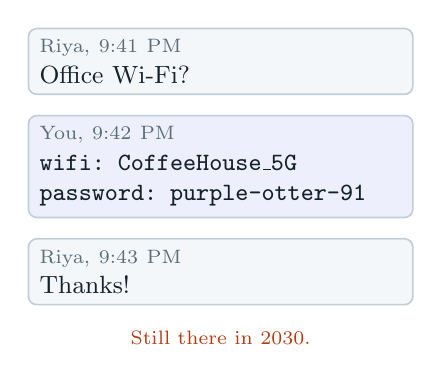
\begin{tikzpicture}[font=\small]
      \node[box, text width=4.6cm, align=left, fill=glass] (c1) {\muted{\scriptsize Riya, 9:41 PM}\\Office Wi-Fi?};
      \node[box, text width=4.6cm, align=left, fill=cobalt!8, below=0.25cm of c1] (c2)
        {\muted{\scriptsize You, 9:42 PM}\\\ttfamily wifi: CoffeeHouse\_5G\\password: purple-otter-91};
      \node[box, text width=4.6cm, align=left, fill=glass, below=0.25cm of c2] (c3) {\muted{\scriptsize Riya, 9:43 PM}\\Thanks!};
      \node[lbl, below=0.2cm of c3, text=ember] {Still there in 2030.};
    \end{tikzpicture}
  \end{columns}
\end{frame}
\note{[A] Think about the last time you sent someone a password. It's probably still sitting in that chat, in cloud backups, maybe in a screenshot. Messages last forever, but secrets shouldn't. And the websites that offer one-time links usually receive your secret in plain text, so you have to trust them completely.}

% ===================================================================================== 4
\begin{frame}{Objectives}
  \begin{enumerate}
    \item \hl{Self-destruct}: a note expires after \emph{N} views or \emph{T} time, whichever comes first.
    \item \hl{Zero knowledge}: the server stores only ciphertext and can never read a note.
    \item \hl{Correct under load}: two people can never both get the last view.
    \item \hl{Containerised}: the whole app runs from Docker images with one command.
    \item \hl{Deployed on a public cloud}: one Amazon EC2 instance, served over HTTPS.
  \end{enumerate}
\end{frame}
\note{[A] We set five objectives. Notes must self-destruct after a number of views or a time limit. The server must never be able to read them. The view limit must hold even when two people open the link at the same moment. The app must be fully containerised. And it must run on a public cloud, Amazon EC2, over HTTPS.}

% ===================================================================================== 5
\section{What Vanish does}
\begin{frame}{How it works for a user}
  \centering
  
\begin{tikzpicture}[node distance=0.55cm]
    \node[flowstep] (s1) {\textbf{Write}\\\scriptsize paste the secret, pick views and expiry};
    \node[flowstep, hot, right=of s1] (s2) {\textbf{Encrypt}\\\scriptsize AES-256-GCM, in the browser};
    \node[flowstep, right=of s2] (s3) {\textbf{Share}\\\scriptsize link with the key after \#, plus QR code};
    \node[flowstep, right=of s3] (s4) {\textbf{Open}\\\scriptsize one view used, decrypted on the device};
    \node[flowstep, right=of s4, draw=ember, text=ember] (s5) {\textbf{Gone}\\\scriptsize deleted at the last view or expiry};
    \foreach \a/\b in {s1/s2, s2/s3, s3/s4, s4/s5} \draw[arr] (\a) -- (\b);
  \end{tikzpicture}
  \vspace{1em}

  \begin{columns}[T]
    \column{0.3\textwidth}\centering \hl{1 to 10} views\\\muted{\small chosen by the sender}
    \column{0.3\textwidth}\centering \hl{5 min to 7 days}\\\muted{\small whichever limit comes first}
    \column{0.3\textwidth}\centering \hl{Optional passphrase}\\\muted{\small a second layer of encryption}
  \end{columns}
\end{frame}
\note{[B] Here's the flow. You write a secret and choose a view limit and an expiry. Your browser encrypts it with AES-256 before anything is sent. You get a link and a QR code. When the recipient opens it, one view is used and the note is decrypted on their device. At the last view, or when time runs out, it's gone for good. You can also add a passphrase as a second lock.}

% ===================================================================================== 6
\begin{frame}{Demo: creating a secret}
  \begin{columns}[T]
    \column{0.49\textwidth}\centering
    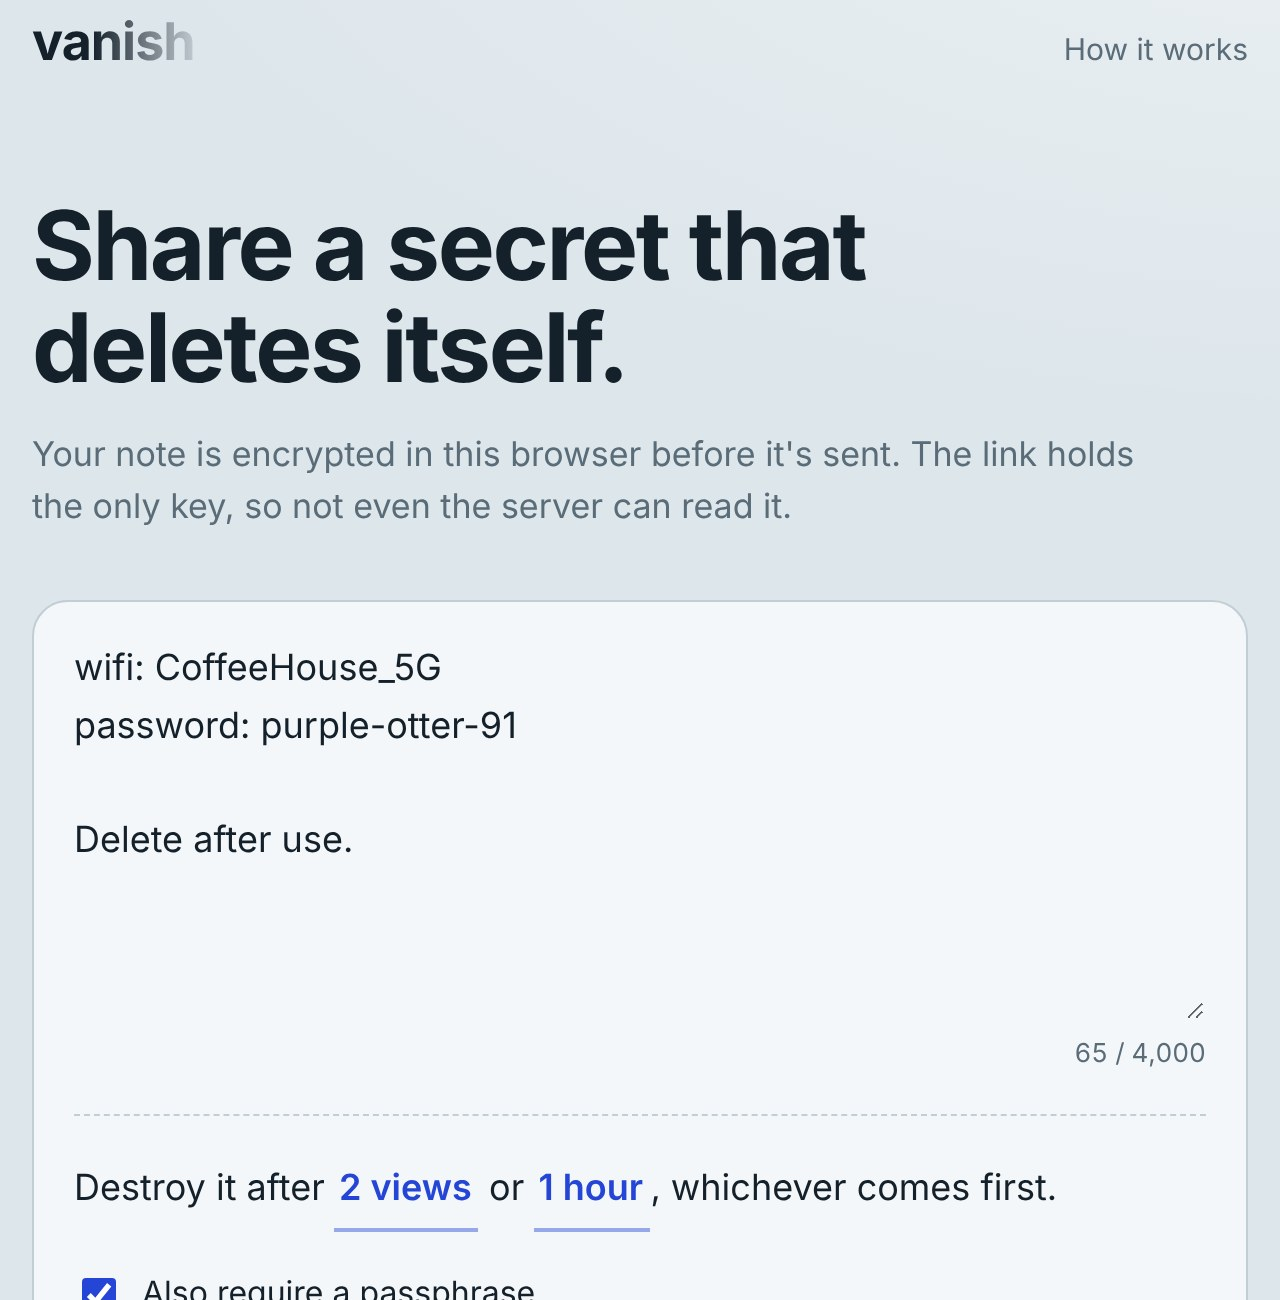
\includegraphics[width=0.84\linewidth]{img/create.jpg}\\[2pt]
    \muted{\scriptsize Write the note; 2 views or 1 hour; passphrase on}
    \column{0.49\textwidth}\centering
    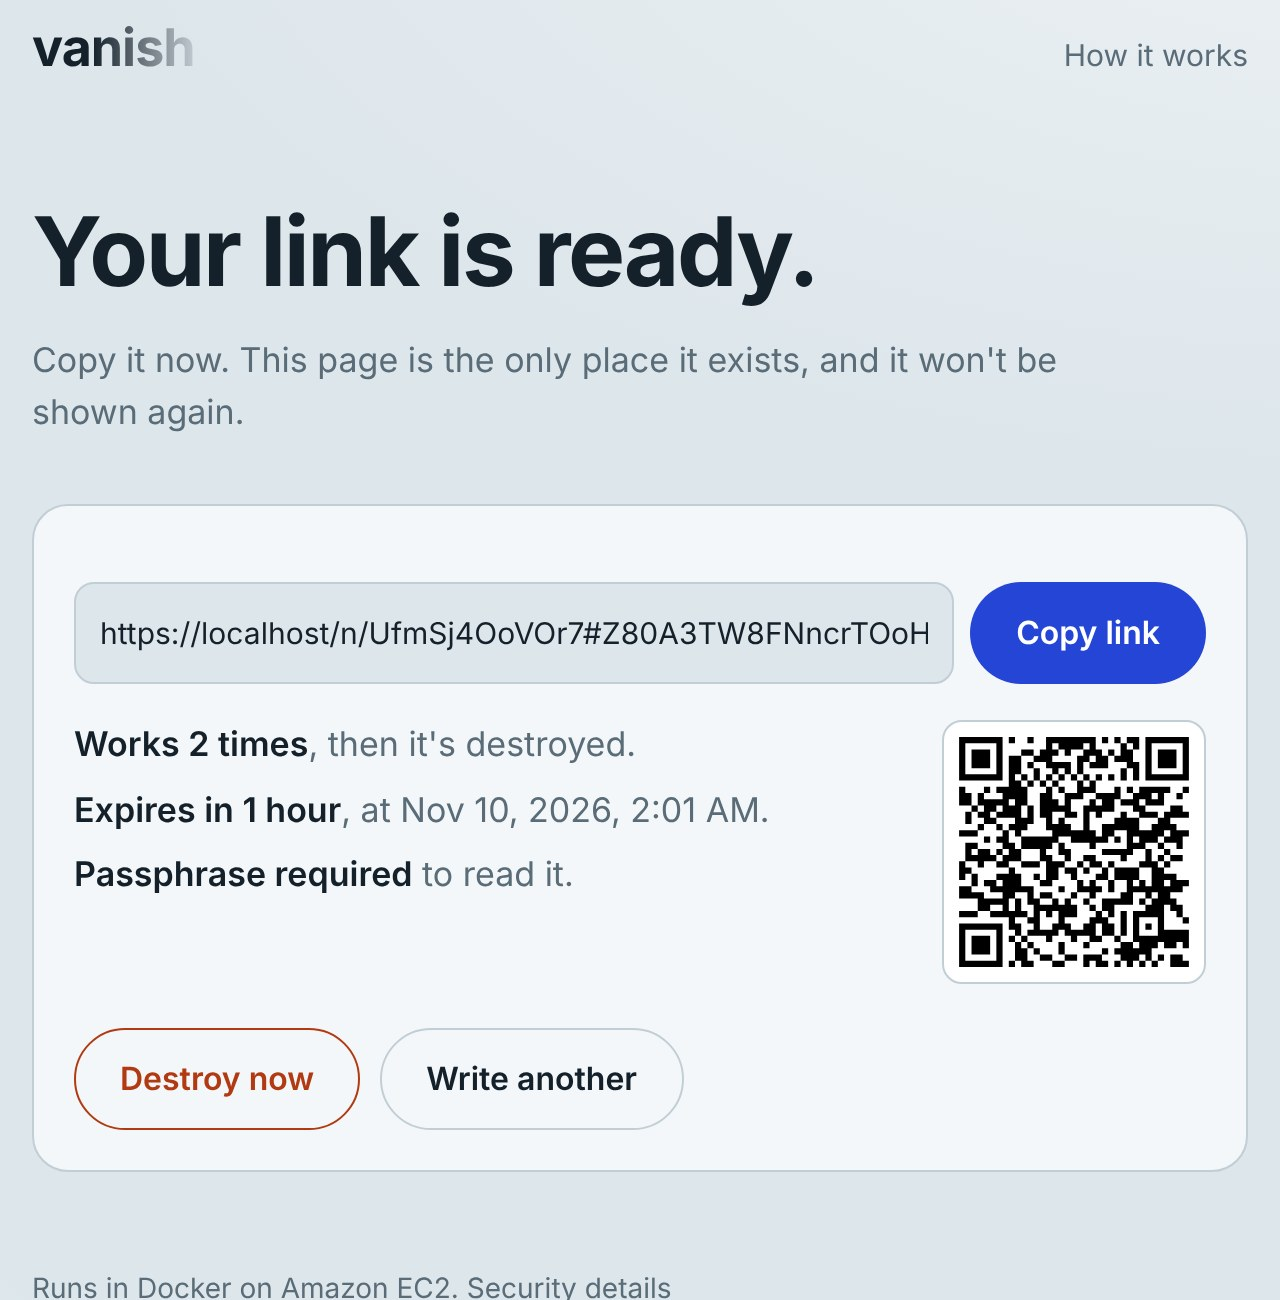
\includegraphics[width=0.84\linewidth]{img/link.jpg}\\[2pt]
    \muted{\scriptsize Encrypted in the browser; link and QR code returned}
  \end{columns}
\end{frame}
\note{[B] This is the app. I paste our café Wi-Fi password, choose two views or one hour, and add the passphrase ``mango''. When I press Create secret link, the text dissolves: it's being encrypted right here in the browser. On the right is the result: the link, a QR code for phones, and a summary of the rules. Only scrambled bytes were sent to the server.}

% ===================================================================================== 7
\begin{frame}{Demo: receiving it, then it vanishes}
  \begin{columns}[T]
    \column{0.32\textwidth}\centering
    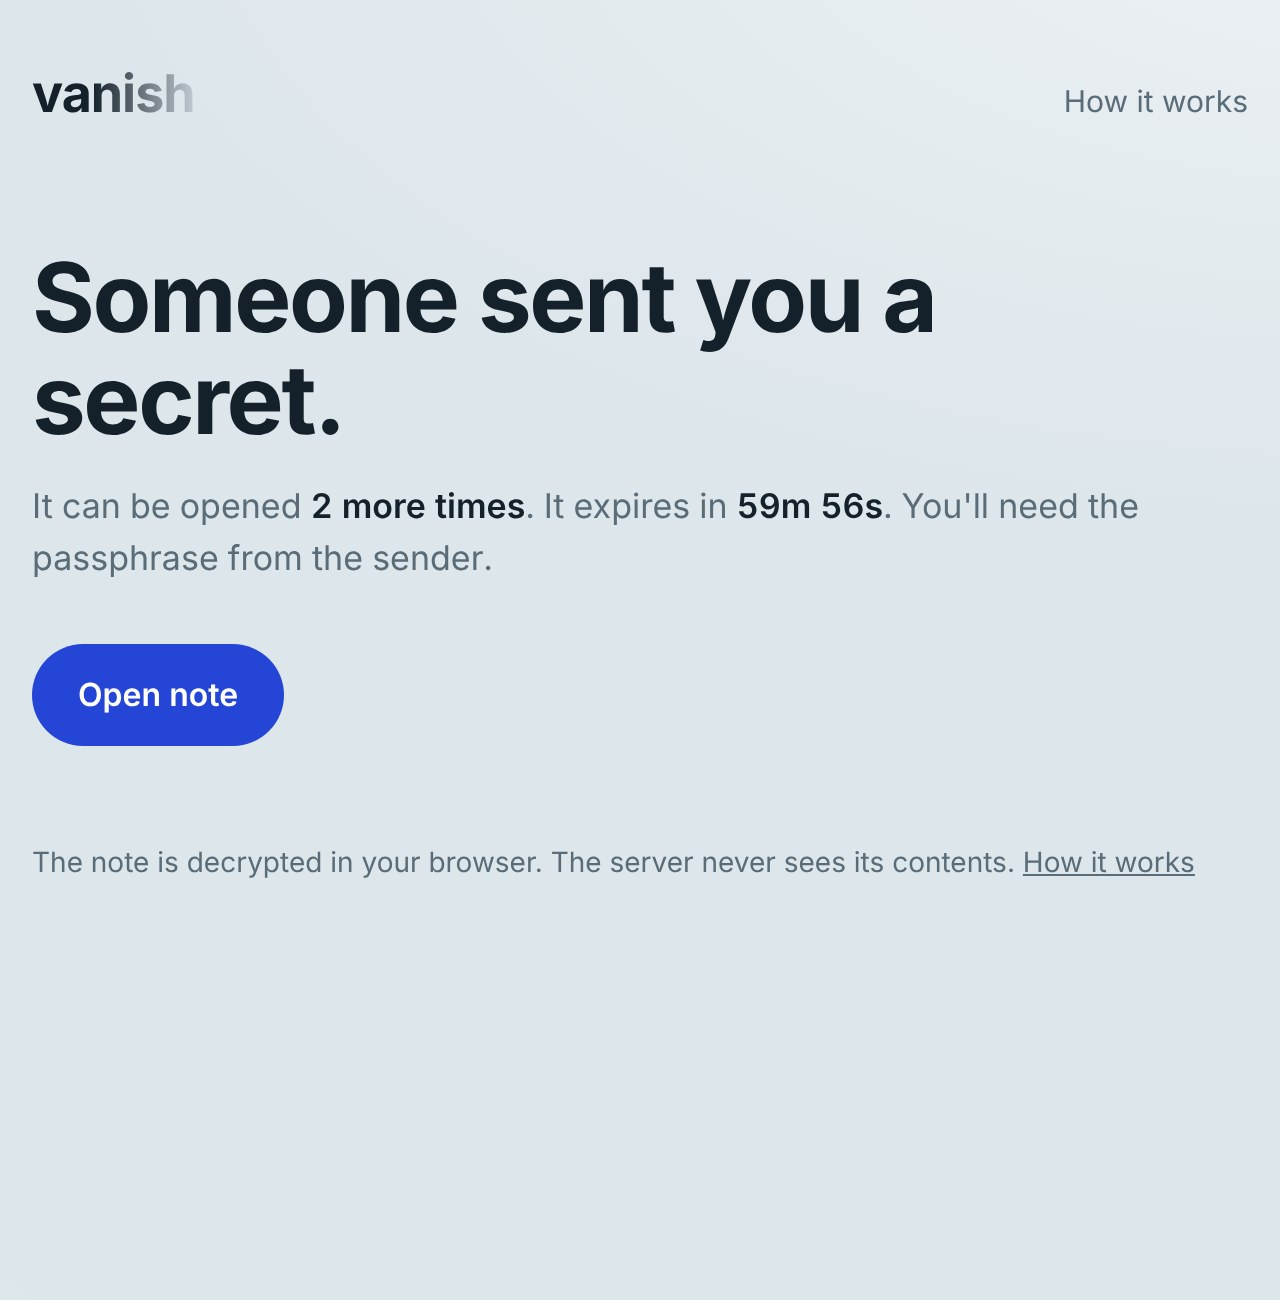
\includegraphics[width=\linewidth]{img/ready.jpg}\\[2pt]
    \muted{\scriptsize Countdown; opening the page uses no view}
    \column{0.32\textwidth}\centering
    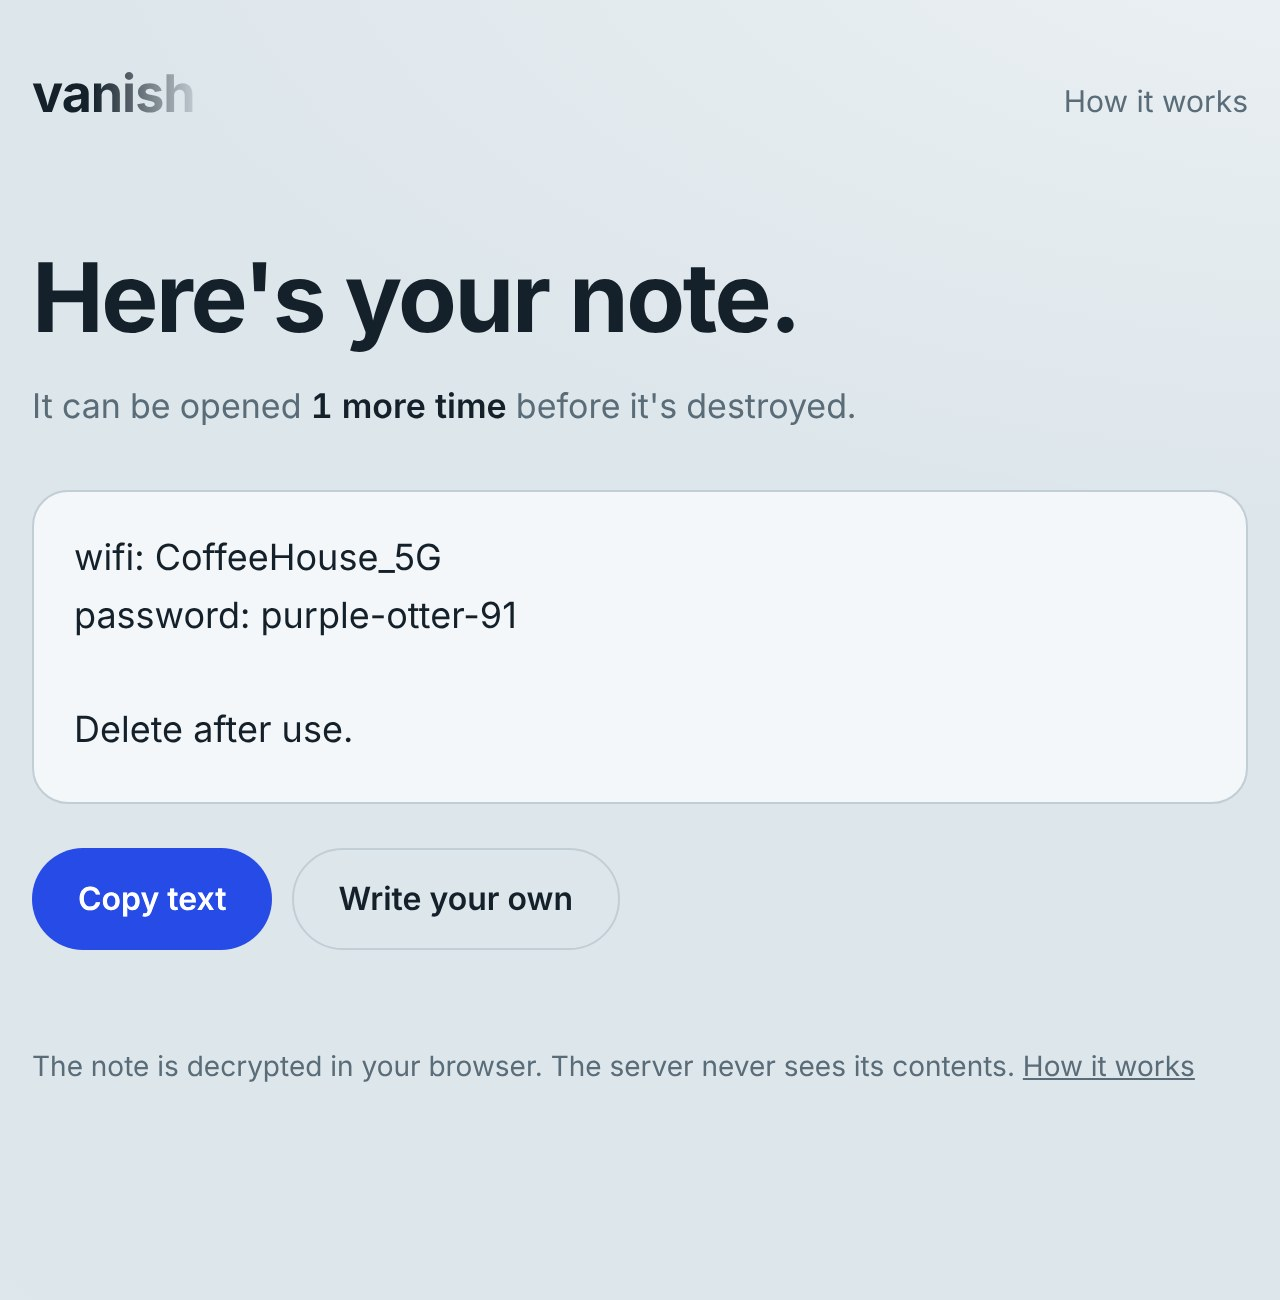
\includegraphics[width=\linewidth]{img/note.jpg}\\[2pt]
    \muted{\scriptsize Decrypted on the recipient's device}
    \column{0.32\textwidth}\centering
    
\includegraphics[width=\linewidth]{img/gone.jpg}\\[2pt]
    \muted{\scriptsize After the last view: nothing left}
  \end{columns}
\end{frame}
\note{[B] The recipient sees that a secret is waiting, how many views remain and a live countdown. Loading this page doesn't use a view, so chat apps that preview links can't burn it by accident. After entering the passphrase, the note is decrypted on their device. Once the last view is used, the server deletes it, and anyone opening the link again sees ``This note has vanished.''}

% ===================================================================================== 8
\section{Architecture}
\begin{frame}{Architecture on Amazon EC2}
  \centering
  \resizebox{\textwidth}{!}{%
  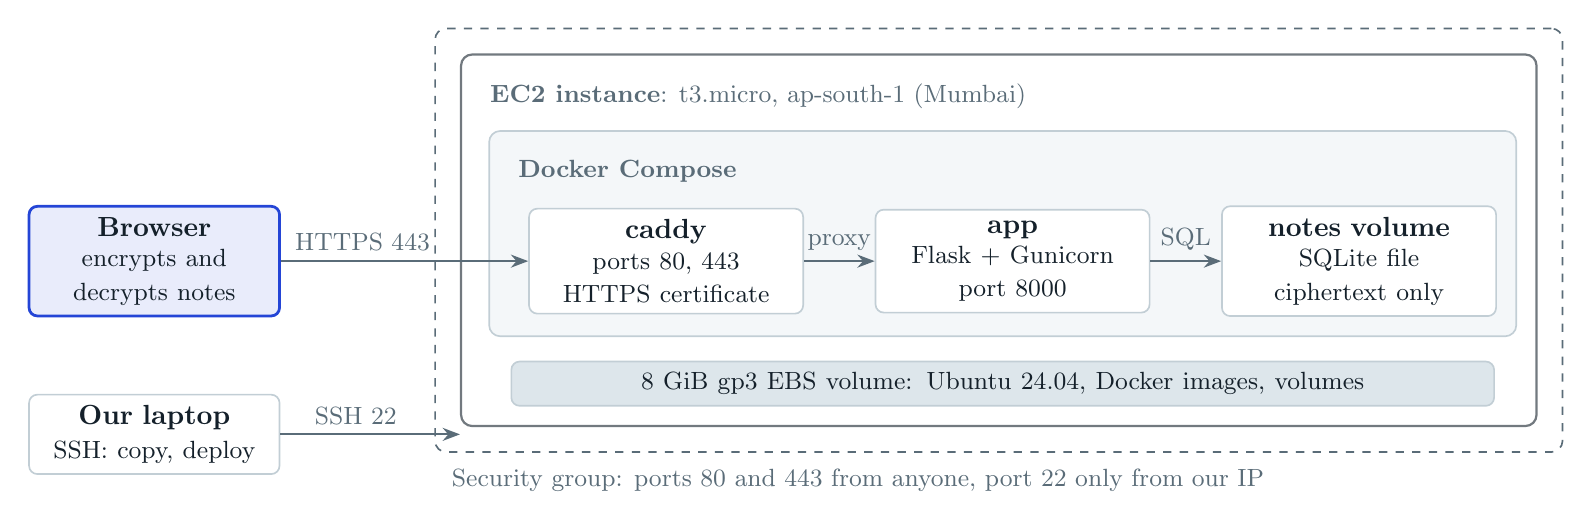
\begin{tikzpicture}[font=\normalsize, box/.append style={font=\normalsize}, hot/.append style={font=\normalsize}, lbl/.append style={font=\small}]
    \node[box, text width=3.2cm] (caddy) at (5.9,2.2) {\textbf{caddy}\\\small ports 80, 443\\HTTPS certificate};
    \node[box, text width=3.2cm] (app) at (10.3,2.2) {\textbf{app}\\\small Flask + Gunicorn\\port 8000};
    \node[box, text width=3.2cm] (vol) at (14.7,2.2) {\textbf{notes volume}\\\small SQLite file\\ciphertext only};
    \node[lbl, anchor=south west] (dcl) at ($(caddy.north west)+(-0.25,0.2)$) {\textbf{Docker Compose}};
    \begin{scope}[on background layer]
      \node[group, fill=glass, fit=(caddy)(app)(vol)(dcl)] (compose) {};
    \end{scope}
    \node[box, fill=fog, text width=12.2cm, anchor=north] (ebs) at ($(compose.south)+(0,-0.3)$)
      {\small 8 GiB gp3 EBS volume: Ubuntu 24.04, Docker images, volumes};
    \node[lbl, anchor=south west] (ecl) at ($(compose.north west)+(-0.1,0.15)$) {\textbf{EC2 instance}: t3.micro, ap-south-1 (Mumbai)};
    \begin{scope}[on background layer]
      \node[group, line width=0.8pt, draw=ink!60, fit=(compose)(ebs)(ecl)] (ec2) {};
      \node[group, dashed, draw=mist, inner sep=9pt, fit=(ec2)] (sg) {};
    \end{scope}
    \node[lbl, anchor=north west] at ($(sg.south west)+(0.1,-0.08)$) {Security group: ports 80 and 443 from anyone, port 22 only from our IP};
    \node[hot, text width=2.9cm] (browser) at (-0.6,2.2) {\textbf{Browser}\\\small encrypts and\\decrypts notes};
    \node[box, text width=2.9cm] (laptop) at (-0.6,0.0) {\textbf{Our laptop}\\\small SSH: copy, deploy};
    \draw[arr] (browser) -- node[lbl, above, pos=0.33] {HTTPS 443} (caddy);
    \draw[arr] (caddy) -- node[lbl, above] {proxy} (app);
    \draw[arr] (app) -- node[lbl, above] {SQL} (vol);
    \draw[arr] (laptop) -- node[lbl, above, pos=0.42] {SSH 22} (laptop -| ec2.west);
  \end{tikzpicture}}
\end{frame}
\note{[C] Everything runs on one Amazon EC2 virtual machine: a t3.micro running Ubuntu in the Mumbai region. A security group, AWS's firewall, lets anyone in on ports 80 and 443, but SSH only from our own IP. Inside, Docker Compose runs two containers. Caddy is the public web server: it gets a free HTTPS certificate and forwards requests to our app container, Flask with Gunicorn. The app keeps notes in a SQLite file on a Docker volume, which lives on the instance's EBS disk.}

% ===================================================================================== 9
\begin{frame}{Cloud services and features used}
  \small
  \begin{tabularx}{\textwidth}{@{}l X l@{}}
    \toprule
    \textbf{Service / feature} & \textbf{How Vanish uses it} & \textbf{Setting} \\
    \midrule
    EC2 instance        & Runs Docker and both containers                    & t3.micro, 2 vCPU, 1 GiB \\
    AMI                 & Operating system image                              & Ubuntu Server 24.04 LTS \\
    User data           & Installs Docker and swap on first boot              & \code{deploy/user-data.sh} \\
    Instance metadata   & \code{deploy.sh} looks up the public IP (IMDSv2)     & 169.254.169.254 \\
    Security group      & Stateful firewall in front of the instance          & 22 (our IP), 80, 443 \\
    Key pair            & Password-less SSH login                              & RSA, \code{.pem} \\
    EBS volume          & Disk for OS, images and the notes database          & 8 GiB gp3 \\
    Public IPv4         & Address users connect to; HTTPS certificate is for it & auto-assigned \\
    EC2 monitoring      & CPU, network and status checks                      & Monitoring tab \\
    \bottomrule
  \end{tabularx}
\end{frame}
\note{[C] These are the EC2 features we used. The instance type and the Ubuntu AMI. A user-data script that installs Docker automatically at first boot. The instance metadata service, which our deploy script queries for the public IP. A security group as the firewall, a key pair for SSH, an 8 GiB EBS volume for storage, the public IPv4 address, and EC2's built-in monitoring.}

% ===================================================================================== 10
\section{Implementation}
\begin{frame}{Zero-knowledge encryption: the key never reaches the server}
  \centering
  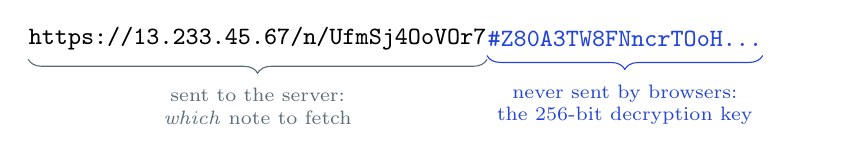
\begin{tikzpicture}
    \node[font=\ttfamily\small, inner sep=0] (a) {https://13.233.45.67/n/UfmSj4OoVOr7};
    \node[font=\ttfamily\small, inner sep=0, anchor=west, text=cobalt] (b) at (a.east) {\#Z80A3TW8FNncrTOoH\dots};
    \draw[decorate, decoration={brace, mirror, amplitude=5pt}, draw=mist] ([yshift=-3pt]a.south west) -- ([yshift=-3pt]a.south east)
      node[midway, below=7pt, lbl, text width=5.2cm, align=center] {sent to the server:\\\textit{which} note to fetch};
    \draw[decorate, decoration={brace, mirror, amplitude=5pt}, draw=cobalt] ([yshift=-3pt]b.south west) -- ([yshift=-3pt]b.south east)
      node[midway, below=7pt, font=\scriptsize, text=cobalt, text width=4.6cm, align=center] {never sent by browsers:\\the 256-bit decryption key};
  \end{tikzpicture}
  \vspace{0.8em}

  \begin{columns}[T]
    \column{0.48\textwidth}
    \begin{itemize}\small
      \item Browser generates a random 256-bit key and encrypts with \hl{AES-256-GCM} (Web Crypto API).
      \item Only \code{\{ciphertext, iv\}} is uploaded.
    \end{itemize}
    \column{0.48\textwidth}
    \begin{itemize}\small
      \item Optional passphrase: second layer, key from \hl{PBKDF2-SHA256}, 310,000 rounds.
      \item GCM is authenticated: tampered data fails to decrypt.
    \end{itemize}
  \end{columns}
\end{frame}
\note{[B] This is the core idea. The part of the link before the hash tells the server which note to fetch. The part after the hash is the 256-bit decryption key, and browsers never send that part to any server. So our EC2 instance only ever stores scrambled ciphertext. Encryption uses AES-256-GCM from the browser's built-in Web Crypto API, and the optional passphrase adds a second layer derived with PBKDF2.}

% ===================================================================================== 11
\begin{frame}{The API: five small endpoints}
  \small
  \begin{tabularx}{\textwidth}{@{}l l X@{}}
    \toprule
    \textbf{Method} & \textbf{Path} & \textbf{What it does} \\
    \midrule
    \code{POST}   & \code{/api/notes}             & Store \code{ciphertext}, \code{iv}, view limit (1--10), expiry (5 min--7 days) \\
    \code{GET}    & \code{/api/notes/\{id\}}      & Views left and expiry; \hl{does not use a view} (safe for link previews) \\
    \code{POST}   & \code{/api/notes/\{id\}/open} & Atomically use one view and return the ciphertext; \code{410 Gone} afterwards \\
    \code{DELETE} & \code{/api/notes/\{id\}}      & Destroy early with the secret delete token (stored as a SHA-256 hash) \\
    \code{GET}    & \code{/api/health}            & Liveness check used by the Docker health check \\
    \bottomrule
  \end{tabularx}
  \vspace{0.8em}

  \muted{A background thread deletes expired notes every 60 seconds; every read also checks the expiry time.}
\end{frame}
\note{[A] The backend is one Python file with five endpoints. Creating a note stores only ciphertext. Reading the metadata never uses a view, which is why WhatsApp previews can't burn a note. Opening uses one view atomically. There's an early-destroy endpoint protected by a secret token, and a health check that Docker uses. A background thread deletes expired notes every minute.}

% ===================================================================================== 12
\begin{frame}[fragile]{Atomic view counting: exactly one winner}
  \begin{columns}[T]
    \column{0.56\textwidth}
\begin{lstlisting}[language=SQL]
UPDATE notes
   SET view_count = view_count + 1
 WHERE id = ?
   AND view_count < max_views
   AND expires_at > ?
RETURNING ciphertext, iv, max_views,
          view_count, expires_at;
\end{lstlisting}
    \small\muted{From \code{open\_note} in \code{app/main.py}. If no row comes back, the API answers \code{410 Gone}.}
    \column{0.40\textwidth}
    \begin{block}{Why one statement?}
      \small
      Check and update happen together, so two people opening the \emph{last} view at the same moment can't both succeed.
    \end{block}
    \vspace{0.4em}
    \begin{exampleblock}{Tested}
      \small 8 simultaneous requests on a 1-view note: \textbf{1} gets the note, \textbf{7} get \code{410}.
    \end{exampleblock}
  \end{columns}
\end{frame}
\note{[A] The most important line of backend code is this single SQL statement. It increases the view count only if the note still has views left and hasn't expired, and returns the note in the same step. Because the check and the update are one atomic operation, two people can't both get the last view. Our test fires eight requests at the same moment at a one-view note: exactly one wins and seven get 410 Gone.}

% ===================================================================================== 13
\section{Docker and deployment}
\begin{frame}[fragile]{Containerising the app: the Dockerfile}
  \begin{columns}[T]
    \column{0.56\textwidth}
\begin{lstlisting}[language=Docker]
FROM python:3.13-slim
ENV DB_PATH=/data/vanish.db
WORKDIR /app
COPY requirements.txt .
RUN pip install --no-cache-dir \
        -r requirements.txt
COPY app/ .
RUN useradd --system --uid 10001 vanish \
 && mkdir -p /data \
 && chown vanish:vanish /data
USER vanish
EXPOSE 8000
HEALTHCHECK CMD python -c "..."  # GET /api/health
CMD ["gunicorn", "--bind", "0.0.0.0:8000",
     "--workers", "1", "--threads", "8",
     "main:app"]
\end{lstlisting}
    \column{0.40\textwidth}
    \begin{itemize}\small
      \item \hl{Slim base image}: small download, fewer packages to patch.
      \item \hl{Dependencies first}: code changes don't re-run \code{pip}.
      \item \hl{Non-root user}: a compromised app can't take over the container.
      \item \hl{Health check}: Docker flags the container if the API stops answering.
      \item \hl{Gunicorn}: production web server, 8 threads.
    \end{itemize}
  \end{columns}
\end{frame}
\note{[C] This is our Dockerfile. It starts from the official slim Python image, installs Flask and Gunicorn first so that code changes rebuild quickly, copies the app, and runs it as a non-root user. A health check calls our API every 30 seconds, and Gunicorn serves the app with eight threads.}

% ===================================================================================== 14
\begin{frame}[fragile]{Two containers: Docker Compose and Caddy}
  \begin{columns}[T]
    \column{0.55\textwidth}
    \small\textbf{compose.yaml} \muted{(abridged)}
\begin{lstlisting}[language=yaml]
services:
  app:
    image: vanish-app:1.0
    build: .
    volumes: ["notes:/data"]
    ports: ["127.0.0.1:8000:8000"]   # private
  caddy:
    image: caddy:2.11
    ports: ["80:80", "443:443"]       # public
    environment:
      SITE_ADDRESS: ${SITE_ADDRESS}
    volumes:
      - ./Caddyfile:/etc/caddy/Caddyfile:ro
      - caddy_data:/data
\end{lstlisting}
    \column{0.41\textwidth}
    \small\textbf{Caddyfile}
\begin{lstlisting}
{
  default_sni {$SITE_ADDRESS}
}
{$SITE_ADDRESS} {
  tls {
    issuer acme {
      profile shortlived
    }
  }
  encode zstd gzip
  reverse_proxy app:8000
}
\end{lstlisting}
    \small\muted{Free Let's Encrypt certificate for the public IP, renewed automatically.}
  \end{columns}
\end{frame}
\note{[C] Docker Compose runs two containers. The app's port is bound to localhost only, so the internet can reach it only through Caddy. Notes live in a named volume, so they survive restarts and rebuilds. On the right is the entire Caddyfile: it requests a free Let's Encrypt certificate for our IP address and forwards every request to the app. HTTPS isn't optional here: browsers only allow the Web Crypto API on secure pages.}

% ===================================================================================== 15
\begin{frame}{Build once, ship the image to EC2}
  \centering
  \resizebox{\textwidth}{!}{%
  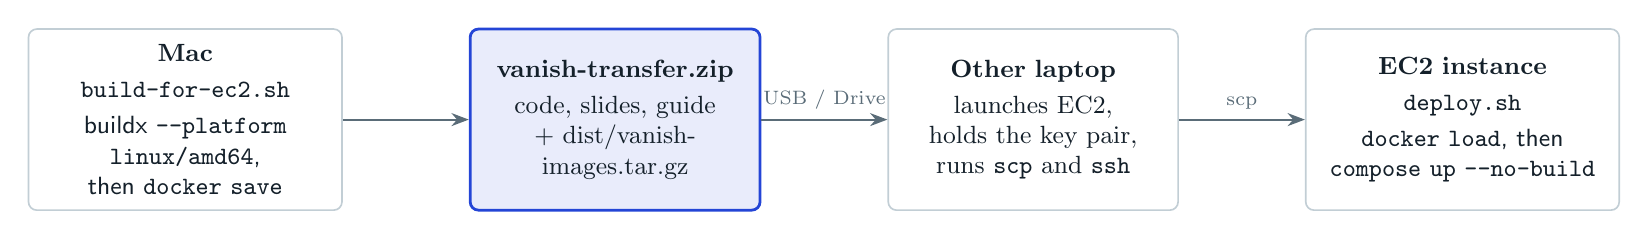
\begin{tikzpicture}[node distance=1.6cm, every node/.append style={font=\normalsize}]
    \node[box, text width=3.7cm, minimum height=2.3cm] (mac) {\textbf{Mac}\\[2pt]\small\ttfamily build-for-ec2.sh\\[2pt]\rmfamily\sffamily buildx \texttt{-{}-platform linux/amd64}, then \texttt{docker save}};
    \node[hot, text width=3.4cm, minimum height=2.3cm, right=of mac] (zip) {\textbf{vanish-transfer.zip}\\[2pt]\small code, slides, guide\\+ dist/vanish-images.tar.gz};
    \node[box, text width=3.4cm, minimum height=2.3cm, right=of zip] (pc) {\textbf{Other laptop}\\[2pt]\small launches EC2, holds the key pair, runs \texttt{scp} and \texttt{ssh}};
    \node[box, text width=3.7cm, minimum height=2.3cm, right=of pc] (ec2) {\textbf{EC2 instance}\\[2pt]\small\ttfamily deploy.sh\\[2pt]\rmfamily\sffamily \texttt{docker load}, then \texttt{compose up -{}-no-build}};
    \draw[arr] (mac) -- (zip);
    \draw[arr] (zip) -- node[lbl, above] {USB / Drive} (pc);
    \draw[arr] (pc) -- node[lbl, above] {scp} (ec2);
  \end{tikzpicture}}
  \vspace{0.9em}

  \begin{alertblock}{Why \texttt{linux/amd64}?}
    \small Apple Silicon Macs build \texttt{arm64} images by default, but a t3.micro has an Intel/AMD processor. A wrong image fails with \emph{exec format error}, so \code{deploy.sh} checks the architecture before starting.
  \end{alertblock}
\end{frame}
\note{[C] We build the images once and ship them. On the Mac, one script builds the app image for linux/amd64, downloads Caddy, and saves both into a single archive inside the project zip. We carry that zip to the laptop we deploy from, copy it to EC2 with scp, and our deploy script loads the images and starts them, with no build on the server. The platform flag matters: Apple Silicon builds arm64 by default, which won't run on a t3.micro, so the deploy script checks this before starting.}

% ===================================================================================== 16
\begin{frame}[fragile]{Deploying on EC2 in four steps}
  \begin{columns}[T]
    \column{0.46\textwidth}
    \begin{enumerate}\small
      \item \textbf{Launch} a t3.micro with Ubuntu 24.04, key pair \code{vanish-key}, HTTP + HTTPS open, SSH from our IP, and \code{user-data.sh} pasted in.
      \item \textbf{Copy} the zip with \code{scp}.
      \item \textbf{Unzip} and run \code{deploy.sh}.
      \item \textbf{Open} \code{https://<public-ip>}.
    \end{enumerate}
    \column{0.52\textwidth}
\begin{lstlisting}[language=bash]
# from the laptop
scp -i vanish-key.pem vanish-transfer.zip \
    ubuntu@13.233.45.67:~
ssh -i vanish-key.pem ubuntu@13.233.45.67

# on the instance
unzip vanish-transfer.zip && cd vanish
bash deploy/deploy.sh
docker compose ps
docker compose logs caddy   # certificate
\end{lstlisting}
  \end{columns}
  \vspace{0.3em}
  \muted{\small \code{deploy.sh} asks the instance metadata service for the public IP, writes it to \code{.env}, loads the images and starts both containers.}
\end{frame}
\note{[C] Deployment takes four steps. We launch a t3.micro with Ubuntu, open HTTP and HTTPS, restrict SSH to our IP, and paste our user-data script, which installs Docker at first boot. Then we copy the zip over with scp, log in with ssh, unzip it and run one script. It finds the public IP from the instance metadata service, loads the images, starts both containers, and Caddy obtains the certificate within a minute.}

% ===================================================================================== 17
\section{Results}
\begin{frame}{Security measures}
  \begin{columns}[T]
    \column{0.48\textwidth}
    \textbf{Data}
    \begin{itemize}\small
      \item Server stores ciphertext, timestamps and counters only
      \item Key in the URL fragment; removed from the address bar after opening
      \item Delete tokens stored as SHA-256 hashes
      \item Notes up to 4,000 characters; 20 new notes per minute per IP
    \end{itemize}
    \column{0.48\textwidth}
    \textbf{Infrastructure}
    \begin{itemize}\small
      \item Security group: only ports 22 (our IP), 80 and 443
      \item App port bound to localhost; only Caddy is public
      \item Container runs as a non-root user
      \item HTTPS everywhere, HSTS, strict Content-Security-Policy, no referrer
    \end{itemize}
  \end{columns}
\end{frame}
\note{[B] Security works in two layers. For data: the server only ever sees ciphertext, the key lives in the URL fragment and is removed from the address bar after opening, delete tokens are hashed, and note creation is rate-limited. For infrastructure: the security group exposes only three ports, the app container isn't directly reachable, it runs as a non-root user, and every response is served over HTTPS with strict browser security headers.}

% ===================================================================================== 18
\begin{frame}{Testing}
  \begin{columns}[T]
    \column{0.40\textwidth}
    \begin{block}{Automated tests (pytest)}
      \centering\vspace{2pt}
      {\Huge\bfseries\color{okgreen} 16 / 16}\\[2pt]
      \small passing
    \end{block}
    \small
    \begin{itemize}
      \item View counting and burn-on-last-view
      \item 8 concurrent opens: exactly 1 winner
      \item Expiry and cleanup, delete tokens
      \item Input validation, rate limit, pages
    \end{itemize}
    \column{0.56\textwidth}
    \textbf{Live checks on the EC2 deployment}
    \small
    \begin{enumerate}
      \item HTTPS loads; \code{http://} redirects to \code{https://}
      \item Create a 2-view note; open it twice; third open shows ``vanished''
      \item Wrong passphrase rejected; right one decrypts
      \item \emph{Destroy now} works; missing key detected
      \item Port 8000 unreachable from the internet
      \item Notes survive \code{docker compose restart}
      \item Database holds ciphertext only
    \end{enumerate}
  \end{columns}
\end{frame}
\note{[A] We tested at two levels. Sixteen automated tests run against the real Flask app and all pass, including the concurrency test. Then on the live EC2 instance we checked HTTPS and the redirect, the full view and burn cycle, the passphrase, early destroy, that port 8000 is closed to the internet, that notes survive a restart, and that the database only contains ciphertext.}

% ===================================================================================== 19
\begin{frame}{Cost}
  \begin{columns}[c]
    \column{0.58\textwidth}
    \small
    \begin{tabularx}{\linewidth}{@{}X r@{}}
      \toprule
      \textbf{Item (ap-south-1, 24/7)} & \textbf{USD / month} \\
      \midrule
      t3.micro instance (\$0.0112 / hour) & $\approx$ 8.20 \\
      Public IPv4 address               & $\approx$ 3.65 \\
      8 GiB gp3 EBS volume              & $\approx$ 0.75 \\
      \midrule
      \textbf{Total}                    & $\approx$ \textbf{12.60} \\
      \bottomrule
    \end{tabularx}
    \column{0.38\textwidth}
    \begin{exampleblock}{Paid by the Free plan}
      \small New AWS accounts get \textbf{\$100 credit}; t3.micro is Free Tier eligible. Our out-of-pocket cost: \textbf{INR 0}.
    \end{exampleblock}
    \vspace{0.3em}
    \muted{\small Stopping the instance when idle leaves only the disk charge.}
  \end{columns}
\end{frame}
\note{[C] Running all month, the instance, its public IP and its disk cost about twelve and a half dollars. New AWS accounts on the Free plan get a hundred dollars of credit and t3.micro is Free Tier eligible, so our out-of-pocket cost was zero. When we aren't using it, we stop the instance, and only the small disk charge remains.}

% ===================================================================================== 20
\section{Conclusion}
\begin{frame}{Challenges and lessons learned}
  \begin{itemize}
    \item \hl{CPU architecture matters.} Images built on an Apple Silicon Mac are \code{arm64}; EC2 t3 is \code{amd64}. Fixed with \code{buildx -{}-platform linux/amd64} and a check in \code{deploy.sh}.
    \item \hl{Browser crypto needs HTTPS.} Web Crypto is disabled on plain \code{http://}, so Caddy with a Let's Encrypt IP certificate is part of the design.
    \item \hl{Public IPs change.} Stopping and starting the instance gives a new IP; re-running \code{deploy.sh} picks it up automatically.
    \item \hl{1 GiB of RAM is tight.} User data adds 1 GiB of swap so builds on the instance never run out of memory.
  \end{itemize}
\end{frame}
\note{[B] We learned a few things the hard way. CPU architecture matters: images from an Apple Silicon Mac won't run on an Intel EC2 instance unless you build for linux/amd64. Browser encryption requires HTTPS, so getting a certificate without a domain became part of the design. Public IPs change when you stop an instance, so the deploy script re-detects it. And a one-gigabyte instance needs swap to build images safely.}

% ===================================================================================== 21
\begin{frame}{Limitations and future work}
  \begin{columns}[T]
    \column{0.47\textwidth}
    \textbf{Limitations}
    \begin{itemize}\small
      \item Anyone holding the full link can read the note; use a passphrase for sensitive data
      \item One instance: no redundancy if it stops
      \item SQLite on one disk: fine for this scale, not for many servers
    \end{itemize}
    \column{0.49\textwidth}
    \textbf{Future work}
    \begin{itemize}\small
      \item Custom domain and an Elastic IP for a stable address
      \item Managed database (Amazon RDS) and two instances behind a load balancer
      \item Image registry (Amazon ECR) and a CI pipeline for builds
      \item File attachments, encrypted the same way
    \end{itemize}
  \end{columns}
\end{frame}
\note{[B] Some honest limits. Anyone with the full link can read the note, so sensitive notes should use a passphrase. One instance means no redundancy, and SQLite suits a single server. Next steps would be a custom domain with a stable Elastic IP, a managed database with two instances behind a load balancer, a container registry with automated builds, and encrypted file attachments.}

% ===================================================================================== 22
\begin{frame}{Summary}
  \begin{columns}[c]
    \column{0.62\textwidth}
    \begin{itemize}
      \item Secrets that \hl{self-destruct} after N views or T time
      \item \hl{Zero-knowledge}: encrypted in the browser, ciphertext on the server
      \item \hl{Atomic} view counting, verified under concurrency
      \item Packaged as \hl{Docker images}, run with Docker Compose
      \item Deployed on \hl{Amazon EC2} over HTTPS, for INR 0
    \end{itemize}
    \column{0.34\textwidth}
    \centering
    {\Large\bfseries Thank you}\\[6pt]
    \muted{Questions?}\\[14pt]
    \small \memberA\\\memberB\\\memberC
  \end{columns}
\end{frame}
\note{[B] To sum up: Vanish lets you share a secret that destroys itself, it never sees your data in plain text, its view limits hold under concurrent access, and the whole thing is packaged with Docker and running on Amazon EC2 over HTTPS, at no cost to us. Thank you for watching.}

\end{document}
"
%  On Overleaf: upload this folder (with img/), set the compiler to pdfLaTeX.
%  For the notes version on Overleaf, uncomment the next line:
% \def\withnotes{}
%
%  Edit the names, college and course in the "EDIT ME" block below.
% =====================================================================================
\documentclass[aspectratio=169,11pt]{beamer}

\usetheme[progressbar=frametitle, numbering=fraction, sectionpage=none, block=fill]{metropolis}

% ---------- fonts: Fira Sans if installed (Overleaf has it), otherwise Helvetica ----------
\usepackage[T1]{fontenc}
\IfFileExists{FiraSans.sty}{%
  \usepackage[sfdefault,scale=0.95]{FiraSans}%
  \usepackage[scale=0.85]{FiraMono}%
}{%
  \usepackage{lmodern}%
  \usepackage[scaled=0.92]{helvet}%
}

\usepackage{tikz}
\usetikzlibrary{positioning, fit, arrows.meta, backgrounds, calc, decorations.pathreplacing, shapes.geometric}
\usepackage{booktabs}
\usepackage{tabularx}
\usepackage{listings}
\usepackage{graphicx}

% ---------- EDIT ME ----------
\newcommand{\memberA}{Member A}
\newcommand{\memberB}{Member B}
\newcommand{\memberC}{Member C}
\newcommand{\college}{Your College Name}
\newcommand{\course}{Cloud Computing Project}
% -----------------------------

% ---------- colours (same palette as the app) ----------
\definecolor{ink}{HTML}{14202A}
\definecolor{mist}{HTML}{5A6C78}
\definecolor{fog}{HTML}{DDE6EB}
\definecolor{glass}{HTML}{F4F7F9}
\definecolor{line}{HTML}{C2CED5}
\definecolor{cobalt}{HTML}{2445D6}
\definecolor{ember}{HTML}{B23A12}
\definecolor{okgreen}{HTML}{1F6F4A}

\setbeamercolor{normal text}{fg=ink, bg=white}
\setbeamercolor{palette primary}{fg=white, bg=ink}
\setbeamercolor{frametitle}{fg=white, bg=ink}
\setbeamercolor{progress bar}{fg=cobalt, bg=fog}
\setbeamercolor{title separator}{fg=cobalt}
\setbeamercolor{alerted text}{fg=ember}
\setbeamercolor{example text}{fg=okgreen}
\setbeamercolor{block title}{fg=ink, bg=fog}
\setbeamercolor{block body}{fg=ink, bg=glass}
\setbeamercolor{itemize item}{fg=cobalt}
\setbeamercolor{enumerate item}{fg=cobalt}
\setbeamercolor{footline}{fg=mist}
\setbeamerfont{frametitle}{size=\large, series=\bfseries}
\setbeamerfont{note page}{size=\normalsize}
\setbeamertemplate{itemize items}{\raisebox{0.15ex}{\scriptsize$\blacktriangleright$}}

\newcommand{\hl}[1]{\textcolor{cobalt}{\textbf{#1}}}
\newcommand{\muted}[1]{\textcolor{mist}{#1}}
\newcommand{\code}[1]{{\ttfamily\small #1}}

% ---------- code listings ----------
\lstdefinelanguage{Docker}{
  morekeywords={FROM,ENV,WORKDIR,COPY,RUN,USER,EXPOSE,HEALTHCHECK,CMD},
  morecomment=[l]{\#}, morestring=[b]"}
\lstdefinelanguage{yaml}{
  morekeywords={services,image,build,restart,volumes,ports,environment,depends_on},
  morecomment=[l]{\#}, morestring=[b]"}
\lstset{
  basicstyle=\ttfamily\scriptsize\color{ink},
  keywordstyle=\color{cobalt}\bfseries,
  commentstyle=\color{mist}\itshape,
  stringstyle=\color{okgreen},
  backgroundcolor=\color{glass},
  frame=single, rulecolor=\color{line}, framesep=4pt, xleftmargin=4pt, xrightmargin=4pt,
  columns=fullflexible, keepspaces=true, showstringspaces=false,
  breaklines=true, aboveskip=2pt, belowskip=2pt, upquote=true
}

% ---------- TikZ styles ----------
\tikzset{
  >={Stealth[length=2.2mm]},
  box/.style={draw=line, line width=0.6pt, rounded corners=3pt, fill=white, align=center,
              inner sep=4pt, font=\small, text=ink},
  hot/.style={box, draw=cobalt, line width=1pt, fill=cobalt!10},
  group/.style={draw=line, line width=0.6pt, rounded corners=4pt, inner sep=7pt},
  arr/.style={->, draw=mist, line width=0.8pt},
  lbl/.style={font=\scriptsize, text=mist},
  flowstep/.style={box, minimum height=1.25cm, text width=2.15cm}
}

% ---------- speaker notes ----------
\ifdefined\withnotes
  \setbeameroption{show only notes}
  \setbeamertemplate{note page}{%
    \vspace{0.3cm}%
    \begin{minipage}[t]{0.36\paperwidth}\insertslideintonotes{0.33}\end{minipage}\hfill
    \begin{minipage}[t]{0.58\paperwidth}\raggedright\normalsize\insertnote\end{minipage}%
  }
\fi

\title{Vanish}
\subtitle{Self-destructing secret notes, containerised with Docker\\and deployed on Amazon EC2}
\author{\memberA \quad\textperiodcentered\quad \memberB \quad\textperiodcentered\quad \memberC}
\institute{\course, \college}
\date{November 2026}
\hypersetup{pdftitle={Vanish: self-destructing secret notes on Amazon EC2}, pdfauthor={\memberA, \memberB, \memberC}}

\begin{document}

% ===================================================================================== 1
\maketitle
\note{[A] Hi, we are \memberA, \memberB\ and \memberC. Our cloud computing project is Vanish: a web app for sharing a secret that deletes itself. We packaged it with Docker and deployed it on an Amazon EC2 virtual machine. In the next ten minutes we'll cover the problem, the design, a demo, how we deployed it, and what we learned.}

% ===================================================================================== 2
\begin{frame}{Agenda}
  \begin{columns}[T]
    \column{0.48\textwidth}
    \begin{enumerate}
      \item The problem and our objectives
      \item What Vanish does: a short demo
      \item Architecture on Amazon EC2
      \item Implementation: encryption, backend
    \end{enumerate}
    \column{0.48\textwidth}
    \begin{enumerate}\setcounter{enumi}{4}
      \item Docker, Docker Compose and Caddy
      \item Building and deploying to EC2
      \item Testing, security and cost
      \item Lessons learned and future work
    \end{enumerate}
  \end{columns}
\end{frame}
\note{[A] Here is our agenda. First the problem and our objectives, then what the app does with real screenshots. \memberC\ will explain the architecture on EC2, \memberA\ and \memberB\ the implementation, and then \memberC\ shows how we containerised and deployed it. We finish with testing, security, cost, and lessons learned.}

% ===================================================================================== 3
\section{Problem and objectives}
\begin{frame}{The problem: secrets live forever in chat history}
  \begin{columns}[c]
    \column{0.52\textwidth}
    \begin{itemize}
      \item We share passwords, Wi-Fi keys and API keys over WhatsApp, email and Slack.
      \item Those messages stay in history, cloud backups and screenshots \hl{indefinitely}.
      \item Existing ``secret sharing'' sites ask you to \alert{trust their server} with the plain text.
    \end{itemize}
    \vspace{0.4em}
    \muted{\small A secret should be readable once, by the right person, and then disappear.}
    \column{0.44\textwidth}
    \centering
    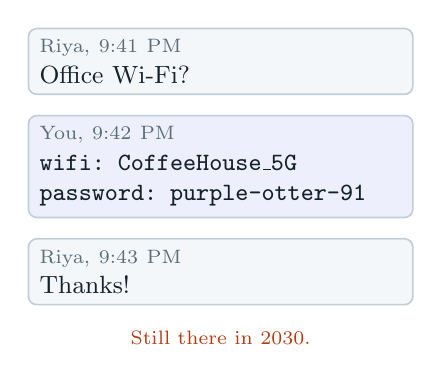
\begin{tikzpicture}[font=\small]
      \node[box, text width=4.6cm, align=left, fill=glass] (c1) {\muted{\scriptsize Riya, 9:41 PM}\\Office Wi-Fi?};
      \node[box, text width=4.6cm, align=left, fill=cobalt!8, below=0.25cm of c1] (c2)
        {\muted{\scriptsize You, 9:42 PM}\\\ttfamily wifi: CoffeeHouse\_5G\\password: purple-otter-91};
      \node[box, text width=4.6cm, align=left, fill=glass, below=0.25cm of c2] (c3) {\muted{\scriptsize Riya, 9:43 PM}\\Thanks!};
      \node[lbl, below=0.2cm of c3, text=ember] {Still there in 2030.};
    \end{tikzpicture}
  \end{columns}
\end{frame}
\note{[A] Think about the last time you sent someone a password. It's probably still sitting in that chat, in cloud backups, maybe in a screenshot. Messages last forever, but secrets shouldn't. And the websites that offer one-time links usually receive your secret in plain text, so you have to trust them completely.}

% ===================================================================================== 4
\begin{frame}{Objectives}
  \begin{enumerate}
    \item \hl{Self-destruct}: a note expires after \emph{N} views or \emph{T} time, whichever comes first.
    \item \hl{Zero knowledge}: the server stores only ciphertext and can never read a note.
    \item \hl{Correct under load}: two people can never both get the last view.
    \item \hl{Containerised}: the whole app runs from Docker images with one command.
    \item \hl{Deployed on a public cloud}: one Amazon EC2 instance, served over HTTPS.
  \end{enumerate}
\end{frame}
\note{[A] We set five objectives. Notes must self-destruct after a number of views or a time limit. The server must never be able to read them. The view limit must hold even when two people open the link at the same moment. The app must be fully containerised. And it must run on a public cloud, Amazon EC2, over HTTPS.}

% ===================================================================================== 5
\section{What Vanish does}
\begin{frame}{How it works for a user}
  \centering
  
\begin{tikzpicture}[node distance=0.55cm]
    \node[flowstep] (s1) {\textbf{Write}\\\scriptsize paste the secret, pick views and expiry};
    \node[flowstep, hot, right=of s1] (s2) {\textbf{Encrypt}\\\scriptsize AES-256-GCM, in the browser};
    \node[flowstep, right=of s2] (s3) {\textbf{Share}\\\scriptsize link with the key after \#, plus QR code};
    \node[flowstep, right=of s3] (s4) {\textbf{Open}\\\scriptsize one view used, decrypted on the device};
    \node[flowstep, right=of s4, draw=ember, text=ember] (s5) {\textbf{Gone}\\\scriptsize deleted at the last view or expiry};
    \foreach \a/\b in {s1/s2, s2/s3, s3/s4, s4/s5} \draw[arr] (\a) -- (\b);
  \end{tikzpicture}
  \vspace{1em}

  \begin{columns}[T]
    \column{0.3\textwidth}\centering \hl{1 to 10} views\\\muted{\small chosen by the sender}
    \column{0.3\textwidth}\centering \hl{5 min to 7 days}\\\muted{\small whichever limit comes first}
    \column{0.3\textwidth}\centering \hl{Optional passphrase}\\\muted{\small a second layer of encryption}
  \end{columns}
\end{frame}
\note{[B] Here's the flow. You write a secret and choose a view limit and an expiry. Your browser encrypts it with AES-256 before anything is sent. You get a link and a QR code. When the recipient opens it, one view is used and the note is decrypted on their device. At the last view, or when time runs out, it's gone for good. You can also add a passphrase as a second lock.}

% ===================================================================================== 6
\begin{frame}{Demo: creating a secret}
  \begin{columns}[T]
    \column{0.49\textwidth}\centering
    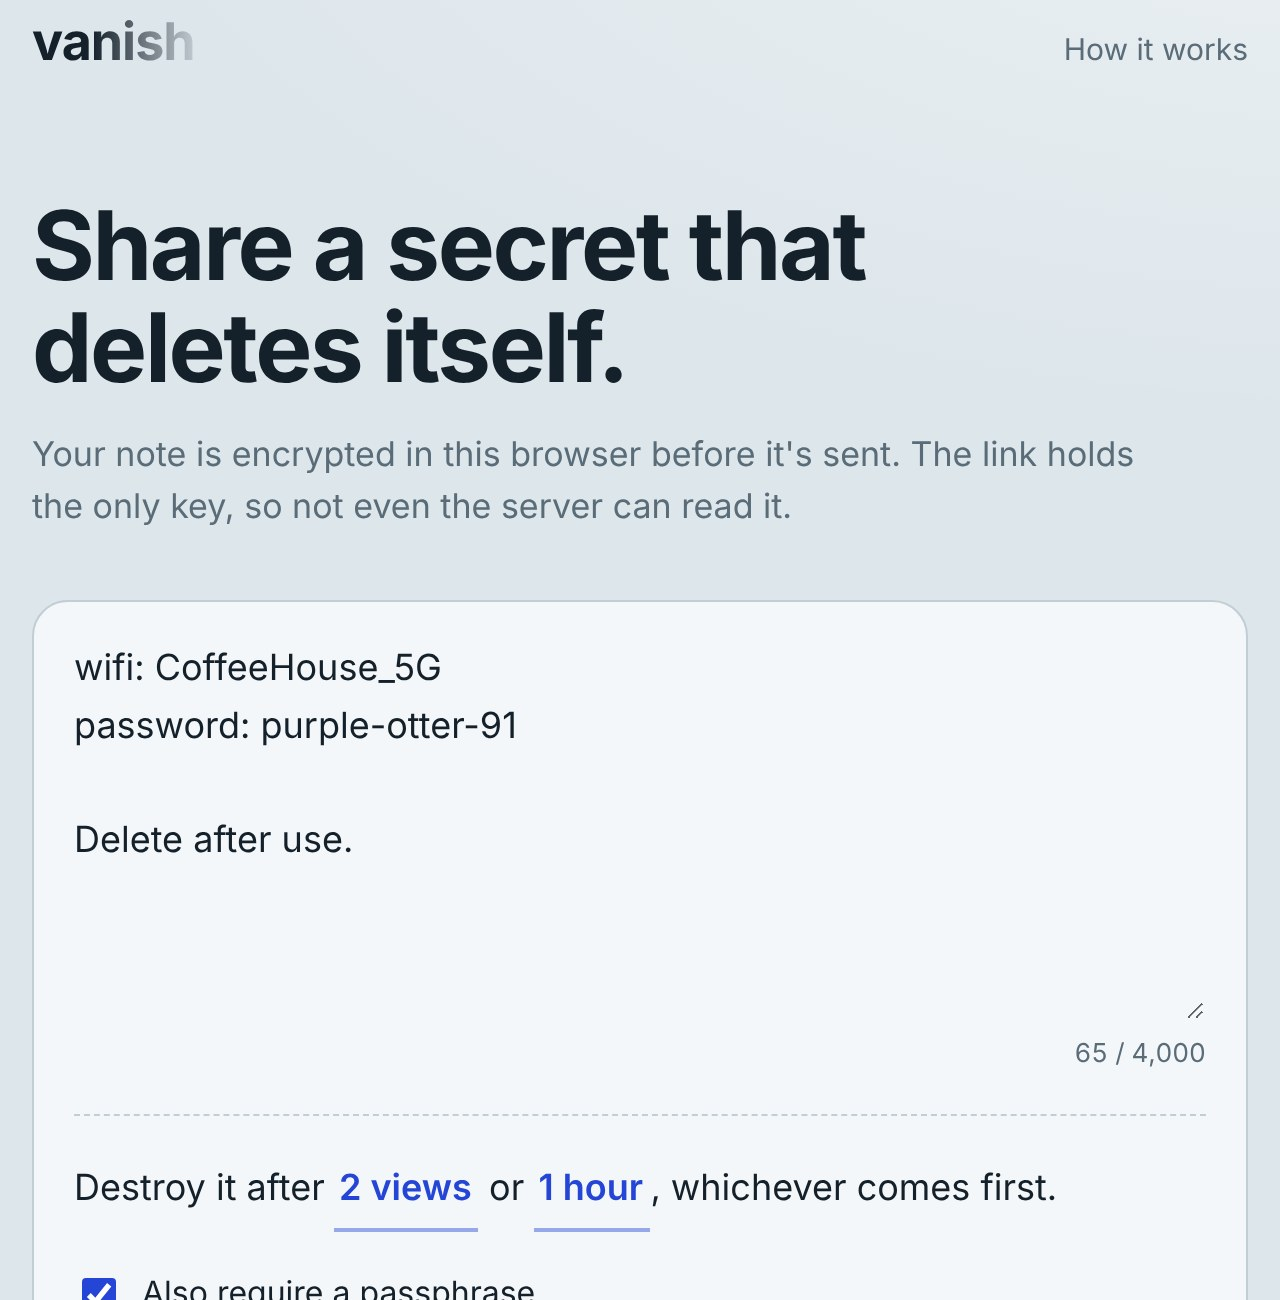
\includegraphics[width=0.84\linewidth]{img/create.jpg}\\[2pt]
    \muted{\scriptsize Write the note; 2 views or 1 hour; passphrase on}
    \column{0.49\textwidth}\centering
    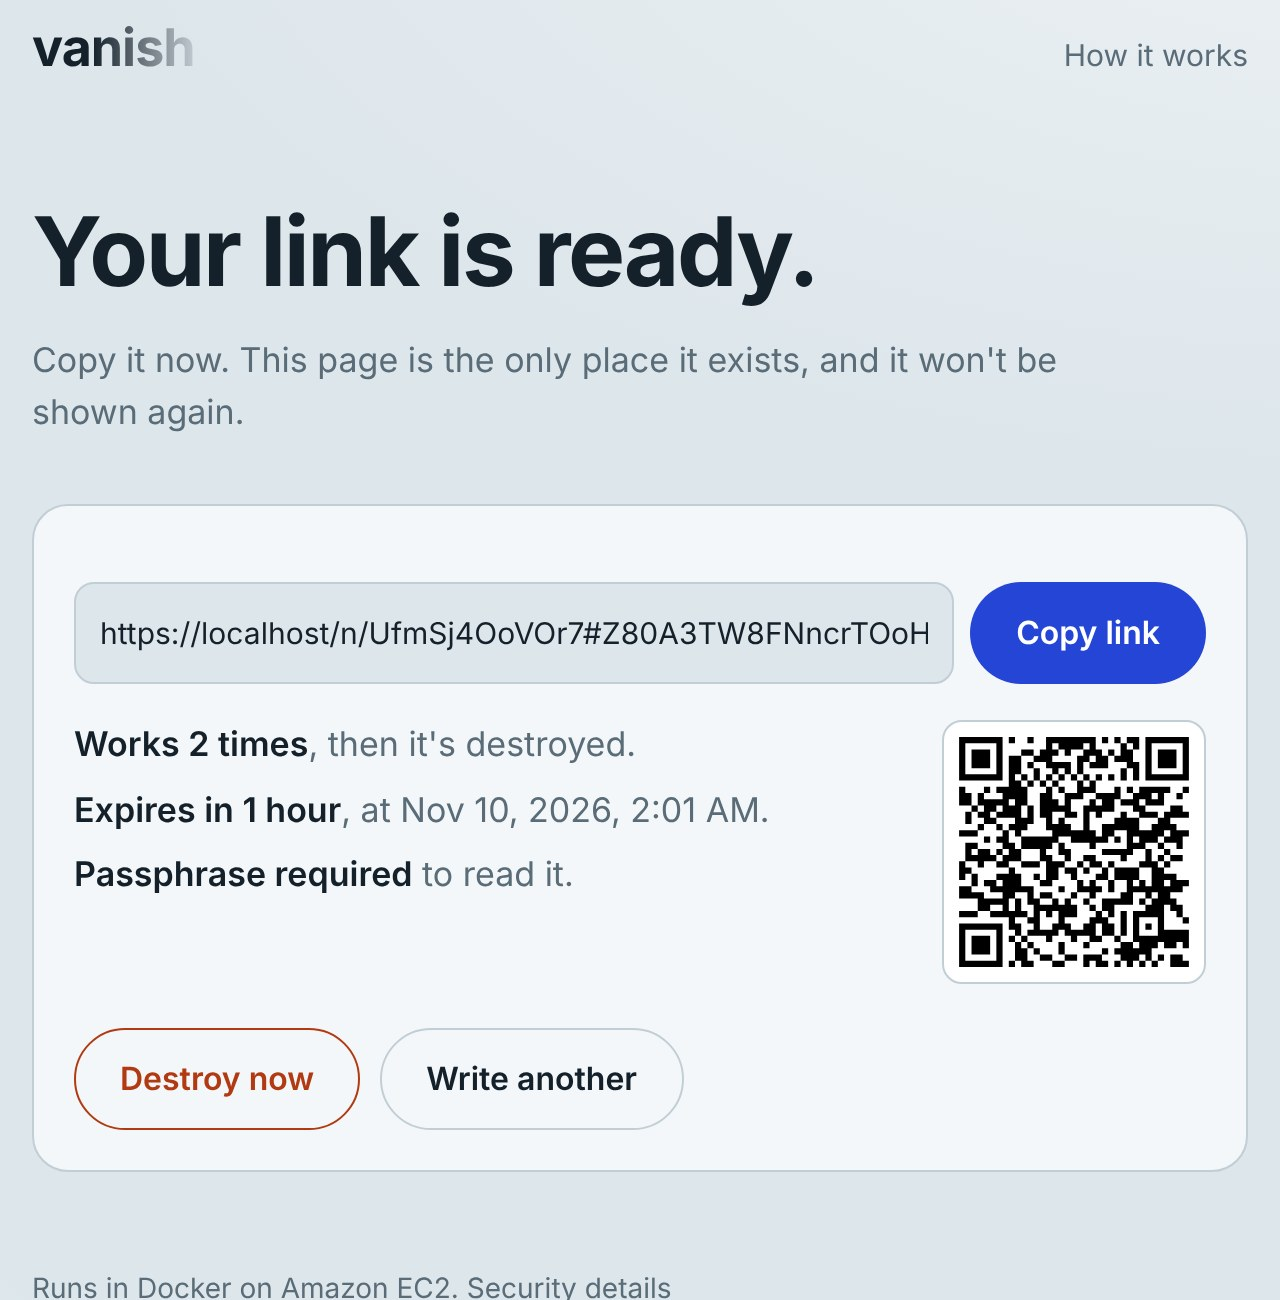
\includegraphics[width=0.84\linewidth]{img/link.jpg}\\[2pt]
    \muted{\scriptsize Encrypted in the browser; link and QR code returned}
  \end{columns}
\end{frame}
\note{[B] This is the app. I paste our café Wi-Fi password, choose two views or one hour, and add the passphrase ``mango''. When I press Create secret link, the text dissolves: it's being encrypted right here in the browser. On the right is the result: the link, a QR code for phones, and a summary of the rules. Only scrambled bytes were sent to the server.}

% ===================================================================================== 7
\begin{frame}{Demo: receiving it, then it vanishes}
  \begin{columns}[T]
    \column{0.32\textwidth}\centering
    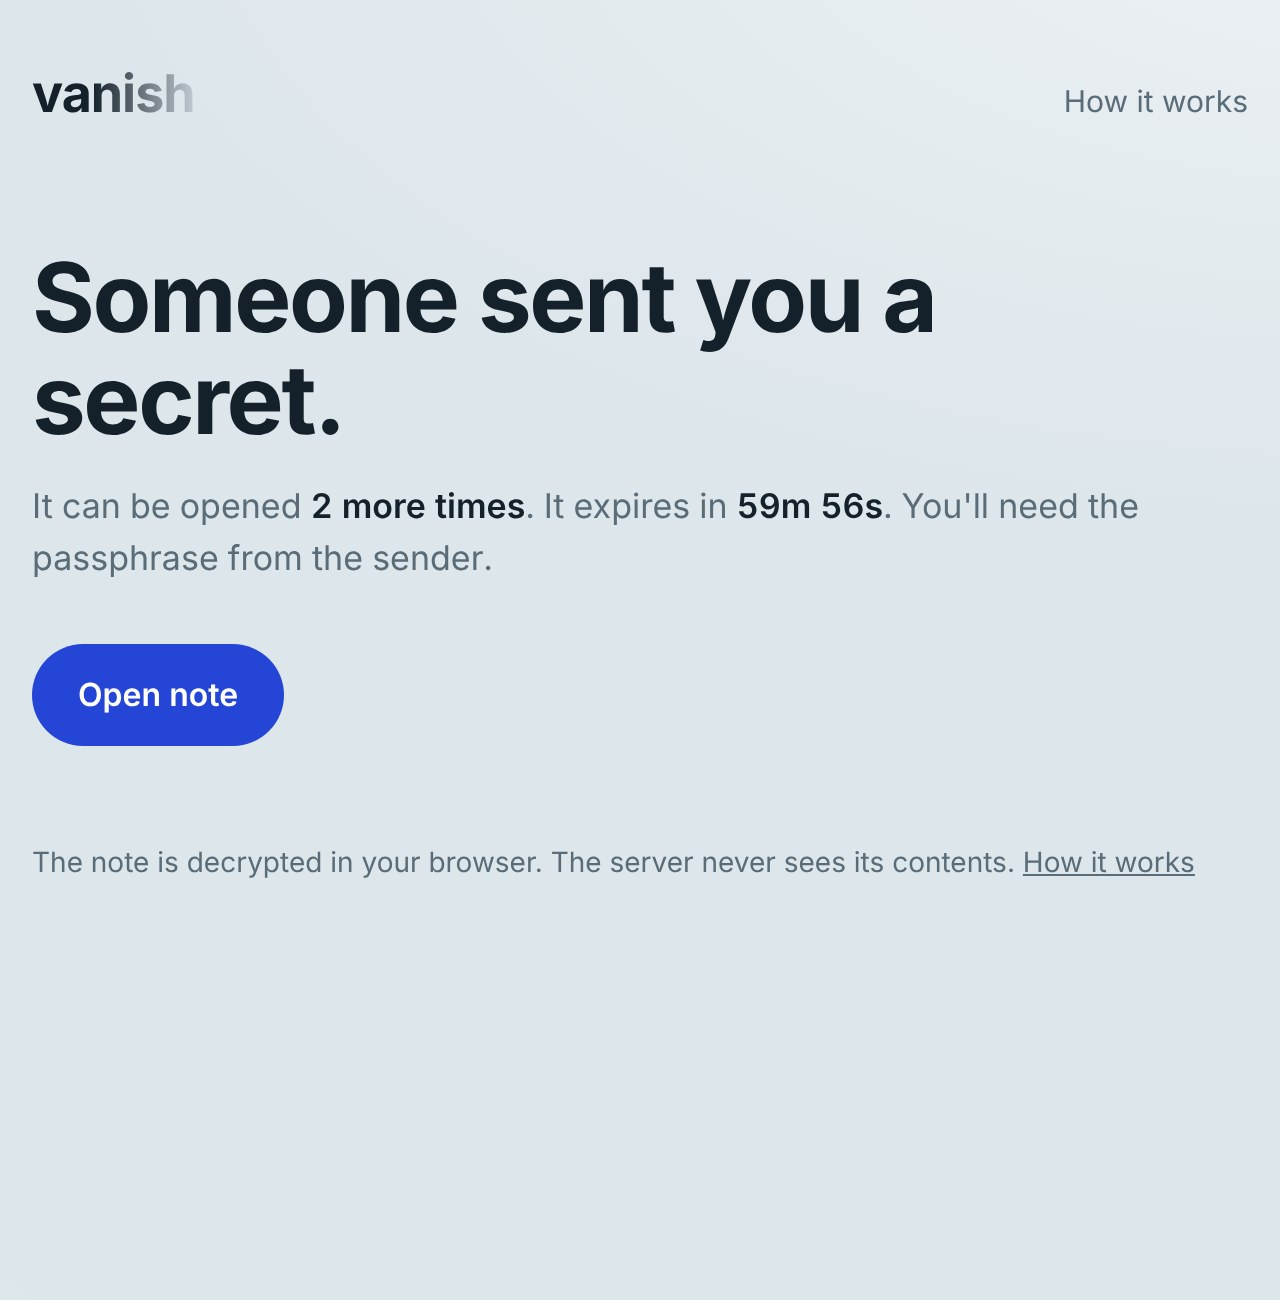
\includegraphics[width=\linewidth]{img/ready.jpg}\\[2pt]
    \muted{\scriptsize Countdown; opening the page uses no view}
    \column{0.32\textwidth}\centering
    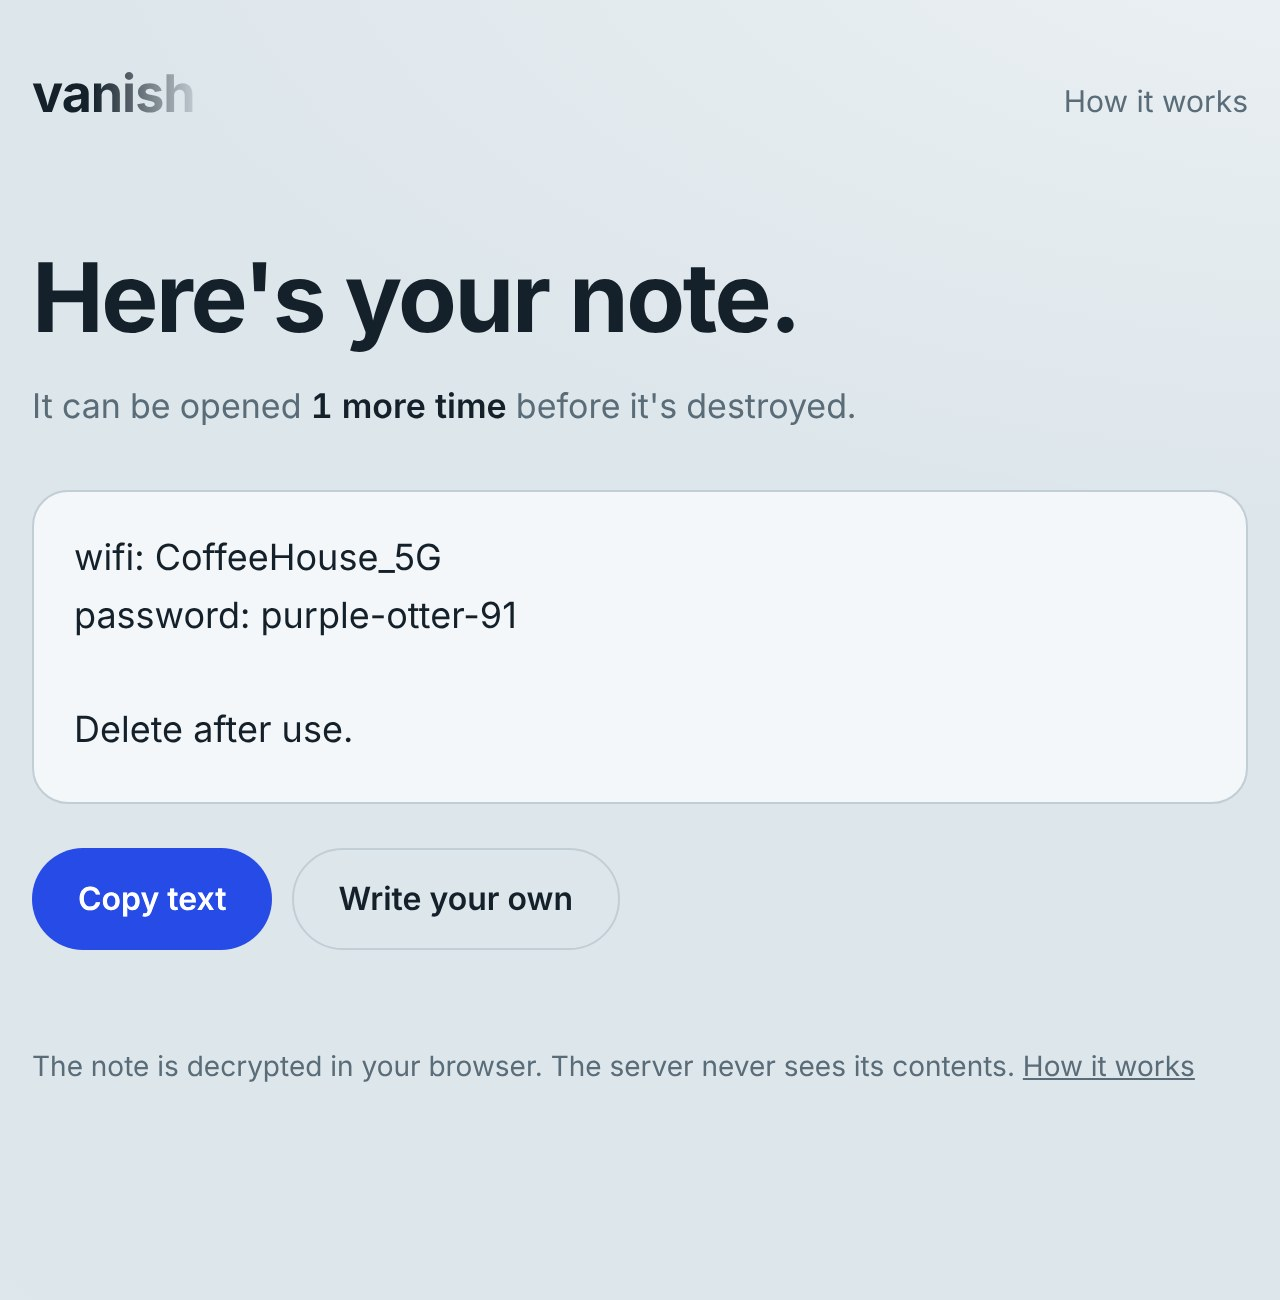
\includegraphics[width=\linewidth]{img/note.jpg}\\[2pt]
    \muted{\scriptsize Decrypted on the recipient's device}
    \column{0.32\textwidth}\centering
    
\includegraphics[width=\linewidth]{img/gone.jpg}\\[2pt]
    \muted{\scriptsize After the last view: nothing left}
  \end{columns}
\end{frame}
\note{[B] The recipient sees that a secret is waiting, how many views remain and a live countdown. Loading this page doesn't use a view, so chat apps that preview links can't burn it by accident. After entering the passphrase, the note is decrypted on their device. Once the last view is used, the server deletes it, and anyone opening the link again sees ``This note has vanished.''}

% ===================================================================================== 8
\section{Architecture}
\begin{frame}{Architecture on Amazon EC2}
  \centering
  \resizebox{\textwidth}{!}{%
  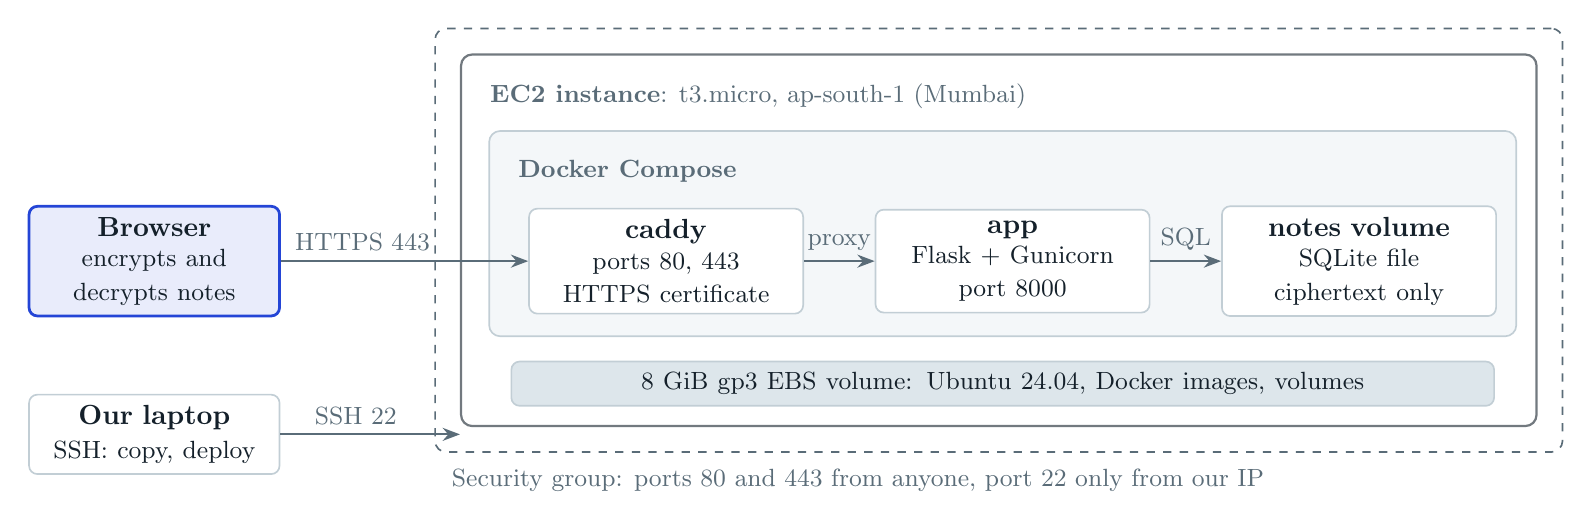
\begin{tikzpicture}[font=\normalsize, box/.append style={font=\normalsize}, hot/.append style={font=\normalsize}, lbl/.append style={font=\small}]
    \node[box, text width=3.2cm] (caddy) at (5.9,2.2) {\textbf{caddy}\\\small ports 80, 443\\HTTPS certificate};
    \node[box, text width=3.2cm] (app) at (10.3,2.2) {\textbf{app}\\\small Flask + Gunicorn\\port 8000};
    \node[box, text width=3.2cm] (vol) at (14.7,2.2) {\textbf{notes volume}\\\small SQLite file\\ciphertext only};
    \node[lbl, anchor=south west] (dcl) at ($(caddy.north west)+(-0.25,0.2)$) {\textbf{Docker Compose}};
    \begin{scope}[on background layer]
      \node[group, fill=glass, fit=(caddy)(app)(vol)(dcl)] (compose) {};
    \end{scope}
    \node[box, fill=fog, text width=12.2cm, anchor=north] (ebs) at ($(compose.south)+(0,-0.3)$)
      {\small 8 GiB gp3 EBS volume: Ubuntu 24.04, Docker images, volumes};
    \node[lbl, anchor=south west] (ecl) at ($(compose.north west)+(-0.1,0.15)$) {\textbf{EC2 instance}: t3.micro, ap-south-1 (Mumbai)};
    \begin{scope}[on background layer]
      \node[group, line width=0.8pt, draw=ink!60, fit=(compose)(ebs)(ecl)] (ec2) {};
      \node[group, dashed, draw=mist, inner sep=9pt, fit=(ec2)] (sg) {};
    \end{scope}
    \node[lbl, anchor=north west] at ($(sg.south west)+(0.1,-0.08)$) {Security group: ports 80 and 443 from anyone, port 22 only from our IP};
    \node[hot, text width=2.9cm] (browser) at (-0.6,2.2) {\textbf{Browser}\\\small encrypts and\\decrypts notes};
    \node[box, text width=2.9cm] (laptop) at (-0.6,0.0) {\textbf{Our laptop}\\\small SSH: copy, deploy};
    \draw[arr] (browser) -- node[lbl, above, pos=0.33] {HTTPS 443} (caddy);
    \draw[arr] (caddy) -- node[lbl, above] {proxy} (app);
    \draw[arr] (app) -- node[lbl, above] {SQL} (vol);
    \draw[arr] (laptop) -- node[lbl, above, pos=0.42] {SSH 22} (laptop -| ec2.west);
  \end{tikzpicture}}
\end{frame}
\note{[C] Everything runs on one Amazon EC2 virtual machine: a t3.micro running Ubuntu in the Mumbai region. A security group, AWS's firewall, lets anyone in on ports 80 and 443, but SSH only from our own IP. Inside, Docker Compose runs two containers. Caddy is the public web server: it gets a free HTTPS certificate and forwards requests to our app container, Flask with Gunicorn. The app keeps notes in a SQLite file on a Docker volume, which lives on the instance's EBS disk.}

% ===================================================================================== 9
\begin{frame}{Cloud services and features used}
  \small
  \begin{tabularx}{\textwidth}{@{}l X l@{}}
    \toprule
    \textbf{Service / feature} & \textbf{How Vanish uses it} & \textbf{Setting} \\
    \midrule
    EC2 instance        & Runs Docker and both containers                    & t3.micro, 2 vCPU, 1 GiB \\
    AMI                 & Operating system image                              & Ubuntu Server 24.04 LTS \\
    User data           & Installs Docker and swap on first boot              & \code{deploy/user-data.sh} \\
    Instance metadata   & \code{deploy.sh} looks up the public IP (IMDSv2)     & 169.254.169.254 \\
    Security group      & Stateful firewall in front of the instance          & 22 (our IP), 80, 443 \\
    Key pair            & Password-less SSH login                              & RSA, \code{.pem} \\
    EBS volume          & Disk for OS, images and the notes database          & 8 GiB gp3 \\
    Public IPv4         & Address users connect to; HTTPS certificate is for it & auto-assigned \\
    EC2 monitoring      & CPU, network and status checks                      & Monitoring tab \\
    \bottomrule
  \end{tabularx}
\end{frame}
\note{[C] These are the EC2 features we used. The instance type and the Ubuntu AMI. A user-data script that installs Docker automatically at first boot. The instance metadata service, which our deploy script queries for the public IP. A security group as the firewall, a key pair for SSH, an 8 GiB EBS volume for storage, the public IPv4 address, and EC2's built-in monitoring.}

% ===================================================================================== 10
\section{Implementation}
\begin{frame}{Zero-knowledge encryption: the key never reaches the server}
  \centering
  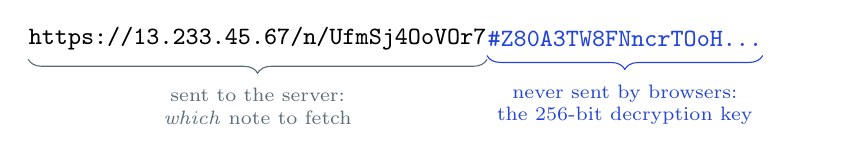
\begin{tikzpicture}
    \node[font=\ttfamily\small, inner sep=0] (a) {https://13.233.45.67/n/UfmSj4OoVOr7};
    \node[font=\ttfamily\small, inner sep=0, anchor=west, text=cobalt] (b) at (a.east) {\#Z80A3TW8FNncrTOoH\dots};
    \draw[decorate, decoration={brace, mirror, amplitude=5pt}, draw=mist] ([yshift=-3pt]a.south west) -- ([yshift=-3pt]a.south east)
      node[midway, below=7pt, lbl, text width=5.2cm, align=center] {sent to the server:\\\textit{which} note to fetch};
    \draw[decorate, decoration={brace, mirror, amplitude=5pt}, draw=cobalt] ([yshift=-3pt]b.south west) -- ([yshift=-3pt]b.south east)
      node[midway, below=7pt, font=\scriptsize, text=cobalt, text width=4.6cm, align=center] {never sent by browsers:\\the 256-bit decryption key};
  \end{tikzpicture}
  \vspace{0.8em}

  \begin{columns}[T]
    \column{0.48\textwidth}
    \begin{itemize}\small
      \item Browser generates a random 256-bit key and encrypts with \hl{AES-256-GCM} (Web Crypto API).
      \item Only \code{\{ciphertext, iv\}} is uploaded.
    \end{itemize}
    \column{0.48\textwidth}
    \begin{itemize}\small
      \item Optional passphrase: second layer, key from \hl{PBKDF2-SHA256}, 310,000 rounds.
      \item GCM is authenticated: tampered data fails to decrypt.
    \end{itemize}
  \end{columns}
\end{frame}
\note{[B] This is the core idea. The part of the link before the hash tells the server which note to fetch. The part after the hash is the 256-bit decryption key, and browsers never send that part to any server. So our EC2 instance only ever stores scrambled ciphertext. Encryption uses AES-256-GCM from the browser's built-in Web Crypto API, and the optional passphrase adds a second layer derived with PBKDF2.}

% ===================================================================================== 11
\begin{frame}{The API: five small endpoints}
  \small
  \begin{tabularx}{\textwidth}{@{}l l X@{}}
    \toprule
    \textbf{Method} & \textbf{Path} & \textbf{What it does} \\
    \midrule
    \code{POST}   & \code{/api/notes}             & Store \code{ciphertext}, \code{iv}, view limit (1--10), expiry (5 min--7 days) \\
    \code{GET}    & \code{/api/notes/\{id\}}      & Views left and expiry; \hl{does not use a view} (safe for link previews) \\
    \code{POST}   & \code{/api/notes/\{id\}/open} & Atomically use one view and return the ciphertext; \code{410 Gone} afterwards \\
    \code{DELETE} & \code{/api/notes/\{id\}}      & Destroy early with the secret delete token (stored as a SHA-256 hash) \\
    \code{GET}    & \code{/api/health}            & Liveness check used by the Docker health check \\
    \bottomrule
  \end{tabularx}
  \vspace{0.8em}

  \muted{A background thread deletes expired notes every 60 seconds; every read also checks the expiry time.}
\end{frame}
\note{[A] The backend is one Python file with five endpoints. Creating a note stores only ciphertext. Reading the metadata never uses a view, which is why WhatsApp previews can't burn a note. Opening uses one view atomically. There's an early-destroy endpoint protected by a secret token, and a health check that Docker uses. A background thread deletes expired notes every minute.}

% ===================================================================================== 12
\begin{frame}[fragile]{Atomic view counting: exactly one winner}
  \begin{columns}[T]
    \column{0.56\textwidth}
\begin{lstlisting}[language=SQL]
UPDATE notes
   SET view_count = view_count + 1
 WHERE id = ?
   AND view_count < max_views
   AND expires_at > ?
RETURNING ciphertext, iv, max_views,
          view_count, expires_at;
\end{lstlisting}
    \small\muted{From \code{open\_note} in \code{app/main.py}. If no row comes back, the API answers \code{410 Gone}.}
    \column{0.40\textwidth}
    \begin{block}{Why one statement?}
      \small
      Check and update happen together, so two people opening the \emph{last} view at the same moment can't both succeed.
    \end{block}
    \vspace{0.4em}
    \begin{exampleblock}{Tested}
      \small 8 simultaneous requests on a 1-view note: \textbf{1} gets the note, \textbf{7} get \code{410}.
    \end{exampleblock}
  \end{columns}
\end{frame}
\note{[A] The most important line of backend code is this single SQL statement. It increases the view count only if the note still has views left and hasn't expired, and returns the note in the same step. Because the check and the update are one atomic operation, two people can't both get the last view. Our test fires eight requests at the same moment at a one-view note: exactly one wins and seven get 410 Gone.}

% ===================================================================================== 13
\section{Docker and deployment}
\begin{frame}[fragile]{Containerising the app: the Dockerfile}
  \begin{columns}[T]
    \column{0.56\textwidth}
\begin{lstlisting}[language=Docker]
FROM python:3.13-slim
ENV DB_PATH=/data/vanish.db
WORKDIR /app
COPY requirements.txt .
RUN pip install --no-cache-dir \
        -r requirements.txt
COPY app/ .
RUN useradd --system --uid 10001 vanish \
 && mkdir -p /data \
 && chown vanish:vanish /data
USER vanish
EXPOSE 8000
HEALTHCHECK CMD python -c "..."  # GET /api/health
CMD ["gunicorn", "--bind", "0.0.0.0:8000",
     "--workers", "1", "--threads", "8",
     "main:app"]
\end{lstlisting}
    \column{0.40\textwidth}
    \begin{itemize}\small
      \item \hl{Slim base image}: small download, fewer packages to patch.
      \item \hl{Dependencies first}: code changes don't re-run \code{pip}.
      \item \hl{Non-root user}: a compromised app can't take over the container.
      \item \hl{Health check}: Docker flags the container if the API stops answering.
      \item \hl{Gunicorn}: production web server, 8 threads.
    \end{itemize}
  \end{columns}
\end{frame}
\note{[C] This is our Dockerfile. It starts from the official slim Python image, installs Flask and Gunicorn first so that code changes rebuild quickly, copies the app, and runs it as a non-root user. A health check calls our API every 30 seconds, and Gunicorn serves the app with eight threads.}

% ===================================================================================== 14
\begin{frame}[fragile]{Two containers: Docker Compose and Caddy}
  \begin{columns}[T]
    \column{0.55\textwidth}
    \small\textbf{compose.yaml} \muted{(abridged)}
\begin{lstlisting}[language=yaml]
services:
  app:
    image: vanish-app:1.0
    build: .
    volumes: ["notes:/data"]
    ports: ["127.0.0.1:8000:8000"]   # private
  caddy:
    image: caddy:2.11
    ports: ["80:80", "443:443"]       # public
    environment:
      SITE_ADDRESS: ${SITE_ADDRESS}
    volumes:
      - ./Caddyfile:/etc/caddy/Caddyfile:ro
      - caddy_data:/data
\end{lstlisting}
    \column{0.41\textwidth}
    \small\textbf{Caddyfile}
\begin{lstlisting}
{
  default_sni {$SITE_ADDRESS}
}
{$SITE_ADDRESS} {
  tls {
    issuer acme {
      profile shortlived
    }
  }
  encode zstd gzip
  reverse_proxy app:8000
}
\end{lstlisting}
    \small\muted{Free Let's Encrypt certificate for the public IP, renewed automatically.}
  \end{columns}
\end{frame}
\note{[C] Docker Compose runs two containers. The app's port is bound to localhost only, so the internet can reach it only through Caddy. Notes live in a named volume, so they survive restarts and rebuilds. On the right is the entire Caddyfile: it requests a free Let's Encrypt certificate for our IP address and forwards every request to the app. HTTPS isn't optional here: browsers only allow the Web Crypto API on secure pages.}

% ===================================================================================== 15
\begin{frame}{Build once, ship the image to EC2}
  \centering
  \resizebox{\textwidth}{!}{%
  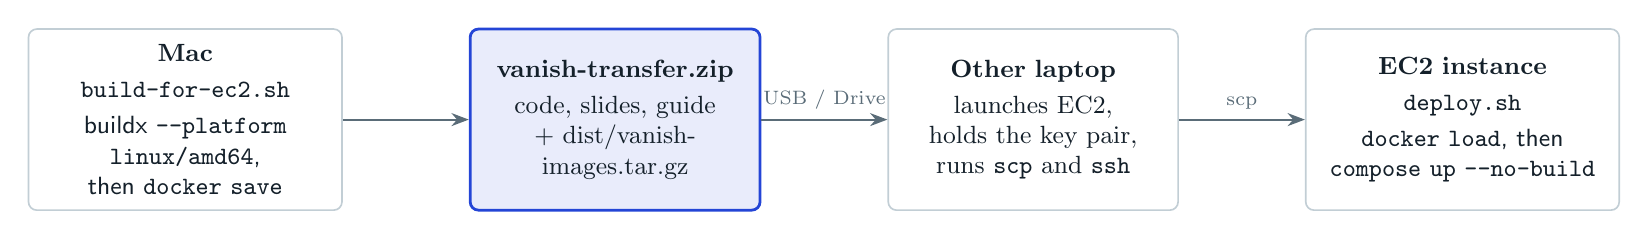
\begin{tikzpicture}[node distance=1.6cm, every node/.append style={font=\normalsize}]
    \node[box, text width=3.7cm, minimum height=2.3cm] (mac) {\textbf{Mac}\\[2pt]\small\ttfamily build-for-ec2.sh\\[2pt]\rmfamily\sffamily buildx \texttt{-{}-platform linux/amd64}, then \texttt{docker save}};
    \node[hot, text width=3.4cm, minimum height=2.3cm, right=of mac] (zip) {\textbf{vanish-transfer.zip}\\[2pt]\small code, slides, guide\\+ dist/vanish-images.tar.gz};
    \node[box, text width=3.4cm, minimum height=2.3cm, right=of zip] (pc) {\textbf{Other laptop}\\[2pt]\small launches EC2, holds the key pair, runs \texttt{scp} and \texttt{ssh}};
    \node[box, text width=3.7cm, minimum height=2.3cm, right=of pc] (ec2) {\textbf{EC2 instance}\\[2pt]\small\ttfamily deploy.sh\\[2pt]\rmfamily\sffamily \texttt{docker load}, then \texttt{compose up -{}-no-build}};
    \draw[arr] (mac) -- (zip);
    \draw[arr] (zip) -- node[lbl, above] {USB / Drive} (pc);
    \draw[arr] (pc) -- node[lbl, above] {scp} (ec2);
  \end{tikzpicture}}
  \vspace{0.9em}

  \begin{alertblock}{Why \texttt{linux/amd64}?}
    \small Apple Silicon Macs build \texttt{arm64} images by default, but a t3.micro has an Intel/AMD processor. A wrong image fails with \emph{exec format error}, so \code{deploy.sh} checks the architecture before starting.
  \end{alertblock}
\end{frame}
\note{[C] We build the images once and ship them. On the Mac, one script builds the app image for linux/amd64, downloads Caddy, and saves both into a single archive inside the project zip. We carry that zip to the laptop we deploy from, copy it to EC2 with scp, and our deploy script loads the images and starts them, with no build on the server. The platform flag matters: Apple Silicon builds arm64 by default, which won't run on a t3.micro, so the deploy script checks this before starting.}

% ===================================================================================== 16
\begin{frame}[fragile]{Deploying on EC2 in four steps}
  \begin{columns}[T]
    \column{0.46\textwidth}
    \begin{enumerate}\small
      \item \textbf{Launch} a t3.micro with Ubuntu 24.04, key pair \code{vanish-key}, HTTP + HTTPS open, SSH from our IP, and \code{user-data.sh} pasted in.
      \item \textbf{Copy} the zip with \code{scp}.
      \item \textbf{Unzip} and run \code{deploy.sh}.
      \item \textbf{Open} \code{https://<public-ip>}.
    \end{enumerate}
    \column{0.52\textwidth}
\begin{lstlisting}[language=bash]
# from the laptop
scp -i vanish-key.pem vanish-transfer.zip \
    ubuntu@13.233.45.67:~
ssh -i vanish-key.pem ubuntu@13.233.45.67

# on the instance
unzip vanish-transfer.zip && cd vanish
bash deploy/deploy.sh
docker compose ps
docker compose logs caddy   # certificate
\end{lstlisting}
  \end{columns}
  \vspace{0.3em}
  \muted{\small \code{deploy.sh} asks the instance metadata service for the public IP, writes it to \code{.env}, loads the images and starts both containers.}
\end{frame}
\note{[C] Deployment takes four steps. We launch a t3.micro with Ubuntu, open HTTP and HTTPS, restrict SSH to our IP, and paste our user-data script, which installs Docker at first boot. Then we copy the zip over with scp, log in with ssh, unzip it and run one script. It finds the public IP from the instance metadata service, loads the images, starts both containers, and Caddy obtains the certificate within a minute.}

% ===================================================================================== 17
\section{Results}
\begin{frame}{Security measures}
  \begin{columns}[T]
    \column{0.48\textwidth}
    \textbf{Data}
    \begin{itemize}\small
      \item Server stores ciphertext, timestamps and counters only
      \item Key in the URL fragment; removed from the address bar after opening
      \item Delete tokens stored as SHA-256 hashes
      \item Notes up to 4,000 characters; 20 new notes per minute per IP
    \end{itemize}
    \column{0.48\textwidth}
    \textbf{Infrastructure}
    \begin{itemize}\small
      \item Security group: only ports 22 (our IP), 80 and 443
      \item App port bound to localhost; only Caddy is public
      \item Container runs as a non-root user
      \item HTTPS everywhere, HSTS, strict Content-Security-Policy, no referrer
    \end{itemize}
  \end{columns}
\end{frame}
\note{[B] Security works in two layers. For data: the server only ever sees ciphertext, the key lives in the URL fragment and is removed from the address bar after opening, delete tokens are hashed, and note creation is rate-limited. For infrastructure: the security group exposes only three ports, the app container isn't directly reachable, it runs as a non-root user, and every response is served over HTTPS with strict browser security headers.}

% ===================================================================================== 18
\begin{frame}{Testing}
  \begin{columns}[T]
    \column{0.40\textwidth}
    \begin{block}{Automated tests (pytest)}
      \centering\vspace{2pt}
      {\Huge\bfseries\color{okgreen} 16 / 16}\\[2pt]
      \small passing
    \end{block}
    \small
    \begin{itemize}
      \item View counting and burn-on-last-view
      \item 8 concurrent opens: exactly 1 winner
      \item Expiry and cleanup, delete tokens
      \item Input validation, rate limit, pages
    \end{itemize}
    \column{0.56\textwidth}
    \textbf{Live checks on the EC2 deployment}
    \small
    \begin{enumerate}
      \item HTTPS loads; \code{http://} redirects to \code{https://}
      \item Create a 2-view note; open it twice; third open shows ``vanished''
      \item Wrong passphrase rejected; right one decrypts
      \item \emph{Destroy now} works; missing key detected
      \item Port 8000 unreachable from the internet
      \item Notes survive \code{docker compose restart}
      \item Database holds ciphertext only
    \end{enumerate}
  \end{columns}
\end{frame}
\note{[A] We tested at two levels. Sixteen automated tests run against the real Flask app and all pass, including the concurrency test. Then on the live EC2 instance we checked HTTPS and the redirect, the full view and burn cycle, the passphrase, early destroy, that port 8000 is closed to the internet, that notes survive a restart, and that the database only contains ciphertext.}

% ===================================================================================== 19
\begin{frame}{Cost}
  \begin{columns}[c]
    \column{0.58\textwidth}
    \small
    \begin{tabularx}{\linewidth}{@{}X r@{}}
      \toprule
      \textbf{Item (ap-south-1, 24/7)} & \textbf{USD / month} \\
      \midrule
      t3.micro instance (\$0.0112 / hour) & $\approx$ 8.20 \\
      Public IPv4 address               & $\approx$ 3.65 \\
      8 GiB gp3 EBS volume              & $\approx$ 0.75 \\
      \midrule
      \textbf{Total}                    & $\approx$ \textbf{12.60} \\
      \bottomrule
    \end{tabularx}
    \column{0.38\textwidth}
    \begin{exampleblock}{Paid by the Free plan}
      \small New AWS accounts get \textbf{\$100 credit}; t3.micro is Free Tier eligible. Our out-of-pocket cost: \textbf{INR 0}.
    \end{exampleblock}
    \vspace{0.3em}
    \muted{\small Stopping the instance when idle leaves only the disk charge.}
  \end{columns}
\end{frame}
\note{[C] Running all month, the instance, its public IP and its disk cost about twelve and a half dollars. New AWS accounts on the Free plan get a hundred dollars of credit and t3.micro is Free Tier eligible, so our out-of-pocket cost was zero. When we aren't using it, we stop the instance, and only the small disk charge remains.}

% ===================================================================================== 20
\section{Conclusion}
\begin{frame}{Challenges and lessons learned}
  \begin{itemize}
    \item \hl{CPU architecture matters.} Images built on an Apple Silicon Mac are \code{arm64}; EC2 t3 is \code{amd64}. Fixed with \code{buildx -{}-platform linux/amd64} and a check in \code{deploy.sh}.
    \item \hl{Browser crypto needs HTTPS.} Web Crypto is disabled on plain \code{http://}, so Caddy with a Let's Encrypt IP certificate is part of the design.
    \item \hl{Public IPs change.} Stopping and starting the instance gives a new IP; re-running \code{deploy.sh} picks it up automatically.
    \item \hl{1 GiB of RAM is tight.} User data adds 1 GiB of swap so builds on the instance never run out of memory.
  \end{itemize}
\end{frame}
\note{[B] We learned a few things the hard way. CPU architecture matters: images from an Apple Silicon Mac won't run on an Intel EC2 instance unless you build for linux/amd64. Browser encryption requires HTTPS, so getting a certificate without a domain became part of the design. Public IPs change when you stop an instance, so the deploy script re-detects it. And a one-gigabyte instance needs swap to build images safely.}

% ===================================================================================== 21
\begin{frame}{Limitations and future work}
  \begin{columns}[T]
    \column{0.47\textwidth}
    \textbf{Limitations}
    \begin{itemize}\small
      \item Anyone holding the full link can read the note; use a passphrase for sensitive data
      \item One instance: no redundancy if it stops
      \item SQLite on one disk: fine for this scale, not for many servers
    \end{itemize}
    \column{0.49\textwidth}
    \textbf{Future work}
    \begin{itemize}\small
      \item Custom domain and an Elastic IP for a stable address
      \item Managed database (Amazon RDS) and two instances behind a load balancer
      \item Image registry (Amazon ECR) and a CI pipeline for builds
      \item File attachments, encrypted the same way
    \end{itemize}
  \end{columns}
\end{frame}
\note{[B] Some honest limits. Anyone with the full link can read the note, so sensitive notes should use a passphrase. One instance means no redundancy, and SQLite suits a single server. Next steps would be a custom domain with a stable Elastic IP, a managed database with two instances behind a load balancer, a container registry with automated builds, and encrypted file attachments.}

% ===================================================================================== 22
\begin{frame}{Summary}
  \begin{columns}[c]
    \column{0.62\textwidth}
    \begin{itemize}
      \item Secrets that \hl{self-destruct} after N views or T time
      \item \hl{Zero-knowledge}: encrypted in the browser, ciphertext on the server
      \item \hl{Atomic} view counting, verified under concurrency
      \item Packaged as \hl{Docker images}, run with Docker Compose
      \item Deployed on \hl{Amazon EC2} over HTTPS, for INR 0
    \end{itemize}
    \column{0.34\textwidth}
    \centering
    {\Large\bfseries Thank you}\\[6pt]
    \muted{Questions?}\\[14pt]
    \small \memberA\\\memberB\\\memberC
  \end{columns}
\end{frame}
\note{[B] To sum up: Vanish lets you share a secret that destroys itself, it never sees your data in plain text, its view limits hold under concurrent access, and the whole thing is packaged with Docker and running on Amazon EC2 over HTTPS, at no cost to us. Thank you for watching.}

\end{document}
"
%  On Overleaf: upload this folder (with img/), set the compiler to pdfLaTeX.
%  For the notes version on Overleaf, uncomment the next line:
% \def\withnotes{}
%
%  Edit the names, college and course in the "EDIT ME" block below.
% =====================================================================================
\documentclass[aspectratio=169,11pt]{beamer}

\usetheme[progressbar=frametitle, numbering=fraction, sectionpage=none, block=fill]{metropolis}

% ---------- fonts: Fira Sans if installed (Overleaf has it), otherwise Helvetica ----------
\usepackage[T1]{fontenc}
\IfFileExists{FiraSans.sty}{%
  \usepackage[sfdefault,scale=0.95]{FiraSans}%
  \usepackage[scale=0.85]{FiraMono}%
}{%
  \usepackage{lmodern}%
  \usepackage[scaled=0.92]{helvet}%
}

\usepackage{tikz}
\usetikzlibrary{positioning, fit, arrows.meta, backgrounds, calc, decorations.pathreplacing, shapes.geometric}
\usepackage{booktabs}
\usepackage{tabularx}
\usepackage{listings}
\usepackage{graphicx}

% ---------- EDIT ME ----------
\newcommand{\memberA}{Member A}
\newcommand{\memberB}{Member B}
\newcommand{\memberC}{Member C}
\newcommand{\college}{Your College Name}
\newcommand{\course}{Cloud Computing Project}
% -----------------------------

% ---------- colours (same palette as the app) ----------
\definecolor{ink}{HTML}{14202A}
\definecolor{mist}{HTML}{5A6C78}
\definecolor{fog}{HTML}{DDE6EB}
\definecolor{glass}{HTML}{F4F7F9}
\definecolor{line}{HTML}{C2CED5}
\definecolor{cobalt}{HTML}{2445D6}
\definecolor{ember}{HTML}{B23A12}
\definecolor{okgreen}{HTML}{1F6F4A}

\setbeamercolor{normal text}{fg=ink, bg=white}
\setbeamercolor{palette primary}{fg=white, bg=ink}
\setbeamercolor{frametitle}{fg=white, bg=ink}
\setbeamercolor{progress bar}{fg=cobalt, bg=fog}
\setbeamercolor{title separator}{fg=cobalt}
\setbeamercolor{alerted text}{fg=ember}
\setbeamercolor{example text}{fg=okgreen}
\setbeamercolor{block title}{fg=ink, bg=fog}
\setbeamercolor{block body}{fg=ink, bg=glass}
\setbeamercolor{itemize item}{fg=cobalt}
\setbeamercolor{enumerate item}{fg=cobalt}
\setbeamercolor{footline}{fg=mist}
\setbeamerfont{frametitle}{size=\large, series=\bfseries}
\setbeamerfont{note page}{size=\normalsize}
\setbeamertemplate{itemize items}{\raisebox{0.15ex}{\scriptsize$\blacktriangleright$}}

\newcommand{\hl}[1]{\textcolor{cobalt}{\textbf{#1}}}
\newcommand{\muted}[1]{\textcolor{mist}{#1}}
\newcommand{\code}[1]{{\ttfamily\small #1}}

% ---------- code listings ----------
\lstdefinelanguage{Docker}{
  morekeywords={FROM,ENV,WORKDIR,COPY,RUN,USER,EXPOSE,HEALTHCHECK,CMD},
  morecomment=[l]{\#}, morestring=[b]"}
\lstdefinelanguage{yaml}{
  morekeywords={services,image,build,restart,volumes,ports,environment,depends_on},
  morecomment=[l]{\#}, morestring=[b]"}
\lstset{
  basicstyle=\ttfamily\scriptsize\color{ink},
  keywordstyle=\color{cobalt}\bfseries,
  commentstyle=\color{mist}\itshape,
  stringstyle=\color{okgreen},
  backgroundcolor=\color{glass},
  frame=single, rulecolor=\color{line}, framesep=4pt, xleftmargin=4pt, xrightmargin=4pt,
  columns=fullflexible, keepspaces=true, showstringspaces=false,
  breaklines=true, aboveskip=2pt, belowskip=2pt, upquote=true
}

% ---------- TikZ styles ----------
\tikzset{
  >={Stealth[length=2.2mm]},
  box/.style={draw=line, line width=0.6pt, rounded corners=3pt, fill=white, align=center,
              inner sep=4pt, font=\small, text=ink},
  hot/.style={box, draw=cobalt, line width=1pt, fill=cobalt!10},
  group/.style={draw=line, line width=0.6pt, rounded corners=4pt, inner sep=7pt},
  arr/.style={->, draw=mist, line width=0.8pt},
  lbl/.style={font=\scriptsize, text=mist},
  flowstep/.style={box, minimum height=1.25cm, text width=2.15cm}
}

% ---------- speaker notes ----------
\ifdefined\withnotes
  \setbeameroption{show only notes}
  \setbeamertemplate{note page}{%
    \vspace{0.3cm}%
    \begin{minipage}[t]{0.36\paperwidth}\insertslideintonotes{0.33}\end{minipage}\hfill
    \begin{minipage}[t]{0.58\paperwidth}\raggedright\normalsize\insertnote\end{minipage}%
  }
\fi

\title{Vanish}
\subtitle{Self-destructing secret notes, containerised with Docker\\and deployed on Amazon EC2}
\author{\memberA \quad\textperiodcentered\quad \memberB \quad\textperiodcentered\quad \memberC}
\institute{\course, \college}
\date{November 2026}
\hypersetup{pdftitle={Vanish: self-destructing secret notes on Amazon EC2}, pdfauthor={\memberA, \memberB, \memberC}}

\begin{document}

% ===================================================================================== 1
\maketitle
\note{[A] Hi, we are \memberA, \memberB\ and \memberC. Our cloud computing project is Vanish: a web app for sharing a secret that deletes itself. We packaged it with Docker and deployed it on an Amazon EC2 virtual machine. In the next ten minutes we'll cover the problem, the design, a demo, how we deployed it, and what we learned.}

% ===================================================================================== 2
\begin{frame}{Agenda}
  \begin{columns}[T]
    \column{0.48\textwidth}
    \begin{enumerate}
      \item The problem and our objectives
      \item What Vanish does: a short demo
      \item Architecture on Amazon EC2
      \item Implementation: encryption, backend
    \end{enumerate}
    \column{0.48\textwidth}
    \begin{enumerate}\setcounter{enumi}{4}
      \item Docker, Docker Compose and Caddy
      \item Building and deploying to EC2
      \item Testing, security and cost
      \item Lessons learned and future work
    \end{enumerate}
  \end{columns}
\end{frame}
\note{[A] Here is our agenda. First the problem and our objectives, then what the app does with real screenshots. \memberC\ will explain the architecture on EC2, \memberA\ and \memberB\ the implementation, and then \memberC\ shows how we containerised and deployed it. We finish with testing, security, cost, and lessons learned.}

% ===================================================================================== 3
\section{Problem and objectives}
\begin{frame}{The problem: secrets live forever in chat history}
  \begin{columns}[c]
    \column{0.52\textwidth}
    \begin{itemize}
      \item We share passwords, Wi-Fi keys and API keys over WhatsApp, email and Slack.
      \item Those messages stay in history, cloud backups and screenshots \hl{indefinitely}.
      \item Existing ``secret sharing'' sites ask you to \alert{trust their server} with the plain text.
    \end{itemize}
    \vspace{0.4em}
    \muted{\small A secret should be readable once, by the right person, and then disappear.}
    \column{0.44\textwidth}
    \centering
    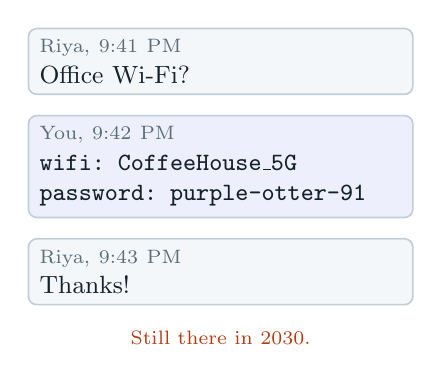
\begin{tikzpicture}[font=\small]
      \node[box, text width=4.6cm, align=left, fill=glass] (c1) {\muted{\scriptsize Riya, 9:41 PM}\\Office Wi-Fi?};
      \node[box, text width=4.6cm, align=left, fill=cobalt!8, below=0.25cm of c1] (c2)
        {\muted{\scriptsize You, 9:42 PM}\\\ttfamily wifi: CoffeeHouse\_5G\\password: purple-otter-91};
      \node[box, text width=4.6cm, align=left, fill=glass, below=0.25cm of c2] (c3) {\muted{\scriptsize Riya, 9:43 PM}\\Thanks!};
      \node[lbl, below=0.2cm of c3, text=ember] {Still there in 2030.};
    \end{tikzpicture}
  \end{columns}
\end{frame}
\note{[A] Think about the last time you sent someone a password. It's probably still sitting in that chat, in cloud backups, maybe in a screenshot. Messages last forever, but secrets shouldn't. And the websites that offer one-time links usually receive your secret in plain text, so you have to trust them completely.}

% ===================================================================================== 4
\begin{frame}{Objectives}
  \begin{enumerate}
    \item \hl{Self-destruct}: a note expires after \emph{N} views or \emph{T} time, whichever comes first.
    \item \hl{Zero knowledge}: the server stores only ciphertext and can never read a note.
    \item \hl{Correct under load}: two people can never both get the last view.
    \item \hl{Containerised}: the whole app runs from Docker images with one command.
    \item \hl{Deployed on a public cloud}: one Amazon EC2 instance, served over HTTPS.
  \end{enumerate}
\end{frame}
\note{[A] We set five objectives. Notes must self-destruct after a number of views or a time limit. The server must never be able to read them. The view limit must hold even when two people open the link at the same moment. The app must be fully containerised. And it must run on a public cloud, Amazon EC2, over HTTPS.}

% ===================================================================================== 5
\section{What Vanish does}
\begin{frame}{How it works for a user}
  \centering
  
\begin{tikzpicture}[node distance=0.55cm]
    \node[flowstep] (s1) {\textbf{Write}\\\scriptsize paste the secret, pick views and expiry};
    \node[flowstep, hot, right=of s1] (s2) {\textbf{Encrypt}\\\scriptsize AES-256-GCM, in the browser};
    \node[flowstep, right=of s2] (s3) {\textbf{Share}\\\scriptsize link with the key after \#, plus QR code};
    \node[flowstep, right=of s3] (s4) {\textbf{Open}\\\scriptsize one view used, decrypted on the device};
    \node[flowstep, right=of s4, draw=ember, text=ember] (s5) {\textbf{Gone}\\\scriptsize deleted at the last view or expiry};
    \foreach \a/\b in {s1/s2, s2/s3, s3/s4, s4/s5} \draw[arr] (\a) -- (\b);
  \end{tikzpicture}
  \vspace{1em}

  \begin{columns}[T]
    \column{0.3\textwidth}\centering \hl{1 to 10} views\\\muted{\small chosen by the sender}
    \column{0.3\textwidth}\centering \hl{5 min to 7 days}\\\muted{\small whichever limit comes first}
    \column{0.3\textwidth}\centering \hl{Optional passphrase}\\\muted{\small a second layer of encryption}
  \end{columns}
\end{frame}
\note{[B] Here's the flow. You write a secret and choose a view limit and an expiry. Your browser encrypts it with AES-256 before anything is sent. You get a link and a QR code. When the recipient opens it, one view is used and the note is decrypted on their device. At the last view, or when time runs out, it's gone for good. You can also add a passphrase as a second lock.}

% ===================================================================================== 6
\begin{frame}{Demo: creating a secret}
  \begin{columns}[T]
    \column{0.49\textwidth}\centering
    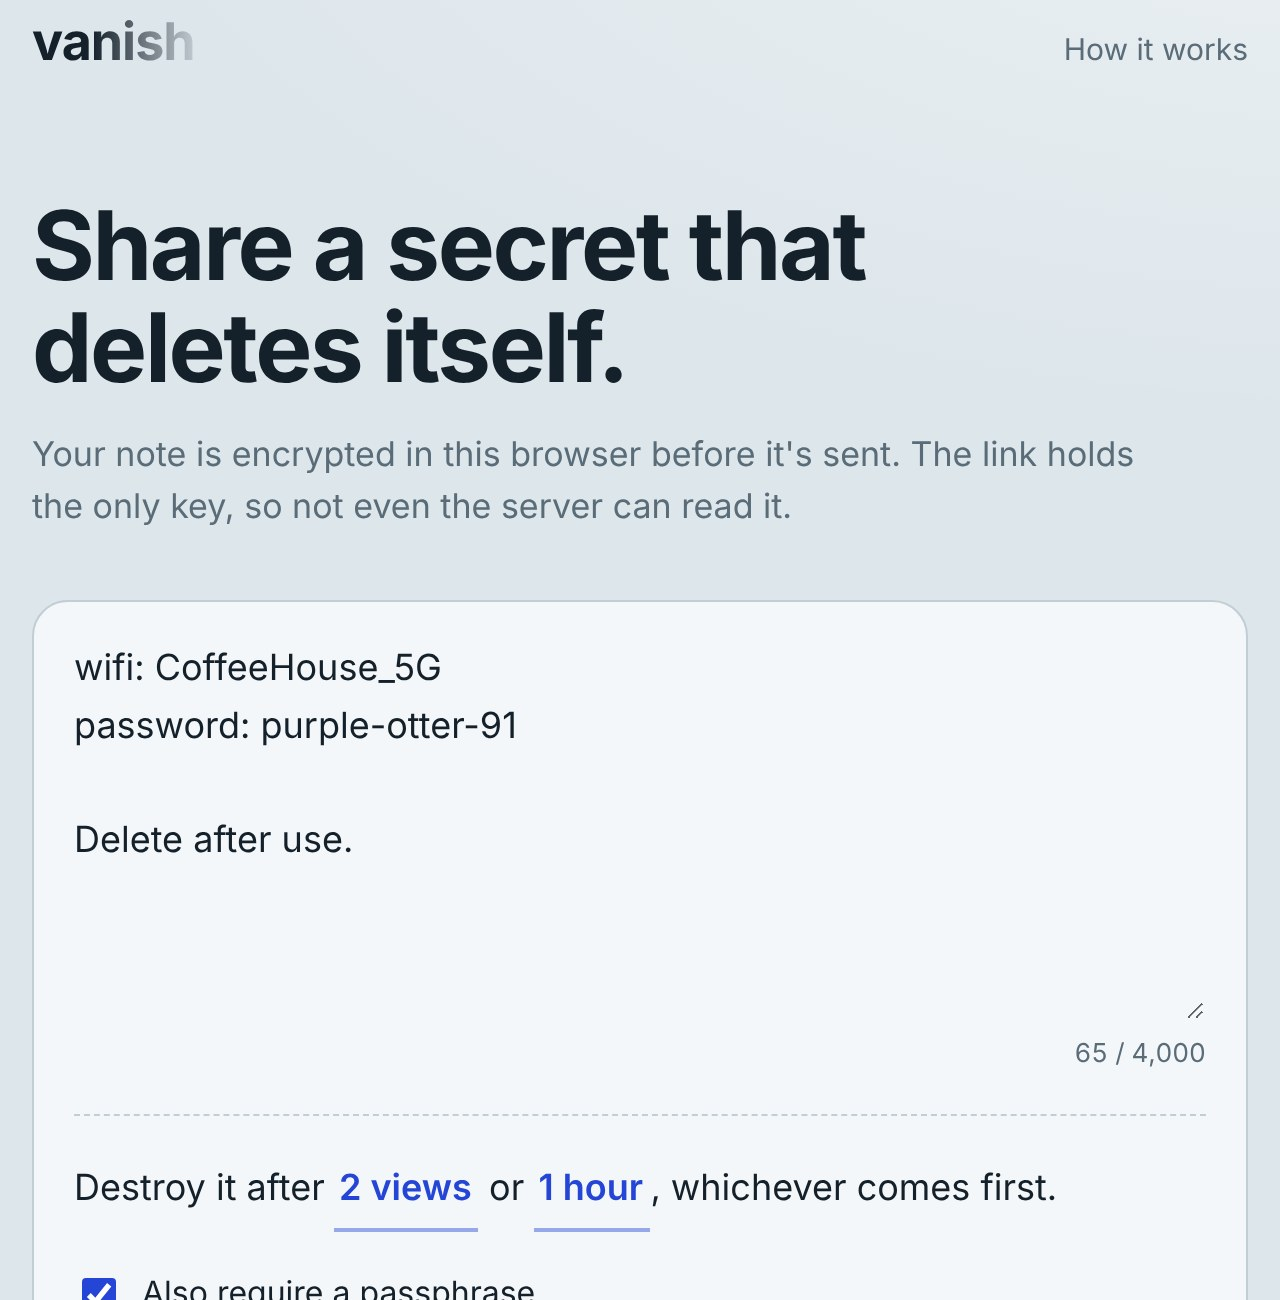
\includegraphics[width=0.84\linewidth]{img/create.jpg}\\[2pt]
    \muted{\scriptsize Write the note; 2 views or 1 hour; passphrase on}
    \column{0.49\textwidth}\centering
    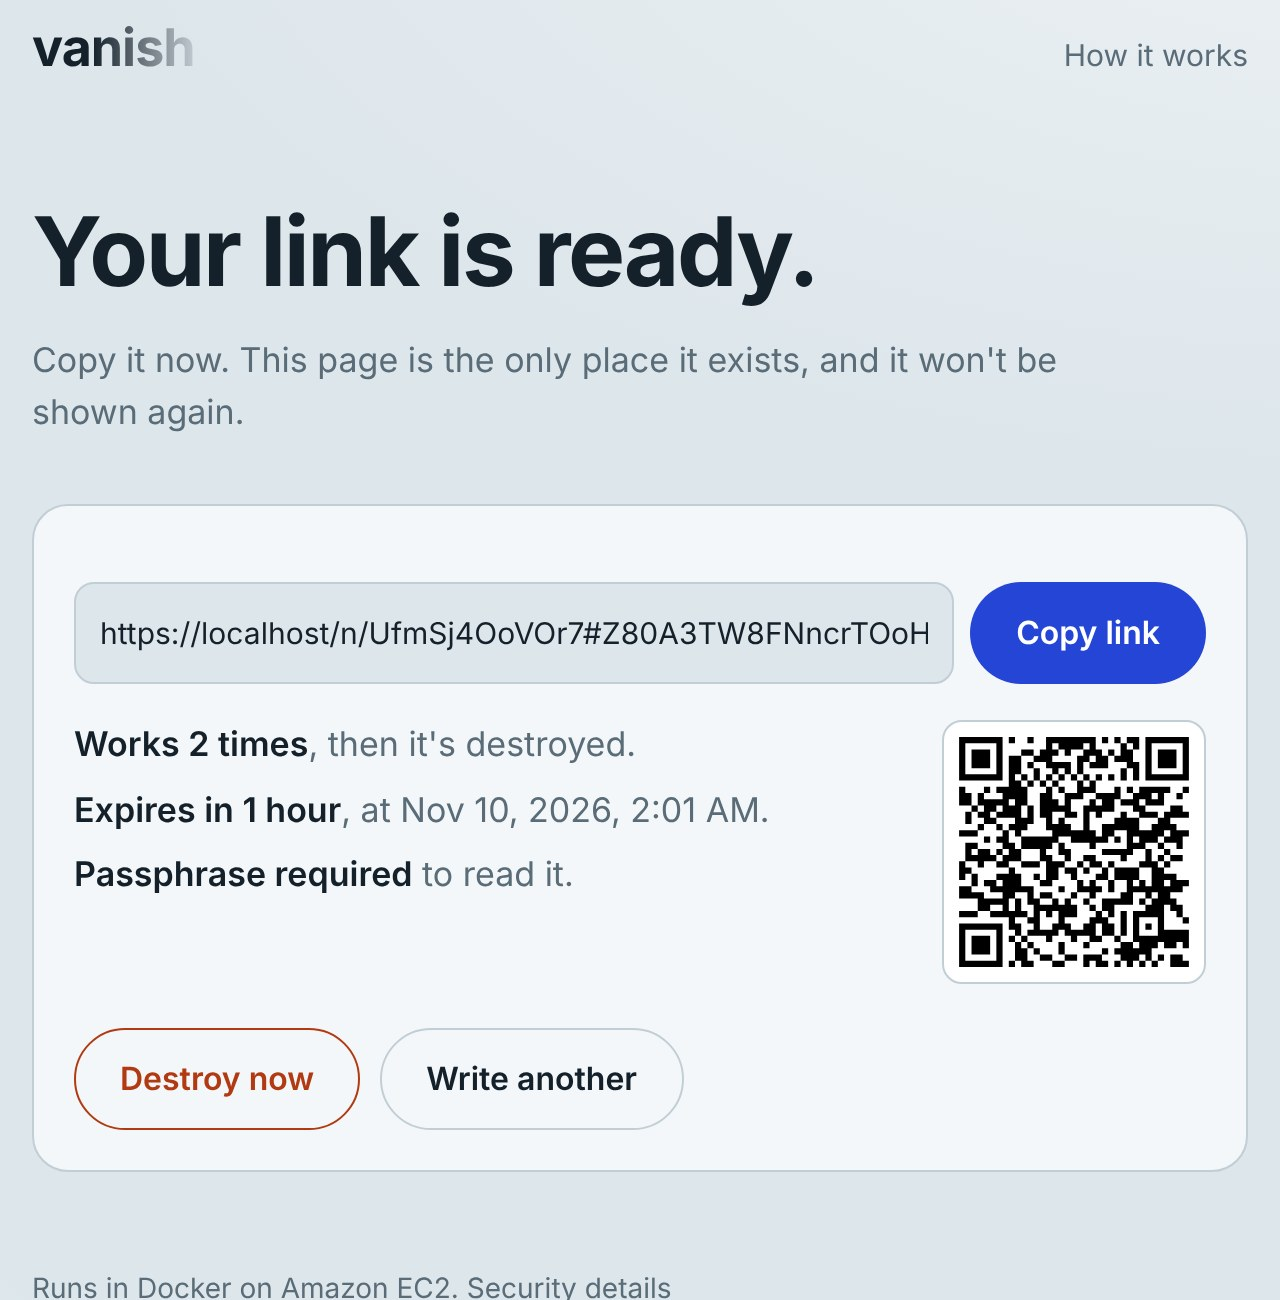
\includegraphics[width=0.84\linewidth]{img/link.jpg}\\[2pt]
    \muted{\scriptsize Encrypted in the browser; link and QR code returned}
  \end{columns}
\end{frame}
\note{[B] This is the app. I paste our café Wi-Fi password, choose two views or one hour, and add the passphrase ``mango''. When I press Create secret link, the text dissolves: it's being encrypted right here in the browser. On the right is the result: the link, a QR code for phones, and a summary of the rules. Only scrambled bytes were sent to the server.}

% ===================================================================================== 7
\begin{frame}{Demo: receiving it, then it vanishes}
  \begin{columns}[T]
    \column{0.32\textwidth}\centering
    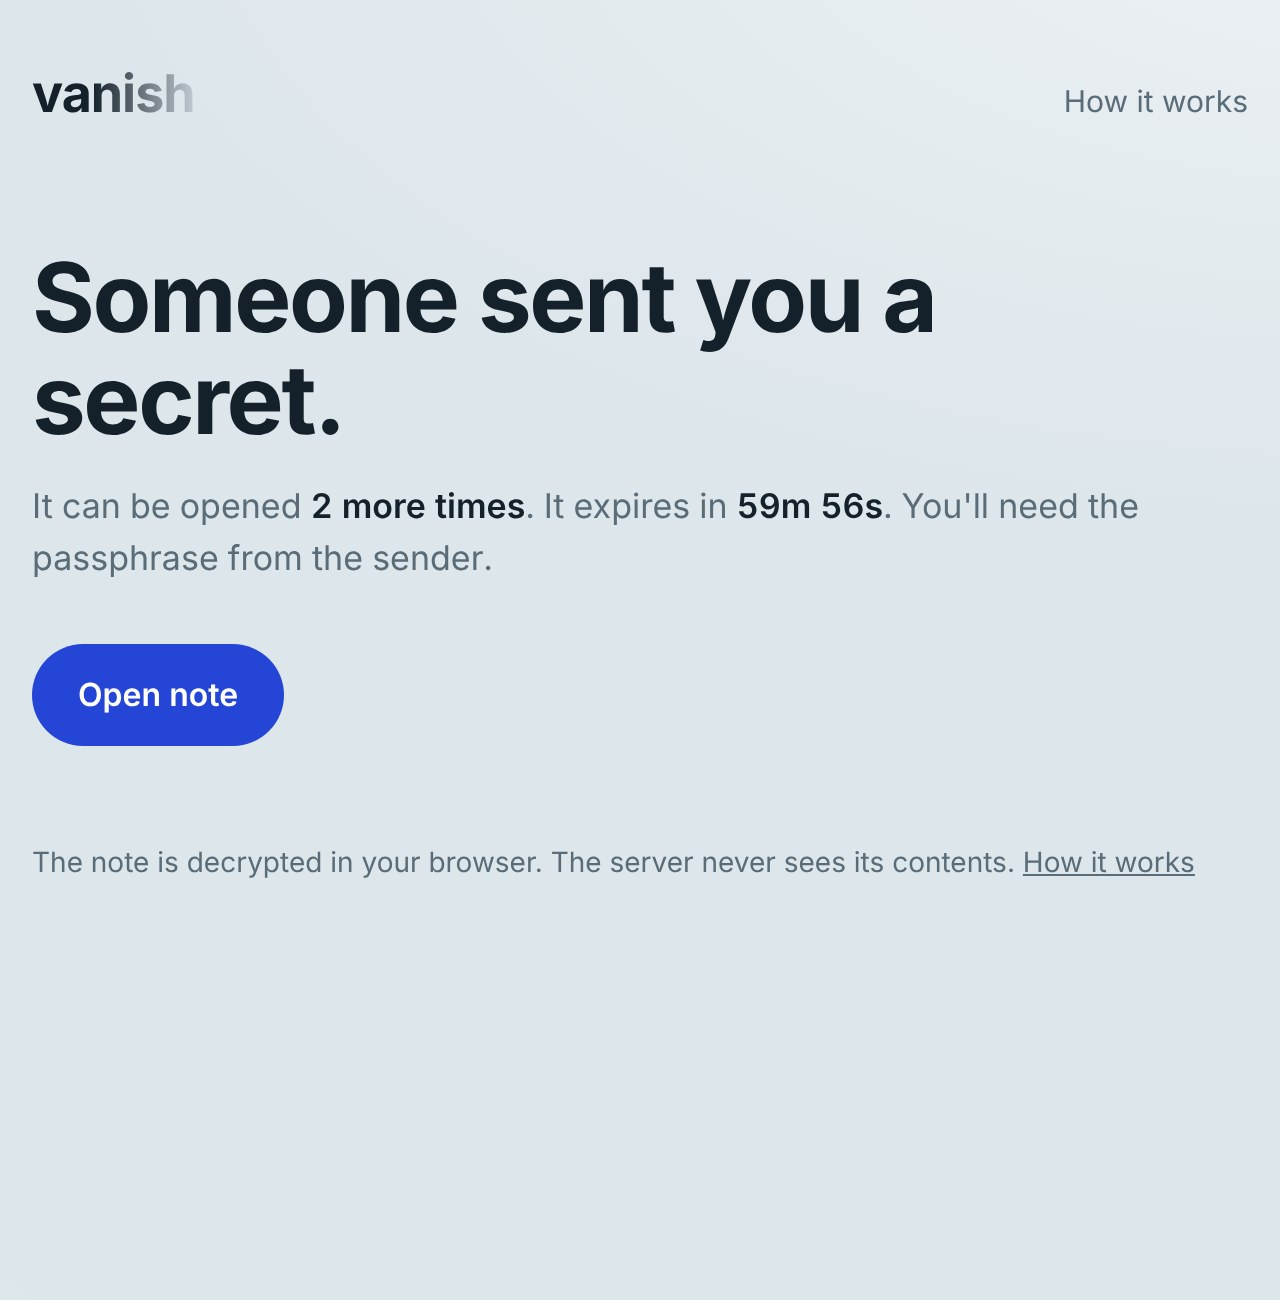
\includegraphics[width=\linewidth]{img/ready.jpg}\\[2pt]
    \muted{\scriptsize Countdown; opening the page uses no view}
    \column{0.32\textwidth}\centering
    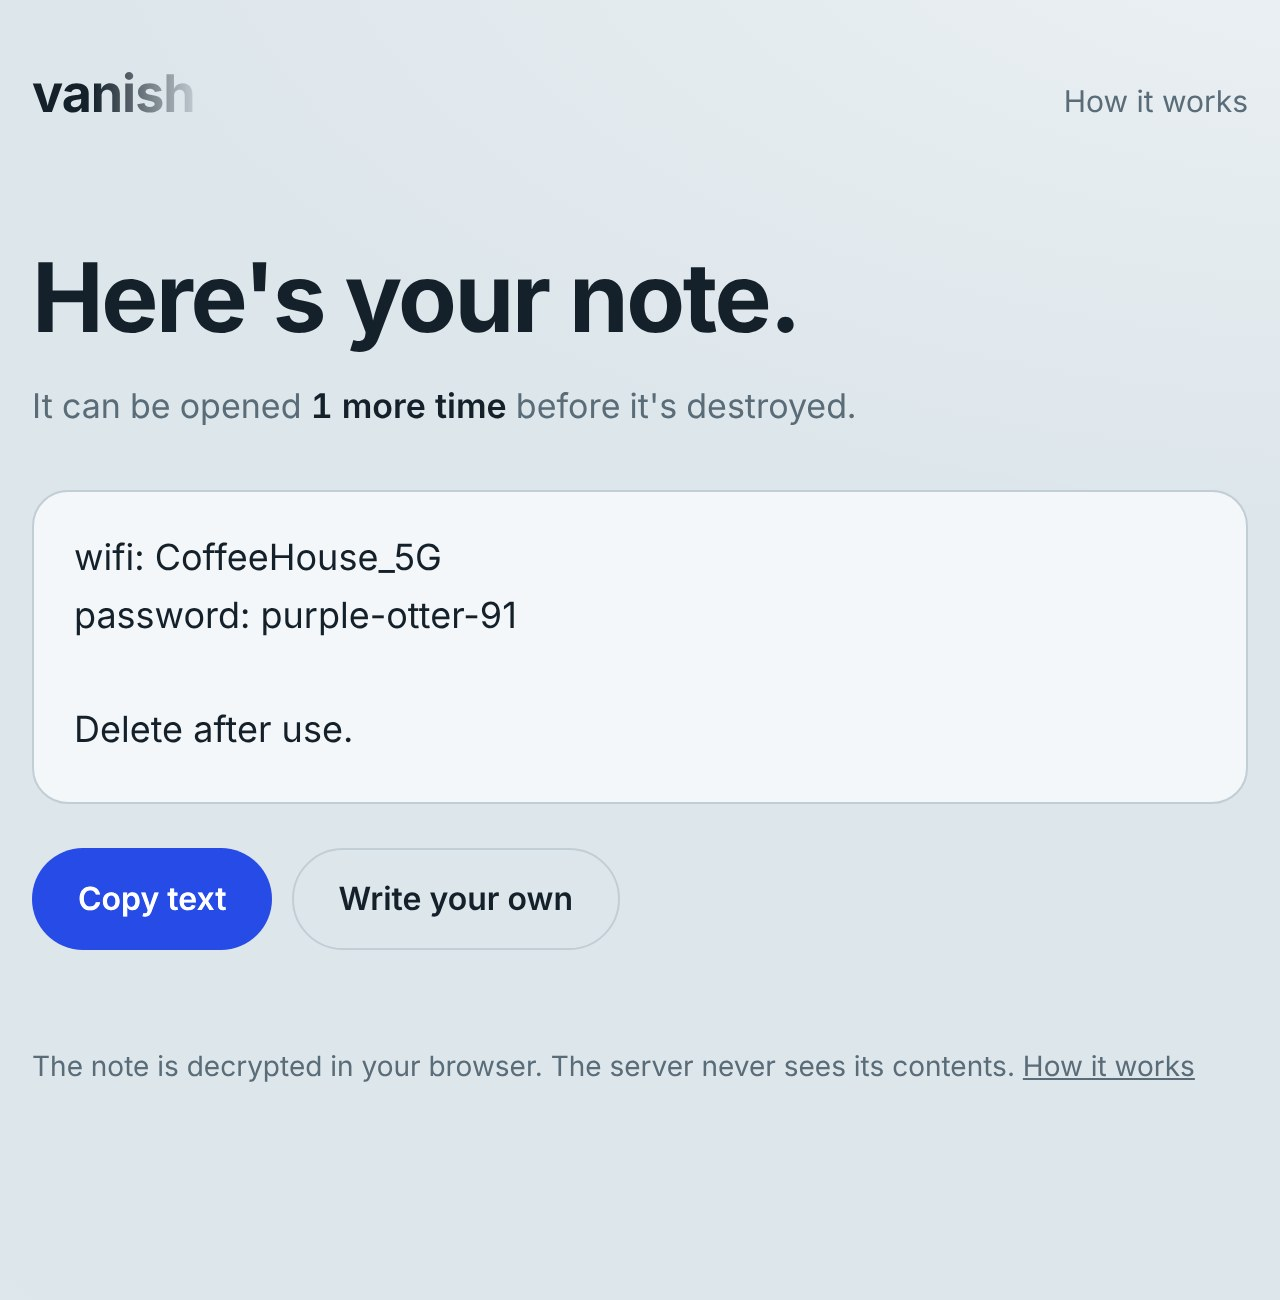
\includegraphics[width=\linewidth]{img/note.jpg}\\[2pt]
    \muted{\scriptsize Decrypted on the recipient's device}
    \column{0.32\textwidth}\centering
    
\includegraphics[width=\linewidth]{img/gone.jpg}\\[2pt]
    \muted{\scriptsize After the last view: nothing left}
  \end{columns}
\end{frame}
\note{[B] The recipient sees that a secret is waiting, how many views remain and a live countdown. Loading this page doesn't use a view, so chat apps that preview links can't burn it by accident. After entering the passphrase, the note is decrypted on their device. Once the last view is used, the server deletes it, and anyone opening the link again sees ``This note has vanished.''}

% ===================================================================================== 8
\section{Architecture}
\begin{frame}{Architecture on Amazon EC2}
  \centering
  \resizebox{\textwidth}{!}{%
  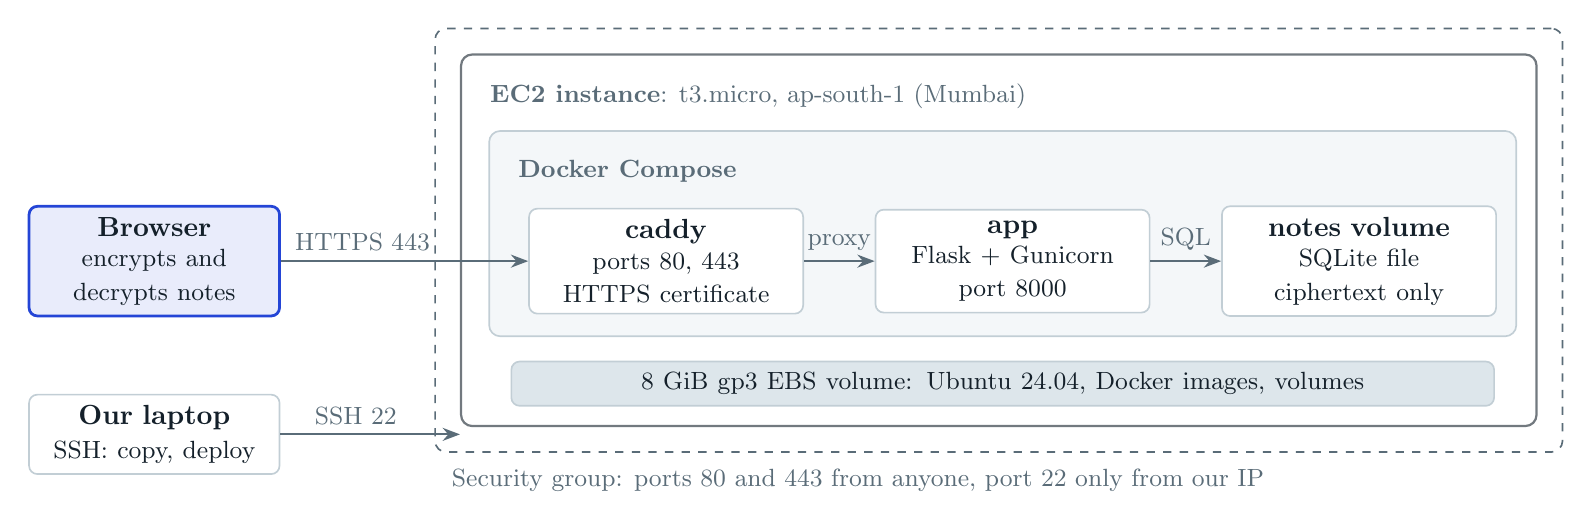
\begin{tikzpicture}[font=\normalsize, box/.append style={font=\normalsize}, hot/.append style={font=\normalsize}, lbl/.append style={font=\small}]
    \node[box, text width=3.2cm] (caddy) at (5.9,2.2) {\textbf{caddy}\\\small ports 80, 443\\HTTPS certificate};
    \node[box, text width=3.2cm] (app) at (10.3,2.2) {\textbf{app}\\\small Flask + Gunicorn\\port 8000};
    \node[box, text width=3.2cm] (vol) at (14.7,2.2) {\textbf{notes volume}\\\small SQLite file\\ciphertext only};
    \node[lbl, anchor=south west] (dcl) at ($(caddy.north west)+(-0.25,0.2)$) {\textbf{Docker Compose}};
    \begin{scope}[on background layer]
      \node[group, fill=glass, fit=(caddy)(app)(vol)(dcl)] (compose) {};
    \end{scope}
    \node[box, fill=fog, text width=12.2cm, anchor=north] (ebs) at ($(compose.south)+(0,-0.3)$)
      {\small 8 GiB gp3 EBS volume: Ubuntu 24.04, Docker images, volumes};
    \node[lbl, anchor=south west] (ecl) at ($(compose.north west)+(-0.1,0.15)$) {\textbf{EC2 instance}: t3.micro, ap-south-1 (Mumbai)};
    \begin{scope}[on background layer]
      \node[group, line width=0.8pt, draw=ink!60, fit=(compose)(ebs)(ecl)] (ec2) {};
      \node[group, dashed, draw=mist, inner sep=9pt, fit=(ec2)] (sg) {};
    \end{scope}
    \node[lbl, anchor=north west] at ($(sg.south west)+(0.1,-0.08)$) {Security group: ports 80 and 443 from anyone, port 22 only from our IP};
    \node[hot, text width=2.9cm] (browser) at (-0.6,2.2) {\textbf{Browser}\\\small encrypts and\\decrypts notes};
    \node[box, text width=2.9cm] (laptop) at (-0.6,0.0) {\textbf{Our laptop}\\\small SSH: copy, deploy};
    \draw[arr] (browser) -- node[lbl, above, pos=0.33] {HTTPS 443} (caddy);
    \draw[arr] (caddy) -- node[lbl, above] {proxy} (app);
    \draw[arr] (app) -- node[lbl, above] {SQL} (vol);
    \draw[arr] (laptop) -- node[lbl, above, pos=0.42] {SSH 22} (laptop -| ec2.west);
  \end{tikzpicture}}
\end{frame}
\note{[C] Everything runs on one Amazon EC2 virtual machine: a t3.micro running Ubuntu in the Mumbai region. A security group, AWS's firewall, lets anyone in on ports 80 and 443, but SSH only from our own IP. Inside, Docker Compose runs two containers. Caddy is the public web server: it gets a free HTTPS certificate and forwards requests to our app container, Flask with Gunicorn. The app keeps notes in a SQLite file on a Docker volume, which lives on the instance's EBS disk.}

% ===================================================================================== 9
\begin{frame}{Cloud services and features used}
  \small
  \begin{tabularx}{\textwidth}{@{}l X l@{}}
    \toprule
    \textbf{Service / feature} & \textbf{How Vanish uses it} & \textbf{Setting} \\
    \midrule
    EC2 instance        & Runs Docker and both containers                    & t3.micro, 2 vCPU, 1 GiB \\
    AMI                 & Operating system image                              & Ubuntu Server 24.04 LTS \\
    User data           & Installs Docker and swap on first boot              & \code{deploy/user-data.sh} \\
    Instance metadata   & \code{deploy.sh} looks up the public IP (IMDSv2)     & 169.254.169.254 \\
    Security group      & Stateful firewall in front of the instance          & 22 (our IP), 80, 443 \\
    Key pair            & Password-less SSH login                              & RSA, \code{.pem} \\
    EBS volume          & Disk for OS, images and the notes database          & 8 GiB gp3 \\
    Public IPv4         & Address users connect to; HTTPS certificate is for it & auto-assigned \\
    EC2 monitoring      & CPU, network and status checks                      & Monitoring tab \\
    \bottomrule
  \end{tabularx}
\end{frame}
\note{[C] These are the EC2 features we used. The instance type and the Ubuntu AMI. A user-data script that installs Docker automatically at first boot. The instance metadata service, which our deploy script queries for the public IP. A security group as the firewall, a key pair for SSH, an 8 GiB EBS volume for storage, the public IPv4 address, and EC2's built-in monitoring.}

% ===================================================================================== 10
\section{Implementation}
\begin{frame}{Zero-knowledge encryption: the key never reaches the server}
  \centering
  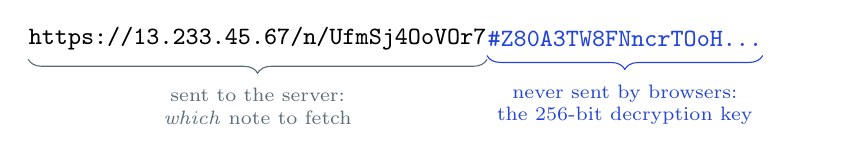
\begin{tikzpicture}
    \node[font=\ttfamily\small, inner sep=0] (a) {https://13.233.45.67/n/UfmSj4OoVOr7};
    \node[font=\ttfamily\small, inner sep=0, anchor=west, text=cobalt] (b) at (a.east) {\#Z80A3TW8FNncrTOoH\dots};
    \draw[decorate, decoration={brace, mirror, amplitude=5pt}, draw=mist] ([yshift=-3pt]a.south west) -- ([yshift=-3pt]a.south east)
      node[midway, below=7pt, lbl, text width=5.2cm, align=center] {sent to the server:\\\textit{which} note to fetch};
    \draw[decorate, decoration={brace, mirror, amplitude=5pt}, draw=cobalt] ([yshift=-3pt]b.south west) -- ([yshift=-3pt]b.south east)
      node[midway, below=7pt, font=\scriptsize, text=cobalt, text width=4.6cm, align=center] {never sent by browsers:\\the 256-bit decryption key};
  \end{tikzpicture}
  \vspace{0.8em}

  \begin{columns}[T]
    \column{0.48\textwidth}
    \begin{itemize}\small
      \item Browser generates a random 256-bit key and encrypts with \hl{AES-256-GCM} (Web Crypto API).
      \item Only \code{\{ciphertext, iv\}} is uploaded.
    \end{itemize}
    \column{0.48\textwidth}
    \begin{itemize}\small
      \item Optional passphrase: second layer, key from \hl{PBKDF2-SHA256}, 310,000 rounds.
      \item GCM is authenticated: tampered data fails to decrypt.
    \end{itemize}
  \end{columns}
\end{frame}
\note{[B] This is the core idea. The part of the link before the hash tells the server which note to fetch. The part after the hash is the 256-bit decryption key, and browsers never send that part to any server. So our EC2 instance only ever stores scrambled ciphertext. Encryption uses AES-256-GCM from the browser's built-in Web Crypto API, and the optional passphrase adds a second layer derived with PBKDF2.}

% ===================================================================================== 11
\begin{frame}{The API: five small endpoints}
  \small
  \begin{tabularx}{\textwidth}{@{}l l X@{}}
    \toprule
    \textbf{Method} & \textbf{Path} & \textbf{What it does} \\
    \midrule
    \code{POST}   & \code{/api/notes}             & Store \code{ciphertext}, \code{iv}, view limit (1--10), expiry (5 min--7 days) \\
    \code{GET}    & \code{/api/notes/\{id\}}      & Views left and expiry; \hl{does not use a view} (safe for link previews) \\
    \code{POST}   & \code{/api/notes/\{id\}/open} & Atomically use one view and return the ciphertext; \code{410 Gone} afterwards \\
    \code{DELETE} & \code{/api/notes/\{id\}}      & Destroy early with the secret delete token (stored as a SHA-256 hash) \\
    \code{GET}    & \code{/api/health}            & Liveness check used by the Docker health check \\
    \bottomrule
  \end{tabularx}
  \vspace{0.8em}

  \muted{A background thread deletes expired notes every 60 seconds; every read also checks the expiry time.}
\end{frame}
\note{[A] The backend is one Python file with five endpoints. Creating a note stores only ciphertext. Reading the metadata never uses a view, which is why WhatsApp previews can't burn a note. Opening uses one view atomically. There's an early-destroy endpoint protected by a secret token, and a health check that Docker uses. A background thread deletes expired notes every minute.}

% ===================================================================================== 12
\begin{frame}[fragile]{Atomic view counting: exactly one winner}
  \begin{columns}[T]
    \column{0.56\textwidth}
\begin{lstlisting}[language=SQL]
UPDATE notes
   SET view_count = view_count + 1
 WHERE id = ?
   AND view_count < max_views
   AND expires_at > ?
RETURNING ciphertext, iv, max_views,
          view_count, expires_at;
\end{lstlisting}
    \small\muted{From \code{open\_note} in \code{app/main.py}. If no row comes back, the API answers \code{410 Gone}.}
    \column{0.40\textwidth}
    \begin{block}{Why one statement?}
      \small
      Check and update happen together, so two people opening the \emph{last} view at the same moment can't both succeed.
    \end{block}
    \vspace{0.4em}
    \begin{exampleblock}{Tested}
      \small 8 simultaneous requests on a 1-view note: \textbf{1} gets the note, \textbf{7} get \code{410}.
    \end{exampleblock}
  \end{columns}
\end{frame}
\note{[A] The most important line of backend code is this single SQL statement. It increases the view count only if the note still has views left and hasn't expired, and returns the note in the same step. Because the check and the update are one atomic operation, two people can't both get the last view. Our test fires eight requests at the same moment at a one-view note: exactly one wins and seven get 410 Gone.}

% ===================================================================================== 13
\section{Docker and deployment}
\begin{frame}[fragile]{Containerising the app: the Dockerfile}
  \begin{columns}[T]
    \column{0.56\textwidth}
\begin{lstlisting}[language=Docker]
FROM python:3.13-slim
ENV DB_PATH=/data/vanish.db
WORKDIR /app
COPY requirements.txt .
RUN pip install --no-cache-dir \
        -r requirements.txt
COPY app/ .
RUN useradd --system --uid 10001 vanish \
 && mkdir -p /data \
 && chown vanish:vanish /data
USER vanish
EXPOSE 8000
HEALTHCHECK CMD python -c "..."  # GET /api/health
CMD ["gunicorn", "--bind", "0.0.0.0:8000",
     "--workers", "1", "--threads", "8",
     "main:app"]
\end{lstlisting}
    \column{0.40\textwidth}
    \begin{itemize}\small
      \item \hl{Slim base image}: small download, fewer packages to patch.
      \item \hl{Dependencies first}: code changes don't re-run \code{pip}.
      \item \hl{Non-root user}: a compromised app can't take over the container.
      \item \hl{Health check}: Docker flags the container if the API stops answering.
      \item \hl{Gunicorn}: production web server, 8 threads.
    \end{itemize}
  \end{columns}
\end{frame}
\note{[C] This is our Dockerfile. It starts from the official slim Python image, installs Flask and Gunicorn first so that code changes rebuild quickly, copies the app, and runs it as a non-root user. A health check calls our API every 30 seconds, and Gunicorn serves the app with eight threads.}

% ===================================================================================== 14
\begin{frame}[fragile]{Two containers: Docker Compose and Caddy}
  \begin{columns}[T]
    \column{0.55\textwidth}
    \small\textbf{compose.yaml} \muted{(abridged)}
\begin{lstlisting}[language=yaml]
services:
  app:
    image: vanish-app:1.0
    build: .
    volumes: ["notes:/data"]
    ports: ["127.0.0.1:8000:8000"]   # private
  caddy:
    image: caddy:2.11
    ports: ["80:80", "443:443"]       # public
    environment:
      SITE_ADDRESS: ${SITE_ADDRESS}
    volumes:
      - ./Caddyfile:/etc/caddy/Caddyfile:ro
      - caddy_data:/data
\end{lstlisting}
    \column{0.41\textwidth}
    \small\textbf{Caddyfile}
\begin{lstlisting}
{
  default_sni {$SITE_ADDRESS}
}
{$SITE_ADDRESS} {
  tls {
    issuer acme {
      profile shortlived
    }
  }
  encode zstd gzip
  reverse_proxy app:8000
}
\end{lstlisting}
    \small\muted{Free Let's Encrypt certificate for the public IP, renewed automatically.}
  \end{columns}
\end{frame}
\note{[C] Docker Compose runs two containers. The app's port is bound to localhost only, so the internet can reach it only through Caddy. Notes live in a named volume, so they survive restarts and rebuilds. On the right is the entire Caddyfile: it requests a free Let's Encrypt certificate for our IP address and forwards every request to the app. HTTPS isn't optional here: browsers only allow the Web Crypto API on secure pages.}

% ===================================================================================== 15
\begin{frame}{Build once, ship the image to EC2}
  \centering
  \resizebox{\textwidth}{!}{%
  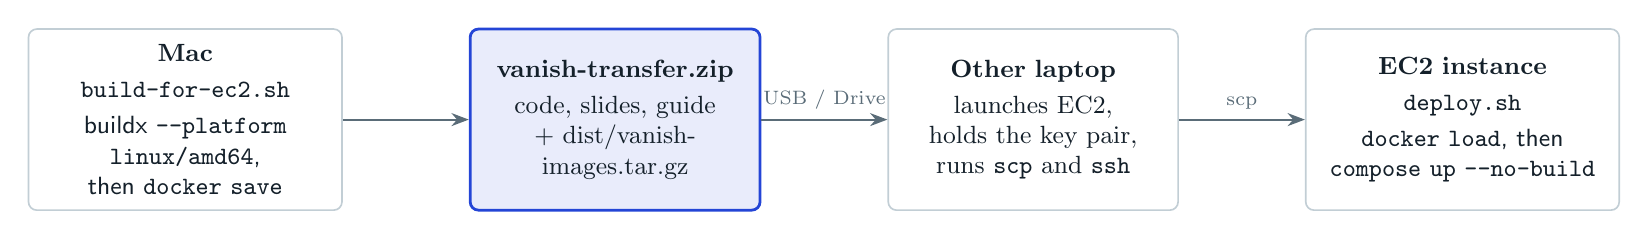
\begin{tikzpicture}[node distance=1.6cm, every node/.append style={font=\normalsize}]
    \node[box, text width=3.7cm, minimum height=2.3cm] (mac) {\textbf{Mac}\\[2pt]\small\ttfamily build-for-ec2.sh\\[2pt]\rmfamily\sffamily buildx \texttt{-{}-platform linux/amd64}, then \texttt{docker save}};
    \node[hot, text width=3.4cm, minimum height=2.3cm, right=of mac] (zip) {\textbf{vanish-transfer.zip}\\[2pt]\small code, slides, guide\\+ dist/vanish-images.tar.gz};
    \node[box, text width=3.4cm, minimum height=2.3cm, right=of zip] (pc) {\textbf{Other laptop}\\[2pt]\small launches EC2, holds the key pair, runs \texttt{scp} and \texttt{ssh}};
    \node[box, text width=3.7cm, minimum height=2.3cm, right=of pc] (ec2) {\textbf{EC2 instance}\\[2pt]\small\ttfamily deploy.sh\\[2pt]\rmfamily\sffamily \texttt{docker load}, then \texttt{compose up -{}-no-build}};
    \draw[arr] (mac) -- (zip);
    \draw[arr] (zip) -- node[lbl, above] {USB / Drive} (pc);
    \draw[arr] (pc) -- node[lbl, above] {scp} (ec2);
  \end{tikzpicture}}
  \vspace{0.9em}

  \begin{alertblock}{Why \texttt{linux/amd64}?}
    \small Apple Silicon Macs build \texttt{arm64} images by default, but a t3.micro has an Intel/AMD processor. A wrong image fails with \emph{exec format error}, so \code{deploy.sh} checks the architecture before starting.
  \end{alertblock}
\end{frame}
\note{[C] We build the images once and ship them. On the Mac, one script builds the app image for linux/amd64, downloads Caddy, and saves both into a single archive inside the project zip. We carry that zip to the laptop we deploy from, copy it to EC2 with scp, and our deploy script loads the images and starts them, with no build on the server. The platform flag matters: Apple Silicon builds arm64 by default, which won't run on a t3.micro, so the deploy script checks this before starting.}

% ===================================================================================== 16
\begin{frame}[fragile]{Deploying on EC2 in four steps}
  \begin{columns}[T]
    \column{0.46\textwidth}
    \begin{enumerate}\small
      \item \textbf{Launch} a t3.micro with Ubuntu 24.04, key pair \code{vanish-key}, HTTP + HTTPS open, SSH from our IP, and \code{user-data.sh} pasted in.
      \item \textbf{Copy} the zip with \code{scp}.
      \item \textbf{Unzip} and run \code{deploy.sh}.
      \item \textbf{Open} \code{https://<public-ip>}.
    \end{enumerate}
    \column{0.52\textwidth}
\begin{lstlisting}[language=bash]
# from the laptop
scp -i vanish-key.pem vanish-transfer.zip \
    ubuntu@13.233.45.67:~
ssh -i vanish-key.pem ubuntu@13.233.45.67

# on the instance
unzip vanish-transfer.zip && cd vanish
bash deploy/deploy.sh
docker compose ps
docker compose logs caddy   # certificate
\end{lstlisting}
  \end{columns}
  \vspace{0.3em}
  \muted{\small \code{deploy.sh} asks the instance metadata service for the public IP, writes it to \code{.env}, loads the images and starts both containers.}
\end{frame}
\note{[C] Deployment takes four steps. We launch a t3.micro with Ubuntu, open HTTP and HTTPS, restrict SSH to our IP, and paste our user-data script, which installs Docker at first boot. Then we copy the zip over with scp, log in with ssh, unzip it and run one script. It finds the public IP from the instance metadata service, loads the images, starts both containers, and Caddy obtains the certificate within a minute.}

% ===================================================================================== 17
\section{Results}
\begin{frame}{Security measures}
  \begin{columns}[T]
    \column{0.48\textwidth}
    \textbf{Data}
    \begin{itemize}\small
      \item Server stores ciphertext, timestamps and counters only
      \item Key in the URL fragment; removed from the address bar after opening
      \item Delete tokens stored as SHA-256 hashes
      \item Notes up to 4,000 characters; 20 new notes per minute per IP
    \end{itemize}
    \column{0.48\textwidth}
    \textbf{Infrastructure}
    \begin{itemize}\small
      \item Security group: only ports 22 (our IP), 80 and 443
      \item App port bound to localhost; only Caddy is public
      \item Container runs as a non-root user
      \item HTTPS everywhere, HSTS, strict Content-Security-Policy, no referrer
    \end{itemize}
  \end{columns}
\end{frame}
\note{[B] Security works in two layers. For data: the server only ever sees ciphertext, the key lives in the URL fragment and is removed from the address bar after opening, delete tokens are hashed, and note creation is rate-limited. For infrastructure: the security group exposes only three ports, the app container isn't directly reachable, it runs as a non-root user, and every response is served over HTTPS with strict browser security headers.}

% ===================================================================================== 18
\begin{frame}{Testing}
  \begin{columns}[T]
    \column{0.40\textwidth}
    \begin{block}{Automated tests (pytest)}
      \centering\vspace{2pt}
      {\Huge\bfseries\color{okgreen} 16 / 16}\\[2pt]
      \small passing
    \end{block}
    \small
    \begin{itemize}
      \item View counting and burn-on-last-view
      \item 8 concurrent opens: exactly 1 winner
      \item Expiry and cleanup, delete tokens
      \item Input validation, rate limit, pages
    \end{itemize}
    \column{0.56\textwidth}
    \textbf{Live checks on the EC2 deployment}
    \small
    \begin{enumerate}
      \item HTTPS loads; \code{http://} redirects to \code{https://}
      \item Create a 2-view note; open it twice; third open shows ``vanished''
      \item Wrong passphrase rejected; right one decrypts
      \item \emph{Destroy now} works; missing key detected
      \item Port 8000 unreachable from the internet
      \item Notes survive \code{docker compose restart}
      \item Database holds ciphertext only
    \end{enumerate}
  \end{columns}
\end{frame}
\note{[A] We tested at two levels. Sixteen automated tests run against the real Flask app and all pass, including the concurrency test. Then on the live EC2 instance we checked HTTPS and the redirect, the full view and burn cycle, the passphrase, early destroy, that port 8000 is closed to the internet, that notes survive a restart, and that the database only contains ciphertext.}

% ===================================================================================== 19
\begin{frame}{Cost}
  \begin{columns}[c]
    \column{0.58\textwidth}
    \small
    \begin{tabularx}{\linewidth}{@{}X r@{}}
      \toprule
      \textbf{Item (ap-south-1, 24/7)} & \textbf{USD / month} \\
      \midrule
      t3.micro instance (\$0.0112 / hour) & $\approx$ 8.20 \\
      Public IPv4 address               & $\approx$ 3.65 \\
      8 GiB gp3 EBS volume              & $\approx$ 0.75 \\
      \midrule
      \textbf{Total}                    & $\approx$ \textbf{12.60} \\
      \bottomrule
    \end{tabularx}
    \column{0.38\textwidth}
    \begin{exampleblock}{Paid by the Free plan}
      \small New AWS accounts get \textbf{\$100 credit}; t3.micro is Free Tier eligible. Our out-of-pocket cost: \textbf{INR 0}.
    \end{exampleblock}
    \vspace{0.3em}
    \muted{\small Stopping the instance when idle leaves only the disk charge.}
  \end{columns}
\end{frame}
\note{[C] Running all month, the instance, its public IP and its disk cost about twelve and a half dollars. New AWS accounts on the Free plan get a hundred dollars of credit and t3.micro is Free Tier eligible, so our out-of-pocket cost was zero. When we aren't using it, we stop the instance, and only the small disk charge remains.}

% ===================================================================================== 20
\section{Conclusion}
\begin{frame}{Challenges and lessons learned}
  \begin{itemize}
    \item \hl{CPU architecture matters.} Images built on an Apple Silicon Mac are \code{arm64}; EC2 t3 is \code{amd64}. Fixed with \code{buildx -{}-platform linux/amd64} and a check in \code{deploy.sh}.
    \item \hl{Browser crypto needs HTTPS.} Web Crypto is disabled on plain \code{http://}, so Caddy with a Let's Encrypt IP certificate is part of the design.
    \item \hl{Public IPs change.} Stopping and starting the instance gives a new IP; re-running \code{deploy.sh} picks it up automatically.
    \item \hl{1 GiB of RAM is tight.} User data adds 1 GiB of swap so builds on the instance never run out of memory.
  \end{itemize}
\end{frame}
\note{[B] We learned a few things the hard way. CPU architecture matters: images from an Apple Silicon Mac won't run on an Intel EC2 instance unless you build for linux/amd64. Browser encryption requires HTTPS, so getting a certificate without a domain became part of the design. Public IPs change when you stop an instance, so the deploy script re-detects it. And a one-gigabyte instance needs swap to build images safely.}

% ===================================================================================== 21
\begin{frame}{Limitations and future work}
  \begin{columns}[T]
    \column{0.47\textwidth}
    \textbf{Limitations}
    \begin{itemize}\small
      \item Anyone holding the full link can read the note; use a passphrase for sensitive data
      \item One instance: no redundancy if it stops
      \item SQLite on one disk: fine for this scale, not for many servers
    \end{itemize}
    \column{0.49\textwidth}
    \textbf{Future work}
    \begin{itemize}\small
      \item Custom domain and an Elastic IP for a stable address
      \item Managed database (Amazon RDS) and two instances behind a load balancer
      \item Image registry (Amazon ECR) and a CI pipeline for builds
      \item File attachments, encrypted the same way
    \end{itemize}
  \end{columns}
\end{frame}
\note{[B] Some honest limits. Anyone with the full link can read the note, so sensitive notes should use a passphrase. One instance means no redundancy, and SQLite suits a single server. Next steps would be a custom domain with a stable Elastic IP, a managed database with two instances behind a load balancer, a container registry with automated builds, and encrypted file attachments.}

% ===================================================================================== 22
\begin{frame}{Summary}
  \begin{columns}[c]
    \column{0.62\textwidth}
    \begin{itemize}
      \item Secrets that \hl{self-destruct} after N views or T time
      \item \hl{Zero-knowledge}: encrypted in the browser, ciphertext on the server
      \item \hl{Atomic} view counting, verified under concurrency
      \item Packaged as \hl{Docker images}, run with Docker Compose
      \item Deployed on \hl{Amazon EC2} over HTTPS, for INR 0
    \end{itemize}
    \column{0.34\textwidth}
    \centering
    {\Large\bfseries Thank you}\\[6pt]
    \muted{Questions?}\\[14pt]
    \small \memberA\\\memberB\\\memberC
  \end{columns}
\end{frame}
\note{[B] To sum up: Vanish lets you share a secret that destroys itself, it never sees your data in plain text, its view limits hold under concurrent access, and the whole thing is packaged with Docker and running on Amazon EC2 over HTTPS, at no cost to us. Thank you for watching.}

\end{document}
"
%  On Overleaf: upload this folder (with img/), set the compiler to pdfLaTeX.
%  For the notes version on Overleaf, uncomment the next line:
% \def\withnotes{}
%
%  Edit the names, college and course in the "EDIT ME" block below.
% =====================================================================================
\documentclass[aspectratio=169,11pt]{beamer}

\usetheme[progressbar=frametitle, numbering=fraction, sectionpage=none, block=fill]{metropolis}

% ---------- fonts: Fira Sans if installed (Overleaf has it), otherwise Helvetica ----------
\usepackage[T1]{fontenc}
\IfFileExists{FiraSans.sty}{%
  \usepackage[sfdefault,scale=0.95]{FiraSans}%
  \usepackage[scale=0.85]{FiraMono}%
}{%
  \usepackage{lmodern}%
  \usepackage[scaled=0.92]{helvet}%
}

\usepackage{tikz}
\usetikzlibrary{positioning, fit, arrows.meta, backgrounds, calc, decorations.pathreplacing, shapes.geometric}
\usepackage{booktabs}
\usepackage{tabularx}
\usepackage{listings}
\usepackage{graphicx}

% ---------- EDIT ME ----------
\newcommand{\memberA}{Member A}
\newcommand{\memberB}{Member B}
\newcommand{\memberC}{Member C}
\newcommand{\college}{Your College Name}
\newcommand{\course}{Cloud Computing Project}
% -----------------------------

% ---------- colours (same palette as the app) ----------
\definecolor{ink}{HTML}{14202A}
\definecolor{mist}{HTML}{5A6C78}
\definecolor{fog}{HTML}{DDE6EB}
\definecolor{glass}{HTML}{F4F7F9}
\definecolor{line}{HTML}{C2CED5}
\definecolor{cobalt}{HTML}{2445D6}
\definecolor{ember}{HTML}{B23A12}
\definecolor{okgreen}{HTML}{1F6F4A}

\setbeamercolor{normal text}{fg=ink, bg=white}
\setbeamercolor{palette primary}{fg=white, bg=ink}
\setbeamercolor{frametitle}{fg=white, bg=ink}
\setbeamercolor{progress bar}{fg=cobalt, bg=fog}
\setbeamercolor{title separator}{fg=cobalt}
\setbeamercolor{alerted text}{fg=ember}
\setbeamercolor{example text}{fg=okgreen}
\setbeamercolor{block title}{fg=ink, bg=fog}
\setbeamercolor{block body}{fg=ink, bg=glass}
\setbeamercolor{itemize item}{fg=cobalt}
\setbeamercolor{enumerate item}{fg=cobalt}
\setbeamercolor{footline}{fg=mist}
\setbeamerfont{frametitle}{size=\large, series=\bfseries}
\setbeamerfont{note page}{size=\normalsize}
\setbeamertemplate{itemize items}{\raisebox{0.15ex}{\scriptsize$\blacktriangleright$}}

\newcommand{\hl}[1]{\textcolor{cobalt}{\textbf{#1}}}
\newcommand{\muted}[1]{\textcolor{mist}{#1}}
\newcommand{\code}[1]{{\ttfamily\small #1}}

% ---------- code listings ----------
\lstdefinelanguage{Docker}{
  morekeywords={FROM,ENV,WORKDIR,COPY,RUN,USER,EXPOSE,HEALTHCHECK,CMD},
  morecomment=[l]{\#}, morestring=[b]"}
\lstdefinelanguage{yaml}{
  morekeywords={services,image,build,restart,volumes,ports,environment,depends_on},
  morecomment=[l]{\#}, morestring=[b]"}
\lstset{
  basicstyle=\ttfamily\scriptsize\color{ink},
  keywordstyle=\color{cobalt}\bfseries,
  commentstyle=\color{mist}\itshape,
  stringstyle=\color{okgreen},
  backgroundcolor=\color{glass},
  frame=single, rulecolor=\color{line}, framesep=4pt, xleftmargin=4pt, xrightmargin=4pt,
  columns=fullflexible, keepspaces=true, showstringspaces=false,
  breaklines=true, aboveskip=2pt, belowskip=2pt, upquote=true
}

% ---------- TikZ styles ----------
\tikzset{
  >={Stealth[length=2.2mm]},
  box/.style={draw=line, line width=0.6pt, rounded corners=3pt, fill=white, align=center,
              inner sep=4pt, font=\small, text=ink},
  hot/.style={box, draw=cobalt, line width=1pt, fill=cobalt!10},
  group/.style={draw=line, line width=0.6pt, rounded corners=4pt, inner sep=7pt},
  arr/.style={->, draw=mist, line width=0.8pt},
  lbl/.style={font=\scriptsize, text=mist},
  flowstep/.style={box, minimum height=1.25cm, text width=2.15cm}
}

% ---------- speaker notes ----------
\ifdefined\withnotes
  \setbeameroption{show only notes}
  \setbeamertemplate{note page}{%
    \vspace{0.3cm}%
    \begin{minipage}[t]{0.36\paperwidth}\insertslideintonotes{0.33}\end{minipage}\hfill
    \begin{minipage}[t]{0.58\paperwidth}\raggedright\normalsize\insertnote\end{minipage}%
  }
\fi

\title{Vanish}
\subtitle{Self-destructing secret notes, containerised with Docker\\and deployed on Amazon EC2}
\author{\memberA \quad\textperiodcentered\quad \memberB \quad\textperiodcentered\quad \memberC}
\institute{\course, \college}
\date{November 2026}
\hypersetup{pdftitle={Vanish: self-destructing secret notes on Amazon EC2}, pdfauthor={\memberA, \memberB, \memberC}}

\begin{document}

% ===================================================================================== 1
\maketitle
\note{[A] Hi, we are \memberA, \memberB\ and \memberC. Our cloud computing project is Vanish: a web app for sharing a secret that deletes itself. We packaged it with Docker and deployed it on an Amazon EC2 virtual machine. In the next ten minutes we'll cover the problem, the design, a demo, how we deployed it, and what we learned.}

% ===================================================================================== 2
\begin{frame}{Agenda}
  \begin{columns}[T]
    \column{0.48\textwidth}
    \begin{enumerate}
      \item The problem and our objectives
      \item What Vanish does: a short demo
      \item Architecture on Amazon EC2
      \item Implementation: encryption, backend
    \end{enumerate}
    \column{0.48\textwidth}
    \begin{enumerate}\setcounter{enumi}{4}
      \item Docker, Docker Compose and Caddy
      \item Building and deploying to EC2
      \item Testing, security and cost
      \item Lessons learned and future work
    \end{enumerate}
  \end{columns}
\end{frame}
\note{[A] Here is our agenda. First the problem and our objectives, then what the app does with real screenshots. \memberC\ will explain the architecture on EC2, \memberA\ and \memberB\ the implementation, and then \memberC\ shows how we containerised and deployed it. We finish with testing, security, cost, and lessons learned.}

% ===================================================================================== 3
\section{Problem and objectives}
\begin{frame}{The problem: secrets live forever in chat history}
  \begin{columns}[c]
    \column{0.52\textwidth}
    \begin{itemize}
      \item We share passwords, Wi-Fi keys and API keys over WhatsApp, email and Slack.
      \item Those messages stay in history, cloud backups and screenshots \hl{indefinitely}.
      \item Existing ``secret sharing'' sites ask you to \alert{trust their server} with the plain text.
    \end{itemize}
    \vspace{0.4em}
    \muted{\small A secret should be readable once, by the right person, and then disappear.}
    \column{0.44\textwidth}
    \centering
    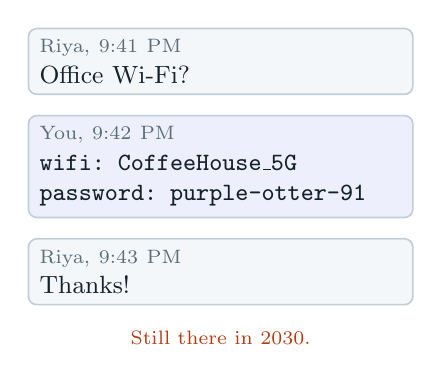
\begin{tikzpicture}[font=\small]
      \node[box, text width=4.6cm, align=left, fill=glass] (c1) {\muted{\scriptsize Riya, 9:41 PM}\\Office Wi-Fi?};
      \node[box, text width=4.6cm, align=left, fill=cobalt!8, below=0.25cm of c1] (c2)
        {\muted{\scriptsize You, 9:42 PM}\\\ttfamily wifi: CoffeeHouse\_5G\\password: purple-otter-91};
      \node[box, text width=4.6cm, align=left, fill=glass, below=0.25cm of c2] (c3) {\muted{\scriptsize Riya, 9:43 PM}\\Thanks!};
      \node[lbl, below=0.2cm of c3, text=ember] {Still there in 2030.};
    \end{tikzpicture}
  \end{columns}
\end{frame}
\note{[A] Think about the last time you sent someone a password. It's probably still sitting in that chat, in cloud backups, maybe in a screenshot. Messages last forever, but secrets shouldn't. And the websites that offer one-time links usually receive your secret in plain text, so you have to trust them completely.}

% ===================================================================================== 4
\begin{frame}{Objectives}
  \begin{enumerate}
    \item \hl{Self-destruct}: a note expires after \emph{N} views or \emph{T} time, whichever comes first.
    \item \hl{Zero knowledge}: the server stores only ciphertext and can never read a note.
    \item \hl{Correct under load}: two people can never both get the last view.
    \item \hl{Containerised}: the whole app runs from Docker images with one command.
    \item \hl{Deployed on a public cloud}: one Amazon EC2 instance, served over HTTPS.
  \end{enumerate}
\end{frame}
\note{[A] We set five objectives. Notes must self-destruct after a number of views or a time limit. The server must never be able to read them. The view limit must hold even when two people open the link at the same moment. The app must be fully containerised. And it must run on a public cloud, Amazon EC2, over HTTPS.}

% ===================================================================================== 5
\section{What Vanish does}
\begin{frame}{How it works for a user}
  \centering
  
\begin{tikzpicture}[node distance=0.55cm]
    \node[flowstep] (s1) {\textbf{Write}\\\scriptsize paste the secret, pick views and expiry};
    \node[flowstep, hot, right=of s1] (s2) {\textbf{Encrypt}\\\scriptsize AES-256-GCM, in the browser};
    \node[flowstep, right=of s2] (s3) {\textbf{Share}\\\scriptsize link with the key after \#, plus QR code};
    \node[flowstep, right=of s3] (s4) {\textbf{Open}\\\scriptsize one view used, decrypted on the device};
    \node[flowstep, right=of s4, draw=ember, text=ember] (s5) {\textbf{Gone}\\\scriptsize deleted at the last view or expiry};
    \foreach \a/\b in {s1/s2, s2/s3, s3/s4, s4/s5} \draw[arr] (\a) -- (\b);
  \end{tikzpicture}
  \vspace{1em}

  \begin{columns}[T]
    \column{0.3\textwidth}\centering \hl{1 to 10} views\\\muted{\small chosen by the sender}
    \column{0.3\textwidth}\centering \hl{5 min to 7 days}\\\muted{\small whichever limit comes first}
    \column{0.3\textwidth}\centering \hl{Optional passphrase}\\\muted{\small a second layer of encryption}
  \end{columns}
\end{frame}
\note{[B] Here's the flow. You write a secret and choose a view limit and an expiry. Your browser encrypts it with AES-256 before anything is sent. You get a link and a QR code. When the recipient opens it, one view is used and the note is decrypted on their device. At the last view, or when time runs out, it's gone for good. You can also add a passphrase as a second lock.}

% ===================================================================================== 6
\begin{frame}{Demo: creating a secret}
  \begin{columns}[T]
    \column{0.49\textwidth}\centering
    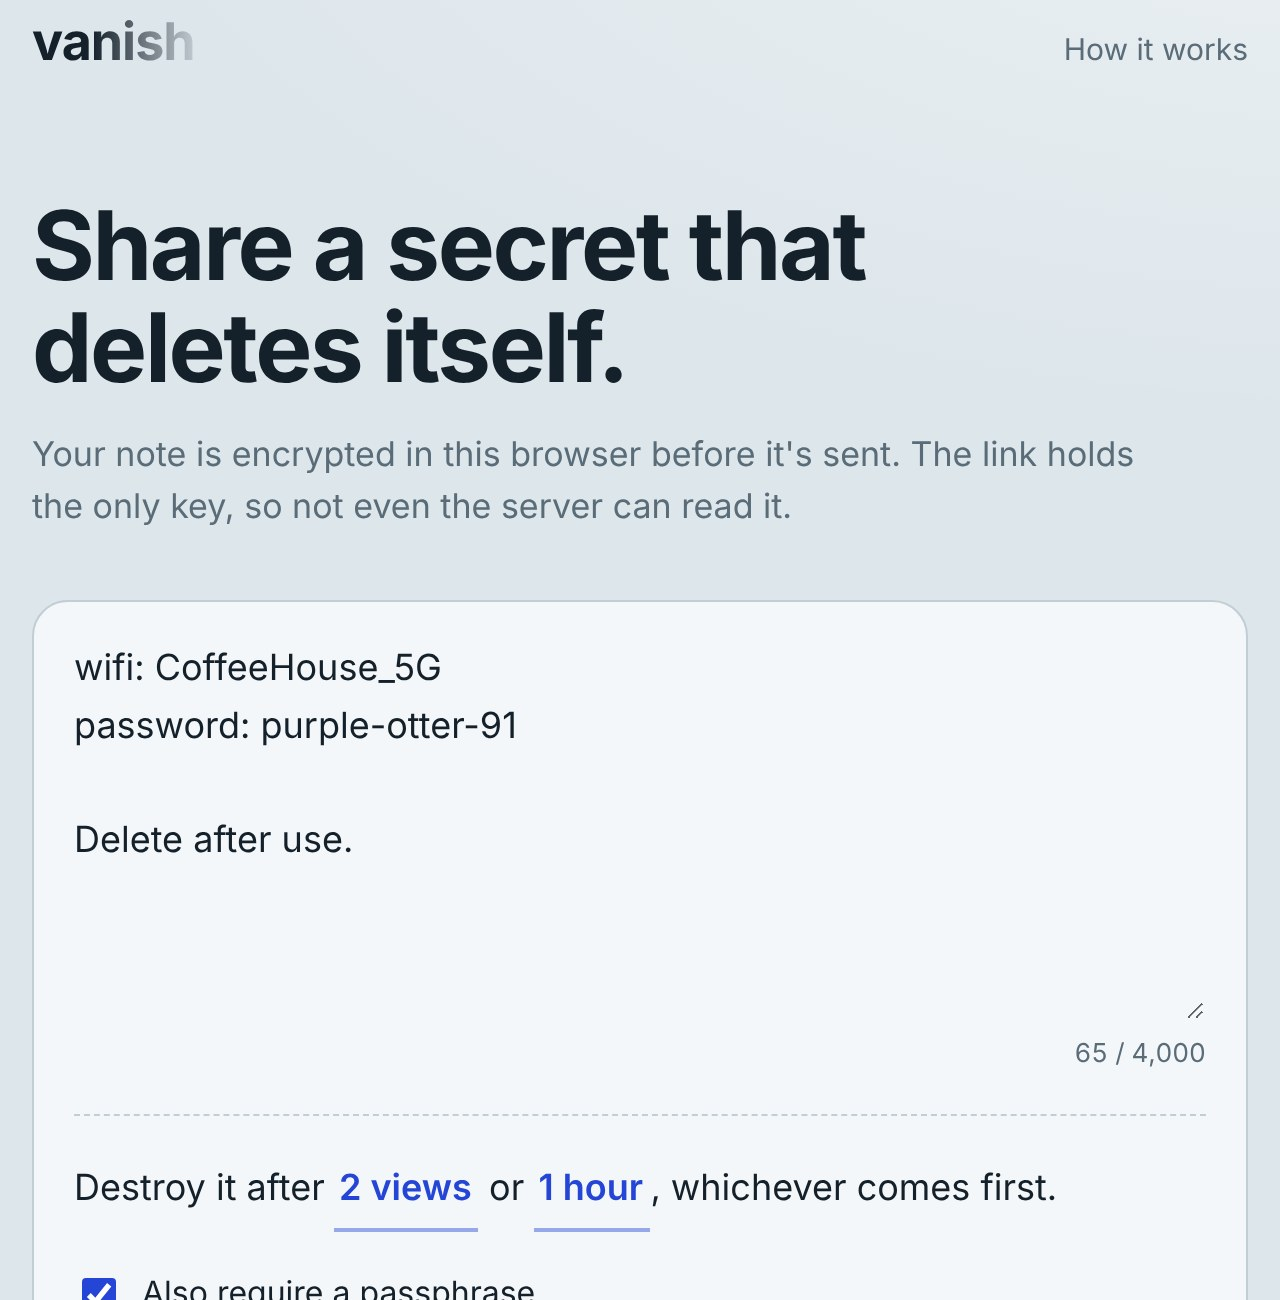
\includegraphics[width=0.84\linewidth]{img/create.jpg}\\[2pt]
    \muted{\scriptsize Write the note; 2 views or 1 hour; passphrase on}
    \column{0.49\textwidth}\centering
    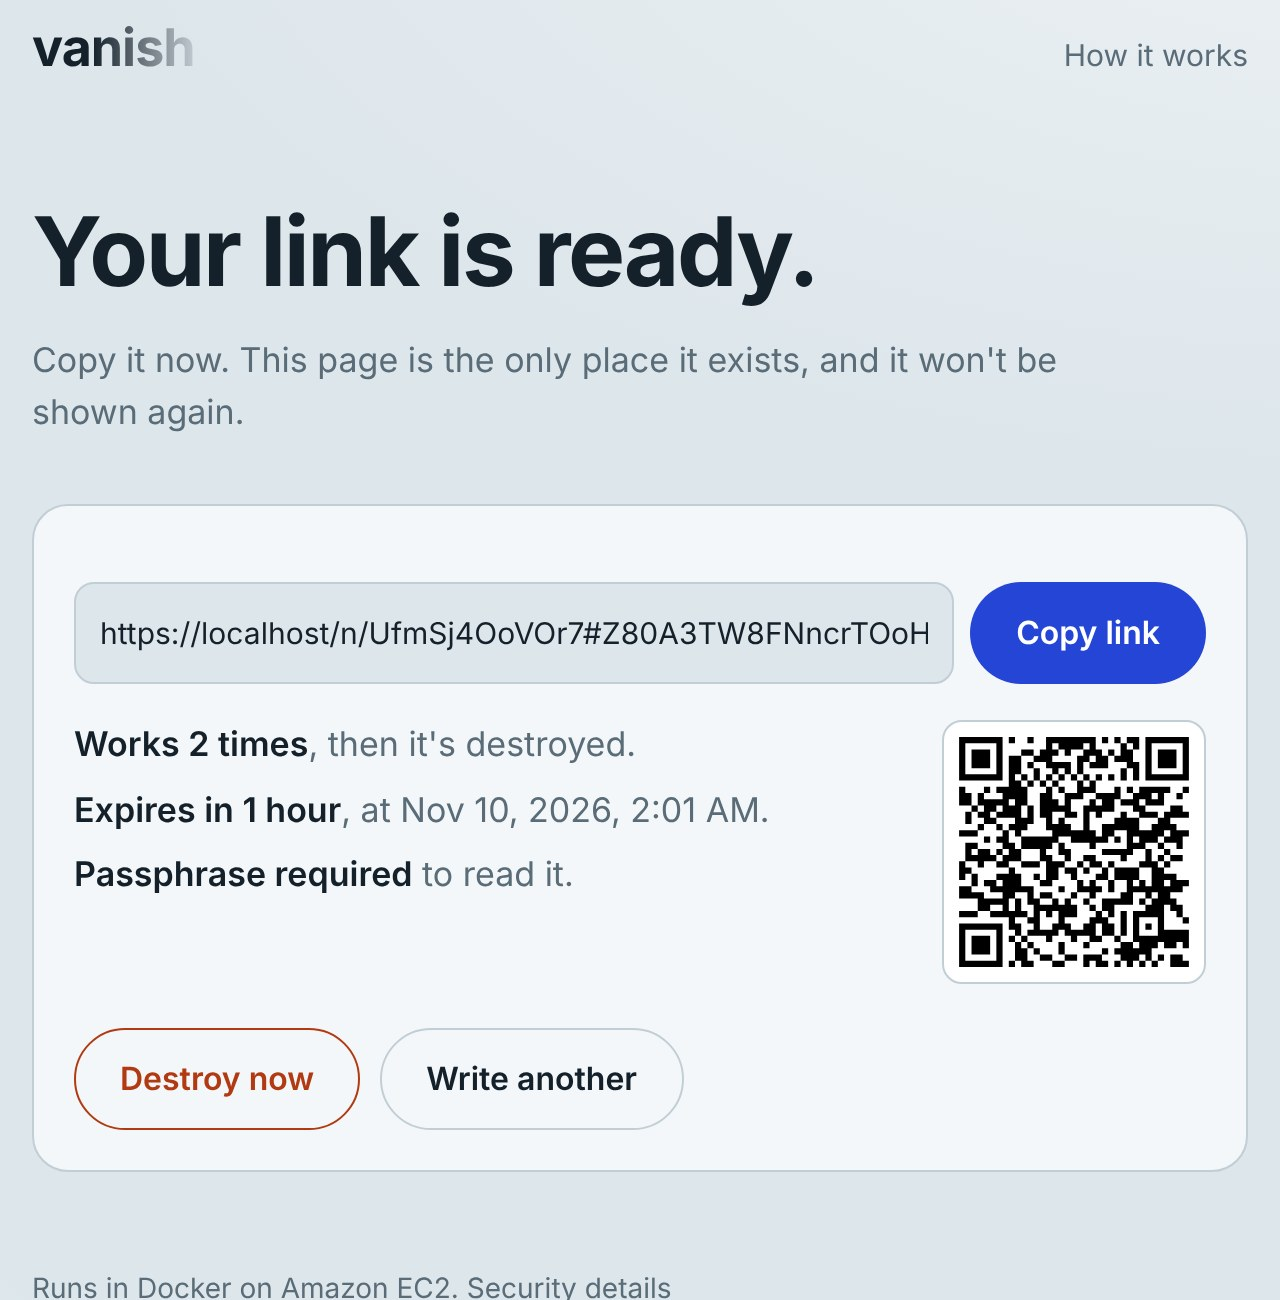
\includegraphics[width=0.84\linewidth]{img/link.jpg}\\[2pt]
    \muted{\scriptsize Encrypted in the browser; link and QR code returned}
  \end{columns}
\end{frame}
\note{[B] This is the app. I paste our café Wi-Fi password, choose two views or one hour, and add the passphrase ``mango''. When I press Create secret link, the text dissolves: it's being encrypted right here in the browser. On the right is the result: the link, a QR code for phones, and a summary of the rules. Only scrambled bytes were sent to the server.}

% ===================================================================================== 7
\begin{frame}{Demo: receiving it, then it vanishes}
  \begin{columns}[T]
    \column{0.32\textwidth}\centering
    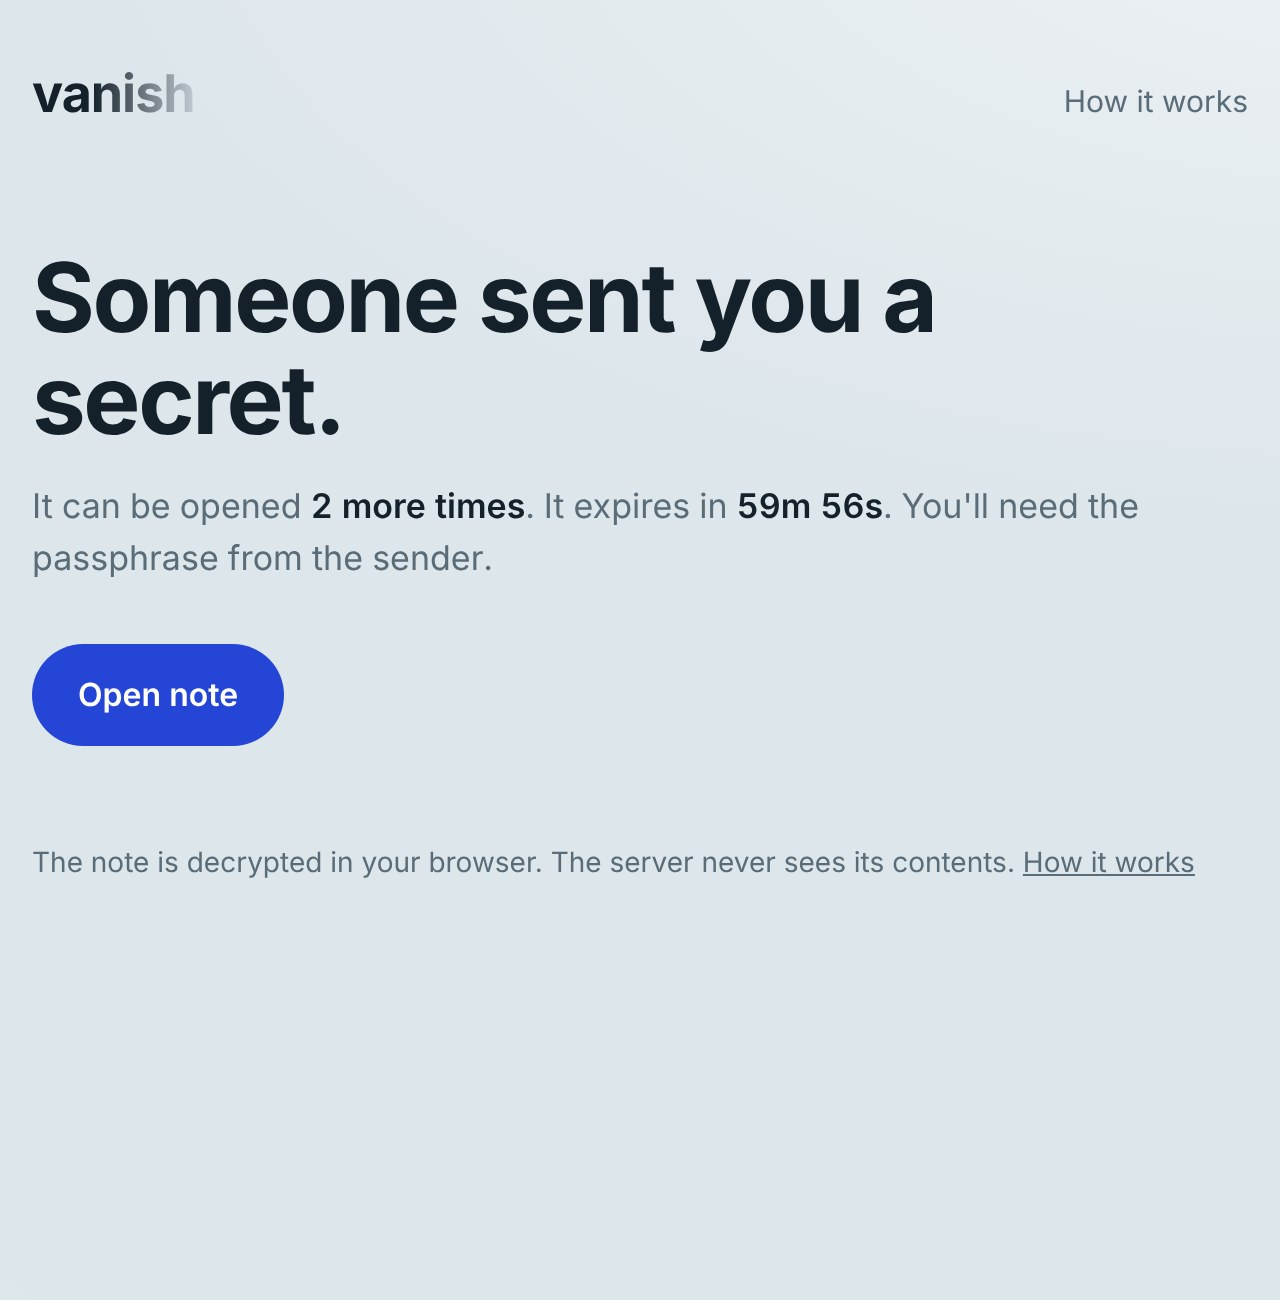
\includegraphics[width=\linewidth]{img/ready.jpg}\\[2pt]
    \muted{\scriptsize Countdown; opening the page uses no view}
    \column{0.32\textwidth}\centering
    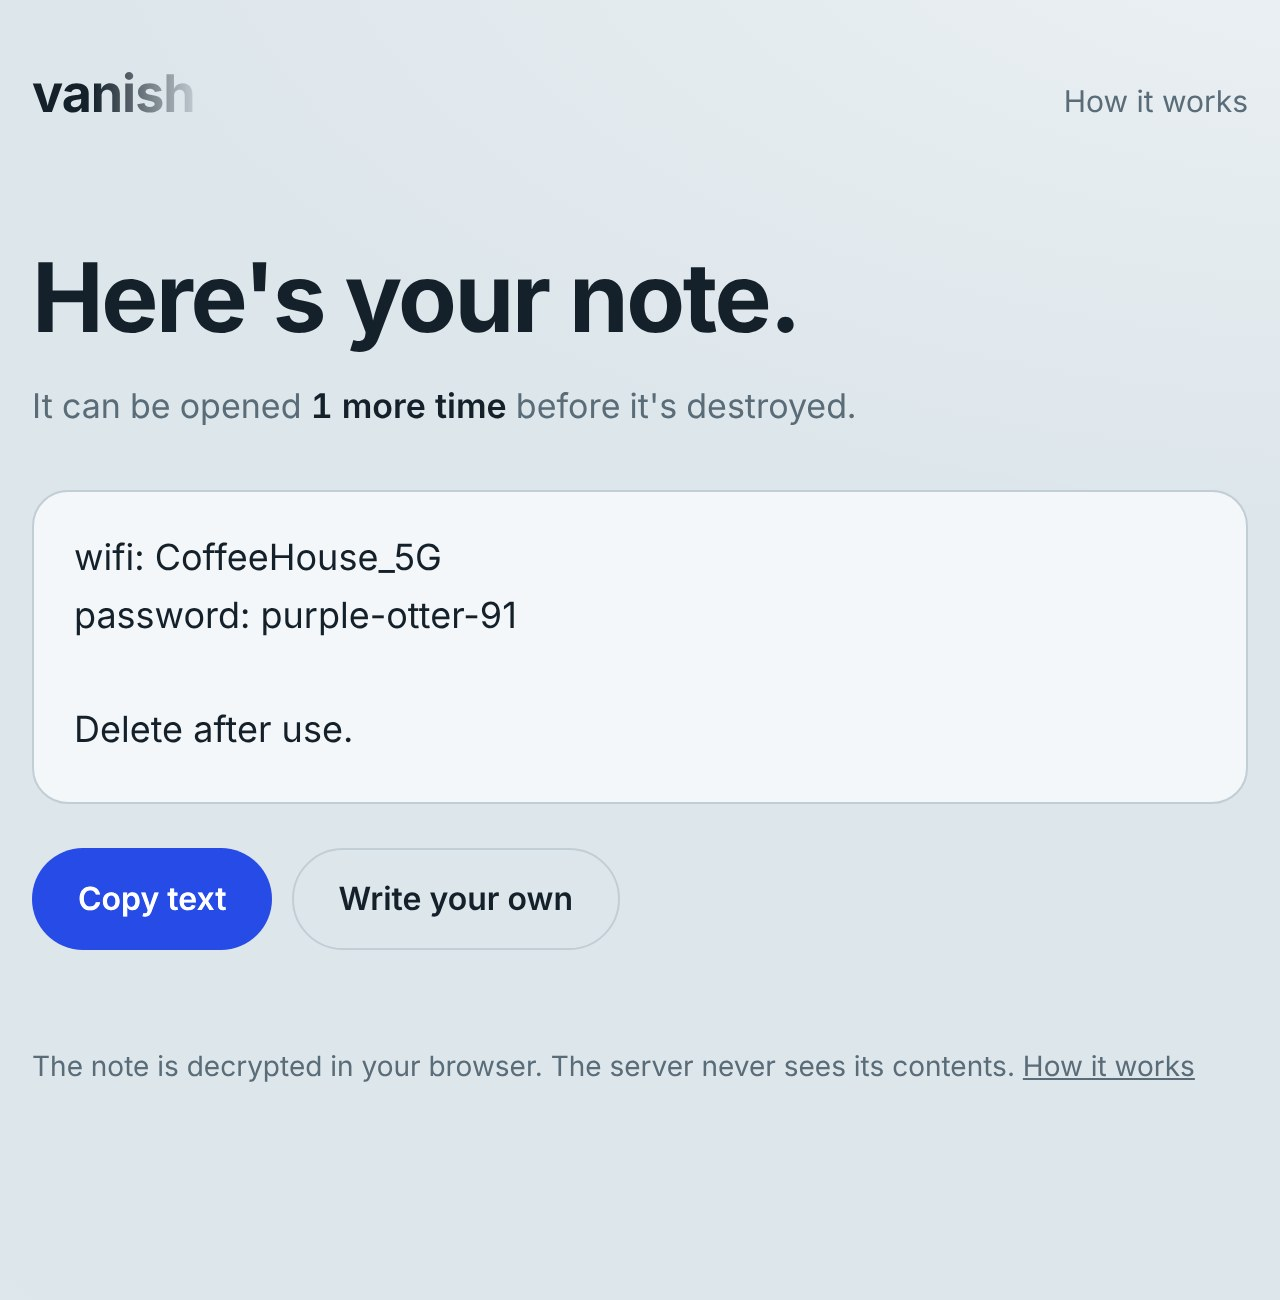
\includegraphics[width=\linewidth]{img/note.jpg}\\[2pt]
    \muted{\scriptsize Decrypted on the recipient's device}
    \column{0.32\textwidth}\centering
    
\includegraphics[width=\linewidth]{img/gone.jpg}\\[2pt]
    \muted{\scriptsize After the last view: nothing left}
  \end{columns}
\end{frame}
\note{[B] The recipient sees that a secret is waiting, how many views remain and a live countdown. Loading this page doesn't use a view, so chat apps that preview links can't burn it by accident. After entering the passphrase, the note is decrypted on their device. Once the last view is used, the server deletes it, and anyone opening the link again sees ``This note has vanished.''}

% ===================================================================================== 8
\section{Architecture}
\begin{frame}{Architecture on Amazon EC2}
  \centering
  \resizebox{\textwidth}{!}{%
  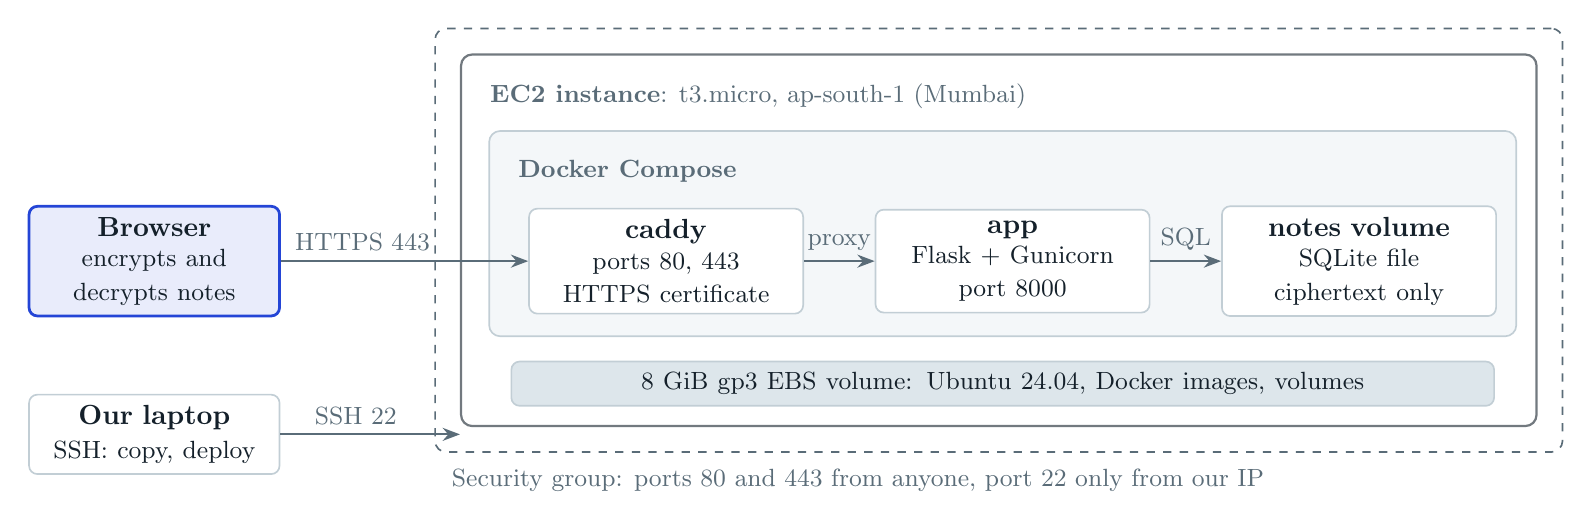
\begin{tikzpicture}[font=\normalsize, box/.append style={font=\normalsize}, hot/.append style={font=\normalsize}, lbl/.append style={font=\small}]
    \node[box, text width=3.2cm] (caddy) at (5.9,2.2) {\textbf{caddy}\\\small ports 80, 443\\HTTPS certificate};
    \node[box, text width=3.2cm] (app) at (10.3,2.2) {\textbf{app}\\\small Flask + Gunicorn\\port 8000};
    \node[box, text width=3.2cm] (vol) at (14.7,2.2) {\textbf{notes volume}\\\small SQLite file\\ciphertext only};
    \node[lbl, anchor=south west] (dcl) at ($(caddy.north west)+(-0.25,0.2)$) {\textbf{Docker Compose}};
    \begin{scope}[on background layer]
      \node[group, fill=glass, fit=(caddy)(app)(vol)(dcl)] (compose) {};
    \end{scope}
    \node[box, fill=fog, text width=12.2cm, anchor=north] (ebs) at ($(compose.south)+(0,-0.3)$)
      {\small 8 GiB gp3 EBS volume: Ubuntu 24.04, Docker images, volumes};
    \node[lbl, anchor=south west] (ecl) at ($(compose.north west)+(-0.1,0.15)$) {\textbf{EC2 instance}: t3.micro, ap-south-1 (Mumbai)};
    \begin{scope}[on background layer]
      \node[group, line width=0.8pt, draw=ink!60, fit=(compose)(ebs)(ecl)] (ec2) {};
      \node[group, dashed, draw=mist, inner sep=9pt, fit=(ec2)] (sg) {};
    \end{scope}
    \node[lbl, anchor=north west] at ($(sg.south west)+(0.1,-0.08)$) {Security group: ports 80 and 443 from anyone, port 22 only from our IP};
    \node[hot, text width=2.9cm] (browser) at (-0.6,2.2) {\textbf{Browser}\\\small encrypts and\\decrypts notes};
    \node[box, text width=2.9cm] (laptop) at (-0.6,0.0) {\textbf{Our laptop}\\\small SSH: copy, deploy};
    \draw[arr] (browser) -- node[lbl, above, pos=0.33] {HTTPS 443} (caddy);
    \draw[arr] (caddy) -- node[lbl, above] {proxy} (app);
    \draw[arr] (app) -- node[lbl, above] {SQL} (vol);
    \draw[arr] (laptop) -- node[lbl, above, pos=0.42] {SSH 22} (laptop -| ec2.west);
  \end{tikzpicture}}
\end{frame}
\note{[C] Everything runs on one Amazon EC2 virtual machine: a t3.micro running Ubuntu in the Mumbai region. A security group, AWS's firewall, lets anyone in on ports 80 and 443, but SSH only from our own IP. Inside, Docker Compose runs two containers. Caddy is the public web server: it gets a free HTTPS certificate and forwards requests to our app container, Flask with Gunicorn. The app keeps notes in a SQLite file on a Docker volume, which lives on the instance's EBS disk.}

% ===================================================================================== 9
\begin{frame}{Cloud services and features used}
  \small
  \begin{tabularx}{\textwidth}{@{}l X l@{}}
    \toprule
    \textbf{Service / feature} & \textbf{How Vanish uses it} & \textbf{Setting} \\
    \midrule
    EC2 instance        & Runs Docker and both containers                    & t3.micro, 2 vCPU, 1 GiB \\
    AMI                 & Operating system image                              & Ubuntu Server 24.04 LTS \\
    User data           & Installs Docker and swap on first boot              & \code{deploy/user-data.sh} \\
    Instance metadata   & \code{deploy.sh} looks up the public IP (IMDSv2)     & 169.254.169.254 \\
    Security group      & Stateful firewall in front of the instance          & 22 (our IP), 80, 443 \\
    Key pair            & Password-less SSH login                              & RSA, \code{.pem} \\
    EBS volume          & Disk for OS, images and the notes database          & 8 GiB gp3 \\
    Public IPv4         & Address users connect to; HTTPS certificate is for it & auto-assigned \\
    EC2 monitoring      & CPU, network and status checks                      & Monitoring tab \\
    \bottomrule
  \end{tabularx}
\end{frame}
\note{[C] These are the EC2 features we used. The instance type and the Ubuntu AMI. A user-data script that installs Docker automatically at first boot. The instance metadata service, which our deploy script queries for the public IP. A security group as the firewall, a key pair for SSH, an 8 GiB EBS volume for storage, the public IPv4 address, and EC2's built-in monitoring.}

% ===================================================================================== 10
\section{Implementation}
\begin{frame}{Zero-knowledge encryption: the key never reaches the server}
  \centering
  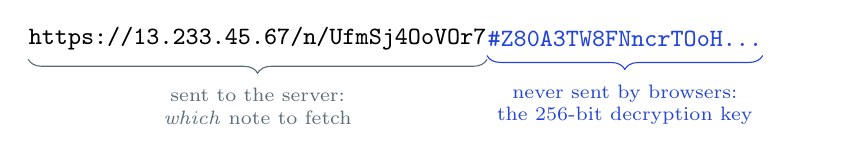
\begin{tikzpicture}
    \node[font=\ttfamily\small, inner sep=0] (a) {https://13.233.45.67/n/UfmSj4OoVOr7};
    \node[font=\ttfamily\small, inner sep=0, anchor=west, text=cobalt] (b) at (a.east) {\#Z80A3TW8FNncrTOoH\dots};
    \draw[decorate, decoration={brace, mirror, amplitude=5pt}, draw=mist] ([yshift=-3pt]a.south west) -- ([yshift=-3pt]a.south east)
      node[midway, below=7pt, lbl, text width=5.2cm, align=center] {sent to the server:\\\textit{which} note to fetch};
    \draw[decorate, decoration={brace, mirror, amplitude=5pt}, draw=cobalt] ([yshift=-3pt]b.south west) -- ([yshift=-3pt]b.south east)
      node[midway, below=7pt, font=\scriptsize, text=cobalt, text width=4.6cm, align=center] {never sent by browsers:\\the 256-bit decryption key};
  \end{tikzpicture}
  \vspace{0.8em}

  \begin{columns}[T]
    \column{0.48\textwidth}
    \begin{itemize}\small
      \item Browser generates a random 256-bit key and encrypts with \hl{AES-256-GCM} (Web Crypto API).
      \item Only \code{\{ciphertext, iv\}} is uploaded.
    \end{itemize}
    \column{0.48\textwidth}
    \begin{itemize}\small
      \item Optional passphrase: second layer, key from \hl{PBKDF2-SHA256}, 310,000 rounds.
      \item GCM is authenticated: tampered data fails to decrypt.
    \end{itemize}
  \end{columns}
\end{frame}
\note{[B] This is the core idea. The part of the link before the hash tells the server which note to fetch. The part after the hash is the 256-bit decryption key, and browsers never send that part to any server. So our EC2 instance only ever stores scrambled ciphertext. Encryption uses AES-256-GCM from the browser's built-in Web Crypto API, and the optional passphrase adds a second layer derived with PBKDF2.}

% ===================================================================================== 11
\begin{frame}{The API: five small endpoints}
  \small
  \begin{tabularx}{\textwidth}{@{}l l X@{}}
    \toprule
    \textbf{Method} & \textbf{Path} & \textbf{What it does} \\
    \midrule
    \code{POST}   & \code{/api/notes}             & Store \code{ciphertext}, \code{iv}, view limit (1--10), expiry (5 min--7 days) \\
    \code{GET}    & \code{/api/notes/\{id\}}      & Views left and expiry; \hl{does not use a view} (safe for link previews) \\
    \code{POST}   & \code{/api/notes/\{id\}/open} & Atomically use one view and return the ciphertext; \code{410 Gone} afterwards \\
    \code{DELETE} & \code{/api/notes/\{id\}}      & Destroy early with the secret delete token (stored as a SHA-256 hash) \\
    \code{GET}    & \code{/api/health}            & Liveness check used by the Docker health check \\
    \bottomrule
  \end{tabularx}
  \vspace{0.8em}

  \muted{A background thread deletes expired notes every 60 seconds; every read also checks the expiry time.}
\end{frame}
\note{[A] The backend is one Python file with five endpoints. Creating a note stores only ciphertext. Reading the metadata never uses a view, which is why WhatsApp previews can't burn a note. Opening uses one view atomically. There's an early-destroy endpoint protected by a secret token, and a health check that Docker uses. A background thread deletes expired notes every minute.}

% ===================================================================================== 12
\begin{frame}[fragile]{Atomic view counting: exactly one winner}
  \begin{columns}[T]
    \column{0.56\textwidth}
\begin{lstlisting}[language=SQL]
UPDATE notes
   SET view_count = view_count + 1
 WHERE id = ?
   AND view_count < max_views
   AND expires_at > ?
RETURNING ciphertext, iv, max_views,
          view_count, expires_at;
\end{lstlisting}
    \small\muted{From \code{open\_note} in \code{app/main.py}. If no row comes back, the API answers \code{410 Gone}.}
    \column{0.40\textwidth}
    \begin{block}{Why one statement?}
      \small
      Check and update happen together, so two people opening the \emph{last} view at the same moment can't both succeed.
    \end{block}
    \vspace{0.4em}
    \begin{exampleblock}{Tested}
      \small 8 simultaneous requests on a 1-view note: \textbf{1} gets the note, \textbf{7} get \code{410}.
    \end{exampleblock}
  \end{columns}
\end{frame}
\note{[A] The most important line of backend code is this single SQL statement. It increases the view count only if the note still has views left and hasn't expired, and returns the note in the same step. Because the check and the update are one atomic operation, two people can't both get the last view. Our test fires eight requests at the same moment at a one-view note: exactly one wins and seven get 410 Gone.}

% ===================================================================================== 13
\section{Docker and deployment}
\begin{frame}[fragile]{Containerising the app: the Dockerfile}
  \begin{columns}[T]
    \column{0.56\textwidth}
\begin{lstlisting}[language=Docker]
FROM python:3.13-slim
ENV DB_PATH=/data/vanish.db
WORKDIR /app
COPY requirements.txt .
RUN pip install --no-cache-dir \
        -r requirements.txt
COPY app/ .
RUN useradd --system --uid 10001 vanish \
 && mkdir -p /data \
 && chown vanish:vanish /data
USER vanish
EXPOSE 8000
HEALTHCHECK CMD python -c "..."  # GET /api/health
CMD ["gunicorn", "--bind", "0.0.0.0:8000",
     "--workers", "1", "--threads", "8",
     "main:app"]
\end{lstlisting}
    \column{0.40\textwidth}
    \begin{itemize}\small
      \item \hl{Slim base image}: small download, fewer packages to patch.
      \item \hl{Dependencies first}: code changes don't re-run \code{pip}.
      \item \hl{Non-root user}: a compromised app can't take over the container.
      \item \hl{Health check}: Docker flags the container if the API stops answering.
      \item \hl{Gunicorn}: production web server, 8 threads.
    \end{itemize}
  \end{columns}
\end{frame}
\note{[C] This is our Dockerfile. It starts from the official slim Python image, installs Flask and Gunicorn first so that code changes rebuild quickly, copies the app, and runs it as a non-root user. A health check calls our API every 30 seconds, and Gunicorn serves the app with eight threads.}

% ===================================================================================== 14
\begin{frame}[fragile]{Two containers: Docker Compose and Caddy}
  \begin{columns}[T]
    \column{0.55\textwidth}
    \small\textbf{compose.yaml} \muted{(abridged)}
\begin{lstlisting}[language=yaml]
services:
  app:
    image: vanish-app:1.0
    build: .
    volumes: ["notes:/data"]
    ports: ["127.0.0.1:8000:8000"]   # private
  caddy:
    image: caddy:2.11
    ports: ["80:80", "443:443"]       # public
    environment:
      SITE_ADDRESS: ${SITE_ADDRESS}
    volumes:
      - ./Caddyfile:/etc/caddy/Caddyfile:ro
      - caddy_data:/data
\end{lstlisting}
    \column{0.41\textwidth}
    \small\textbf{Caddyfile}
\begin{lstlisting}
{
  default_sni {$SITE_ADDRESS}
}
{$SITE_ADDRESS} {
  tls {
    issuer acme {
      profile shortlived
    }
  }
  encode zstd gzip
  reverse_proxy app:8000
}
\end{lstlisting}
    \small\muted{Free Let's Encrypt certificate for the public IP, renewed automatically.}
  \end{columns}
\end{frame}
\note{[C] Docker Compose runs two containers. The app's port is bound to localhost only, so the internet can reach it only through Caddy. Notes live in a named volume, so they survive restarts and rebuilds. On the right is the entire Caddyfile: it requests a free Let's Encrypt certificate for our IP address and forwards every request to the app. HTTPS isn't optional here: browsers only allow the Web Crypto API on secure pages.}

% ===================================================================================== 15
\begin{frame}{Build once, ship the image to EC2}
  \centering
  \resizebox{\textwidth}{!}{%
  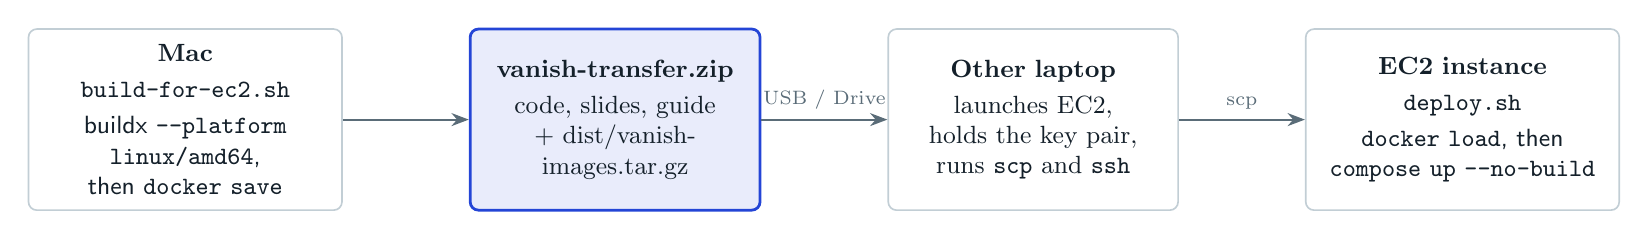
\begin{tikzpicture}[node distance=1.6cm, every node/.append style={font=\normalsize}]
    \node[box, text width=3.7cm, minimum height=2.3cm] (mac) {\textbf{Mac}\\[2pt]\small\ttfamily build-for-ec2.sh\\[2pt]\rmfamily\sffamily buildx \texttt{-{}-platform linux/amd64}, then \texttt{docker save}};
    \node[hot, text width=3.4cm, minimum height=2.3cm, right=of mac] (zip) {\textbf{vanish-transfer.zip}\\[2pt]\small code, slides, guide\\+ dist/vanish-images.tar.gz};
    \node[box, text width=3.4cm, minimum height=2.3cm, right=of zip] (pc) {\textbf{Other laptop}\\[2pt]\small launches EC2, holds the key pair, runs \texttt{scp} and \texttt{ssh}};
    \node[box, text width=3.7cm, minimum height=2.3cm, right=of pc] (ec2) {\textbf{EC2 instance}\\[2pt]\small\ttfamily deploy.sh\\[2pt]\rmfamily\sffamily \texttt{docker load}, then \texttt{compose up -{}-no-build}};
    \draw[arr] (mac) -- (zip);
    \draw[arr] (zip) -- node[lbl, above] {USB / Drive} (pc);
    \draw[arr] (pc) -- node[lbl, above] {scp} (ec2);
  \end{tikzpicture}}
  \vspace{0.9em}

  \begin{alertblock}{Why \texttt{linux/amd64}?}
    \small Apple Silicon Macs build \texttt{arm64} images by default, but a t3.micro has an Intel/AMD processor. A wrong image fails with \emph{exec format error}, so \code{deploy.sh} checks the architecture before starting.
  \end{alertblock}
\end{frame}
\note{[C] We build the images once and ship them. On the Mac, one script builds the app image for linux/amd64, downloads Caddy, and saves both into a single archive inside the project zip. We carry that zip to the laptop we deploy from, copy it to EC2 with scp, and our deploy script loads the images and starts them, with no build on the server. The platform flag matters: Apple Silicon builds arm64 by default, which won't run on a t3.micro, so the deploy script checks this before starting.}

% ===================================================================================== 16
\begin{frame}[fragile]{Deploying on EC2 in four steps}
  \begin{columns}[T]
    \column{0.46\textwidth}
    \begin{enumerate}\small
      \item \textbf{Launch} a t3.micro with Ubuntu 24.04, key pair \code{vanish-key}, HTTP + HTTPS open, SSH from our IP, and \code{user-data.sh} pasted in.
      \item \textbf{Copy} the zip with \code{scp}.
      \item \textbf{Unzip} and run \code{deploy.sh}.
      \item \textbf{Open} \code{https://<public-ip>}.
    \end{enumerate}
    \column{0.52\textwidth}
\begin{lstlisting}[language=bash]
# from the laptop
scp -i vanish-key.pem vanish-transfer.zip \
    ubuntu@13.233.45.67:~
ssh -i vanish-key.pem ubuntu@13.233.45.67

# on the instance
unzip vanish-transfer.zip && cd vanish
bash deploy/deploy.sh
docker compose ps
docker compose logs caddy   # certificate
\end{lstlisting}
  \end{columns}
  \vspace{0.3em}
  \muted{\small \code{deploy.sh} asks the instance metadata service for the public IP, writes it to \code{.env}, loads the images and starts both containers.}
\end{frame}
\note{[C] Deployment takes four steps. We launch a t3.micro with Ubuntu, open HTTP and HTTPS, restrict SSH to our IP, and paste our user-data script, which installs Docker at first boot. Then we copy the zip over with scp, log in with ssh, unzip it and run one script. It finds the public IP from the instance metadata service, loads the images, starts both containers, and Caddy obtains the certificate within a minute.}

% ===================================================================================== 17
\section{Results}
\begin{frame}{Security measures}
  \begin{columns}[T]
    \column{0.48\textwidth}
    \textbf{Data}
    \begin{itemize}\small
      \item Server stores ciphertext, timestamps and counters only
      \item Key in the URL fragment; removed from the address bar after opening
      \item Delete tokens stored as SHA-256 hashes
      \item Notes up to 4,000 characters; 20 new notes per minute per IP
    \end{itemize}
    \column{0.48\textwidth}
    \textbf{Infrastructure}
    \begin{itemize}\small
      \item Security group: only ports 22 (our IP), 80 and 443
      \item App port bound to localhost; only Caddy is public
      \item Container runs as a non-root user
      \item HTTPS everywhere, HSTS, strict Content-Security-Policy, no referrer
    \end{itemize}
  \end{columns}
\end{frame}
\note{[B] Security works in two layers. For data: the server only ever sees ciphertext, the key lives in the URL fragment and is removed from the address bar after opening, delete tokens are hashed, and note creation is rate-limited. For infrastructure: the security group exposes only three ports, the app container isn't directly reachable, it runs as a non-root user, and every response is served over HTTPS with strict browser security headers.}

% ===================================================================================== 18
\begin{frame}{Testing}
  \begin{columns}[T]
    \column{0.40\textwidth}
    \begin{block}{Automated tests (pytest)}
      \centering\vspace{2pt}
      {\Huge\bfseries\color{okgreen} 16 / 16}\\[2pt]
      \small passing
    \end{block}
    \small
    \begin{itemize}
      \item View counting and burn-on-last-view
      \item 8 concurrent opens: exactly 1 winner
      \item Expiry and cleanup, delete tokens
      \item Input validation, rate limit, pages
    \end{itemize}
    \column{0.56\textwidth}
    \textbf{Live checks on the EC2 deployment}
    \small
    \begin{enumerate}
      \item HTTPS loads; \code{http://} redirects to \code{https://}
      \item Create a 2-view note; open it twice; third open shows ``vanished''
      \item Wrong passphrase rejected; right one decrypts
      \item \emph{Destroy now} works; missing key detected
      \item Port 8000 unreachable from the internet
      \item Notes survive \code{docker compose restart}
      \item Database holds ciphertext only
    \end{enumerate}
  \end{columns}
\end{frame}
\note{[A] We tested at two levels. Sixteen automated tests run against the real Flask app and all pass, including the concurrency test. Then on the live EC2 instance we checked HTTPS and the redirect, the full view and burn cycle, the passphrase, early destroy, that port 8000 is closed to the internet, that notes survive a restart, and that the database only contains ciphertext.}

% ===================================================================================== 19
\begin{frame}{Cost}
  \begin{columns}[c]
    \column{0.58\textwidth}
    \small
    \begin{tabularx}{\linewidth}{@{}X r@{}}
      \toprule
      \textbf{Item (ap-south-1, 24/7)} & \textbf{USD / month} \\
      \midrule
      t3.micro instance (\$0.0112 / hour) & $\approx$ 8.20 \\
      Public IPv4 address               & $\approx$ 3.65 \\
      8 GiB gp3 EBS volume              & $\approx$ 0.75 \\
      \midrule
      \textbf{Total}                    & $\approx$ \textbf{12.60} \\
      \bottomrule
    \end{tabularx}
    \column{0.38\textwidth}
    \begin{exampleblock}{Paid by the Free plan}
      \small New AWS accounts get \textbf{\$100 credit}; t3.micro is Free Tier eligible. Our out-of-pocket cost: \textbf{INR 0}.
    \end{exampleblock}
    \vspace{0.3em}
    \muted{\small Stopping the instance when idle leaves only the disk charge.}
  \end{columns}
\end{frame}
\note{[C] Running all month, the instance, its public IP and its disk cost about twelve and a half dollars. New AWS accounts on the Free plan get a hundred dollars of credit and t3.micro is Free Tier eligible, so our out-of-pocket cost was zero. When we aren't using it, we stop the instance, and only the small disk charge remains.}

% ===================================================================================== 20
\section{Conclusion}
\begin{frame}{Challenges and lessons learned}
  \begin{itemize}
    \item \hl{CPU architecture matters.} Images built on an Apple Silicon Mac are \code{arm64}; EC2 t3 is \code{amd64}. Fixed with \code{buildx -{}-platform linux/amd64} and a check in \code{deploy.sh}.
    \item \hl{Browser crypto needs HTTPS.} Web Crypto is disabled on plain \code{http://}, so Caddy with a Let's Encrypt IP certificate is part of the design.
    \item \hl{Public IPs change.} Stopping and starting the instance gives a new IP; re-running \code{deploy.sh} picks it up automatically.
    \item \hl{1 GiB of RAM is tight.} User data adds 1 GiB of swap so builds on the instance never run out of memory.
  \end{itemize}
\end{frame}
\note{[B] We learned a few things the hard way. CPU architecture matters: images from an Apple Silicon Mac won't run on an Intel EC2 instance unless you build for linux/amd64. Browser encryption requires HTTPS, so getting a certificate without a domain became part of the design. Public IPs change when you stop an instance, so the deploy script re-detects it. And a one-gigabyte instance needs swap to build images safely.}

% ===================================================================================== 21
\begin{frame}{Limitations and future work}
  \begin{columns}[T]
    \column{0.47\textwidth}
    \textbf{Limitations}
    \begin{itemize}\small
      \item Anyone holding the full link can read the note; use a passphrase for sensitive data
      \item One instance: no redundancy if it stops
      \item SQLite on one disk: fine for this scale, not for many servers
    \end{itemize}
    \column{0.49\textwidth}
    \textbf{Future work}
    \begin{itemize}\small
      \item Custom domain and an Elastic IP for a stable address
      \item Managed database (Amazon RDS) and two instances behind a load balancer
      \item Image registry (Amazon ECR) and a CI pipeline for builds
      \item File attachments, encrypted the same way
    \end{itemize}
  \end{columns}
\end{frame}
\note{[B] Some honest limits. Anyone with the full link can read the note, so sensitive notes should use a passphrase. One instance means no redundancy, and SQLite suits a single server. Next steps would be a custom domain with a stable Elastic IP, a managed database with two instances behind a load balancer, a container registry with automated builds, and encrypted file attachments.}

% ===================================================================================== 22
\begin{frame}{Summary}
  \begin{columns}[c]
    \column{0.62\textwidth}
    \begin{itemize}
      \item Secrets that \hl{self-destruct} after N views or T time
      \item \hl{Zero-knowledge}: encrypted in the browser, ciphertext on the server
      \item \hl{Atomic} view counting, verified under concurrency
      \item Packaged as \hl{Docker images}, run with Docker Compose
      \item Deployed on \hl{Amazon EC2} over HTTPS, for INR 0
    \end{itemize}
    \column{0.34\textwidth}
    \centering
    {\Large\bfseries Thank you}\\[6pt]
    \muted{Questions?}\\[14pt]
    \small \memberA\\\memberB\\\memberC
  \end{columns}
\end{frame}
\note{[B] To sum up: Vanish lets you share a secret that destroys itself, it never sees your data in plain text, its view limits hold under concurrent access, and the whole thing is packaged with Docker and running on Amazon EC2 over HTTPS, at no cost to us. Thank you for watching.}

\end{document}
